%%%%%%%%%%%%%%%%%%%%%%% file template.tex %%%%%%%%%%%%%%%%%%%%%%%%%
%
% This is a general template file for the LaTeX package SVJour3
% for Springer journals.          Springer Heidelberg 2010/09/16
%
% Copy it to a new file with a new name and use it as the basis
% for your article. Delete % signs as needed.
%
% This template includes a few options for different layouts and
% content for various journals. Please consult a previous issue of
% your journal as needed.
%
%%%%%%%%%%%%%%%%%%%%%%%%%%%%%%%%%%%%%%%%%%%%%%%%%%%%%%%%%%%%%%%%%%%

%\documentclass{svjour3}                     % onecolumn (standard format)
\documentclass[smallcondensed, natbib]{svjour3}     % onecolumn (ditto)
%\documentclass[smallextended,natbib]{svjour3}       % onecolumn (second format)
%\documentclass[twocolumn]{svjour3}          % twocolumn
%
\smartqed  % flush right qed marks, e.g. at end of proof
%
\usepackage{graphicx}
\usepackage{geometry}
\geometry{
  a4paper,         % or letterpaper
  textwidth=16cm,  % llncs has 12.2cm
  textheight=22cm, % llncs has 19.3cm
  heightrounded,   % integer number of lines
  hratio=1:1,      % horizontally centered
  vratio=2:3,      % not vertically centered
}
\usepackage{mathptmx}      % use Times fonts if available on your TeX system
%
% insert here the call for the packages your document requires
%\usepackage{latexsym}
% etc.
%
% please place your own definitions here and don't use \def but
% \newcommand{}{}
%
% Insert the name of "your journal" with
\journalname{Memetic Computing}
%

%% The amssymb package provides various useful mathematical symbols
\usepackage{amssymb}
%% The amsthm package provides extended theorem environments
%% \usepackage{amsthm}

%% The lineno packages adds line numbers. Start line numbering with
%% \begin{linenumbers}, end it with \end{linenumbers}. Or switch it on
%% for the whole article with \linenumbers.
%% \usepackage{lineno}
\usepackage{lineno,hyperref}
\hypersetup{breaklinks=true}
\modulolinenumbers[5]
\setcitestyle{square, sort,comma,numbers}
\setcitestyle{citesep={,}}
%\journal{Journal of Computer and System Sciences}


%%%%%%======================== Our custom packages =====================

%GN/SD added BEGIN-->
	\usepackage{color}						% http://latexcolor.com/
	
	\definecolor{gn_green}{rgb}{0.0, 0.5, 0.0}
	\def \TN#1{\textcolor{gn_green}{~#1}}			% Thieu Nguyen
	
	\def \BM#1{\textcolor{blue}{~#1}}				% Binh Minh Nguyen
	
	\definecolor{tn_orange}{rgb}{1.0, 0.49, 0.0}		
	\def \GN#1{\textcolor{tn_orange}{~#1}}			% Giang Nguyen
	
	\definecolor{at_bleudefrance}{rgb}{0.19, 0.55, 0.91}		
	\def \AT#1{\textcolor{at_bleudefrance}{~#1}}		% Tu Nguyen
	
	\usepackage{rotating}
	\usepackage{booktabs}
	\usepackage{adjustbox}
	
	\makeatletter
		\newcommand\primitiveinput[1]
		{\@@input #1 }
	\makeatother
	
	\newcommand{\multilinecol}[1]{%
		\begin{tabular}{@{}c@{}}#1\end{tabular}%
	}
%<-- GN/SD added END


%% ====== Table =====
\usepackage{multirow, array}

%% ====== Algorithms ======
\usepackage{algorithm}
\usepackage[noend]{algpseudocode}
\usepackage{amsmath}
\usepackage{tabu}
\usepackage[dvipsnames]{xcolor}

\usepackage{array}
\newcolumntype{L}[1]{>{\raggedright\let\newline\\\arraybackslash\hspace{2pt}}m{#1}}
\newcolumntype{C}[1]{>{\centering\let\newline\\\arraybackslash\hspace{2pt}}m{#1}}
\newcolumntype{R}[1]{>{\raggedleft\let\newline\\\arraybackslash\hspace{2pt}}m{#1}}

\algnewcommand\algorithmicforeach{\textbf{for each}}
\algdef{S}[FOR]{ForEach}[1]{\algorithmicforeach\ #1\ \algorithmicdo}
\newcommand{\Break}{\State \textbf{break} }

\renewcommand{\familydefault}{\rmdefault}
\renewcommand{\thetable}{\arabic{table}}


%%%%%%======================== End our custom packages =====================

\begin{document}

%\begin{frontmatter}
%%%==== Title Page ====%%%

\title{Efficient Time-series Forecasting using Neural Network and Opposition-based Coral Reefs Optimization}
%\title{An Effective Workload Prediction Model for Distributed Applications using Multi-Layer Neural Network and Opposition-based Coral Reefs Optimization}
%\title{A Comparative Study of Multi-Layer Neural Network and Opposition-based Coral Reefs Optimization Modeling in Time Series Prediction}
%\tnotetext[mytitlenote]{Fully documented templates are available in the elsarticle package on \href{http://www.ctan.org/tex-archive/macros/latex/contrib/elsarticle}{CTAN}.}


%\author{Thieu Nguyen\inst{1} \and Tu Nguyen\inst{1}\and 
%Binh Minh Nguyen\inst{1}\thanks{Corresponding author.}\and Giang Nguyen\inst{2}}
%
%\institute{School of Information and Communication Technology\\Hanoi University of Science and Technology, Hanoi, Vietnam\\
%\email{nguyenthieu2102@gmail.com, anhtuhspk61@gmail.com, minhnb@soict.hust.edu.vn}\\
%\and
%Institute of Informatics, Slovak Academy of Sciences, Bratislava, Slovakia\\
%\email{giang.ui@savba.sk}}


%% Group authors per affiliation:
\author{Thieu Nguyen \and Tu Nguyen \and \\
	Binh Minh Nguyen$^{*}$\thanks{$^{*}$Corresponding author.}
	\and Giang Nguyen}
%
\institute{Thieu Nguyen, Tu Nguyen, Binh Minh Nguyen \at 
			School of Information and Communication Technology \\ 
			Hanoi University of Science and Technology, Hanoi, Vietnam\\
			\email{nguyenthieu2102@gmail.com, nguyenanhtu3198@gmail.com, minhnb@soict.hust.edu.vn}
			\and
			Giang Nguyen \at 
			Institute of Informatics, Slovak Academy of Sciences, Bratislava, Slovakia\\
			\email{giang.ui@savba.sk}}

\maketitle

\begin{abstract}

In this paper, a novel algorithm called Opposition-Based Coral Reefs Optimization (OCRO) is introduced. The algorithm is built as an improvement for Coral Reefs Optimization (CRO) using Opposition-Based Learning (OBL). For effective modeling as the main part of this work, a novel time series forecasting model called OCRO-MLNN is proposed to explore hidden relationships in the non-linear time series data. The model thus combines OCRO with Multi-Layer Neural Network (MLNN) for data processing, which enables reducing the model complexity by faster convergence than traditional back-propagation algorithm. For validation of the proposed model, three real-world datasets are used, including Internet traffic collected from a private ISP with distributed centers in 11 European cities, World Cup98 contains request numbers to server in football world cup season in 1998, and Google cluster log dataset gathered from its data center. Through the carried out experiments, we demonstrated that with both univariate and multivariate data, the proposed prediction model gains good performance in accuracy, run time and model stability aspects as compared with other modern learning techniques like RNN and LSTM. In addition, with used real datasets, we intend to concentrate on applying OCRO-MLNN to distributed systems in order to enable the proactive resource allocation capability for those infrastructures.  

\keywords{Meta-heuristic algorithms \and Neural Network \and Coral Reefs Optimization \and Opposition-Based Learning \and Time series forecasting \and Google trace dataset}

%In this paper, we propose a new algorithm with an improvement of coral reefs optimization using opposition-based learning (OCRO). To explore hidden relationships in the non-linear time series data, we also propose a novel time series forecasting model which is combined the opposition-based coral reefs optimization the multi-layer neural network (OCRO-MLNN). This also enables our prediction model to reduce the complexity of the model and fast convergence than when using backpropagation algorithm as the traditional model. We use three kind of real-world dataset which are internet traffic data (in megabytes) from EU cities in 2005 (univariate data), request to server in World Cup season in 1998 (univariate data), and resource usages from Google trace in 2011 (multivariate data) to test our proposed forecasting model. The gained results demonstrate that our model can work effectively in real situations with good performance.
\end{abstract}

%\begin{keyword}
%	Meta-heuristic algorithms \sep 
%	Neural Network \sep 
%	Coral Reefs Optimization \sep 
%	Opposition-Based Learning \sep
%	Time series forecasting \sep 
%	Google trace dataset
%\end{keyword}

%\end{frontmatter}
%%%===== End of Title Page ===%%% 

% to be removed before submission
%	\newpage
%	\setcounter{tocdepth}{3}
%	\tableofcontents
%	\newpage
%	\listoftables
%	\listoffigures
%	\newpage


%\linenumbers

\section{Introduction}
\label{intro}
Today time series analytics is playing an important role in many real-life areas when the development of information technology and data explosion are blooming. The list of these areas gets longer, for example: predicting human behaviors using collected data from wearable devices, forecasting flooding based on historical water level data of rivers and springs, or monitoring stock exchange rates. In terms of time series forecasting, past observations are used to model relationships hidden in the data and to predict values in advance. In fact, this modeling approach is very useful when there is a little knowledge of underlying data generation process as well as when there is no adequate mathematical model to explain the relationship between predictor and other variables. Over the past several decades, there is a great effort devoted to the development and improvement of time series analytics using various techniques.

%
%With the development of information technology and data explosion as of today, time series predictions are playing an important role in many real-life areas
%%in the field of data analysis. 
%In forecasting time series, the past observations are used to model relationships hiding in the data; they are also used to predict values of future observations. This modeling approach is particularly useful when there is little knowledge of the underlying data generation process or when there is no adequate mathematical model to explain the relationship between the predictor variable and other variables. Over the past several decades, there is a great effort devoted to the development and improvement of time series models using various techniques.


%presupposing the linear form of the model which is a linearly correlated structure is assumed among the time series values ​​and by that the ARIMA model cannot capture non-linear patterns, so the approximation of the linear model to complex real-world problems is almost inadequate.

The idea of time-series forecasting of value $y$ at time point $t$ based on the $y$ values at previous time points (i.e. $t-1, t-2, ..., t-k$), and adding/subtracting error terms from previous time points was presented in the \textit{``Time Series Analysis: Forecasting and Control''} monograph~\citep{box2015time}. In which they showed that non-stationary data could be made stationary by differencing the series. The statistical model goes further with the most famous ARIMA model~\citep{arima} that typically is expressed in the form of $ARIMA(p, d, q)$, where
	$p$, $d$, and $q$ is the number of autoregressive terms, nonseasonal differences needed for stationarity, and lagged forecast errors in the prediction equation, respectively.

To overcome the stationary assumption of statistical models, artificial neural network (ANN) has been extensively studied and wisely used also in time series forecasting~\citep{ref_zhang2}. The main advantage of ANN is the ability to adapt to nonlinear models (i.e. instead of specifying a concrete model template, the model is formulated based on the features detected from the data). This data-based approach is consistent with many empirical data sets, where there is no theoretical guideline to propose a suitable data generation process. Particularly in this direction, deep learning (DL), especially recurrent neural network (RNN)~\citep{ref_rumelhart} with internal self-looped cells have the ability to remember time series information and thus the network suits forecast goal for the data type. RNN built from Long Short-Term Memory (LSTM)~\citep{ref_hochreiter} blocks work well in processing long term time series data, which is currently considered as state-of-the-art for time-series forecasting performance from the in accuracy viewpoint. However, DL techniques are compute-intensive that implies longer runtime.

Another way to deal with time-series prediction goes through optimization using various evolutionary bio-inspired algorithms~\citep{mho}, especially when most real-world optimizations are highly nonlinear and under various complex constraints. This kind of techniques trades in solution quality for runtime, by finding very good (but not necessarily optimal) solutions within feasible time. Genetic Algorithms (GAs) are very popular evolutionary approach with a wide range of applications. Other algorithms can be listed such as Particle Swarm Optimization (PSO), Bacterial Foraging Optimization (BFO), Coral Reefs Optimization (CRO) and many more.

Based on the state-of-the-art context, our main interest in this work is as follows:
\textit{\begin{quotation}
	If it is possible to develop a time series prediction model with simple structure, which can tackle the non-linear models and achieve comparable performance in the mean of accuracy and stability but with less runtime requirements in comparisons with other existing state-of-the-art models.
 \end{quotation}}

% especially in comparison with the state-of-the-art LSTM model.}
%which can tackle the non-linear models and achieve the same level or even better of accuracy, stability and \GN{runtime performance} in comparison with other methods, especially in comparison with the state-of-the-art LSTM model. 

In order to test and evaluate the built model, in this work, optimizing operations of distributed applications is considered. Nowadays, the number of distributed applications has been arising due to the extensive advances in distributed systems technology as well as the availability of data in various forms and formats. However, from the developer viewpoint, there are many difficult issues (e.g. consistency management, fault tolerance, security, location transparency, scalability, and performance) must be addressed to build complex distributed applications. The observation suggests that a serious effort to build an infrastructure for wide-area state sharing is highly recommended. Such infrastructure could help current applications scale better and significantly increase the rate at which complex distributed applications are deployed in the future. By applying time series data analytics techniques to infrastructures provided resources for distributed applications, the infrastructure can achieve the scalability as practical requirement mentioned above. This is also our foreseen of practical usage of this work as (but not limited to) an intelligent module for resource management for distributed applications run on modern computing paradigms like clouds.

The structure of this paper is organized as follows. Section~\ref{related_work} contains a survey with classification and analytics of existing studies to highlight the aim and contributions of our work. Section~\ref{ocro_mlnn} presents our proposed prediction model designs based on the Opposite-base Coral Reefs Optimization (OCRO) for Multi-Layer Neural Network (MLNN). In the next Section, we present experiments as well as evaluations for the proposed time series prediction model to prove its efficiency. The last Section concludes and defines some our future work directions.


\section{Related Work}
\label{related_work}

\paragraph{Statistic modeling.} One of the most widely known and used time series prediction models is autoregressive integrated moving average (ARIMA). The popularity of ARIMA is due to its statistical properties as well as effectiveness. Thus, ARIMA ~\citep{ref_mckenzie} is quite flexible in representing different time series modeling such as standard autoregressive (AR), standard moving average (MA) or AR and MA combinations (ARMA) series. However, their main limitation is the linear form and they are appropriated only for a time series that is stationary (i.e. its mean, variance, and autocorrelation should be approximately constant through time)~\citep{petricua2016limitation}. Besides, ARIMA models can not properly capture non-linear patterns, so the approximation of these linear models to complex real-world problems is not enough to cover the variety characteristic like chaotic or nonlinear dynamic time-series data~\citep{kajitani2005forecasting}. 

\paragraph{Artificial Neural Networks (ANNs) or Neural Networks (NNs).} As stated in Section~\ref{intro}, ANNs have been applied to many areas for time series forecasting in order to overcome the limitations of linear models. 
%This section reviews some standout studies reported in literatures since early 1990s. 
The work~\citep{ref_srinivasan} employed a four-layered feed-forward neural network (FFNN), which is trained using back-propagation to make hourly predictions of electric load for a power system. Prediction accuracies with 1.07\% error on weekdays and 1.80\% on weekends were achieved that were superior of prediction accuracy over existing traditional time series forecasting methods. 
Authors of the work~\citep{ref_kaastra} presented an eight-step procedure to design neural network forecasting model for financial and economic time series. 
In~\citep{ref_raman}, the authors proposed use of FFNN for inflows synthesis.
FFNN offers a viable alternative also for multivariate modeling of water resources time series. Zhang and Hu in the work~\citep{ref_zhang} not only employed ANNs for forecasting British pound and US dollar exchange rates but also evaluated the impact of input and hidden neurons number and data size on ANN model performance. The sensitivity analyses showed that the input affect effectiveness more than the hidden neurons and improved accuracies can be gained with a larger sample size. In~\citep{ref_enke}, the authors introduced an information gain technique used with machine learning for data mining to evaluate the predictive relationships of numerous financial and economic variables, and used FFNNs to forecast future values. The results show that trading strategies guided by the classification models generate higher risk-adjusted profits than the buy-and-hold strategy as well as those guided by the level-estimation based forecasts of the neural network and linear regression models. In~\citep{ref_hocaoglu}, the authors designed 3-layer FFNNs to predict the hourly solar radiation data, the result shown that FFNN outperform linear prediction filters. Most of the studies reported above were simple applications of using traditional time series approaches and ANNs (FFNNs/MLNNs). In~\citep{ref_enke}, the authors analyzed drawbacks of MLNNs, which were usually not very stable since the training process may depend on the choice of a random start. Training is also computationally expensive in terms of the times used to determine the appropriate network structure. The degree of success, therefore, may fluctuate from one training pass to another.

\paragraph{Recurrent Neural Networks (RNNs).} The network type has cyclic connections in its structure, the activations from each time step are stored in the internal state of the network acts as temporal memory. This capability makes RNNs better suited for sequence modeling (i.e. time series prediction) and sequence labeling tasks. So, it has been more general models than FFNNs amd has been widely used tool for the prediction of time series~\citep{ref_connor, ref_saad, ref_petrosian, ref_pollastri, ref_han}. However, there are still two issues associated with the traditional RNN models in prediction problem, which are the number of time steps ahead has to be predetermined for most RNNs, and to achieve a better accuracy, finding the optimal time lag setting largely relies on the trial-and-error method. Previous studies~\citep{ref_hochreiter} have confirmed that the traditional RNNs fail to capture the long temporal dependency for the input sequence, training the RNN with 5–10 time lags is proven difficult due to the vanishing gradient and exploding gradient problems. But RNNs are computationally and valuable approximation results more superior than FFNN prediction problems~\citep{ref_gency, ref_kalaitzakis, ref_saha}. Furthermore, recently, to address these drawbacks of RNNs, LSTM~\citep{ref_hochreiter} was developed for forecast issue. Unlike traditional RNNs, LSTM is able to learn the time series with long time spans and automatically determine the optimal time lags for prediction. In the past two decades, LSTM has been successfully applied to robot control, speed recognition, handwriting recognition, human action recognition, transportation, etc. Especially, there are so many studies in time-series prediction problem using LSTM such as~\citep{ref_xiaolei, ref_titan, ref_zhao, ref_azzouni, ref_nhuan}. Even LSTM is considered as current state-of-the-art in the time series prediction field, it still has drawbacks. Concretely, it requires a lot of data to train in order to gain more accurate, as well as computational requirement due to the model complexity~\citep{ref_hardware}. In general, RNNs are not parallelism-friendly due to their nested loop structures.
%The last point but not least RNN are not hardware friendly \citep{ref_hardware} \GN{@TN add 1-2 sentences with more detail about HW unfriendly}.

\paragraph{Neuro-evolution.} In "neuro-evolution" research community, GAs~\citep{ref_holland} are known as efficient search algorithms. Recently, GA-based research has been applied to NN models~\citep{ref_montana, ref_whitley} in order to address computational cost, easy implement in hardware, and better accuracy. In this way, the research direction has been attracted to lots of researcher in many fields such as manufacturing process~\citep{ref_cook}, stock markets~\citep{ref_kim}, energy consumption~\citep{ref_magnier}, medical diagnosis~\citep{ref_karegowda}, resource usage in cloud~\citep{ref_thieu}. Unfortunately, recent research~\citep{ref_ramesh} identified some of limitations in performance of GAs with problems have high epistasis targeting functions, the performance degradation is huge, and GA's early convergence lowers its performance and reduces its search capabilities. 

In term of combining NN and optimization algorithms, swarm intelligent optimization motivated by social behavior in biological system also has attracted many researchers. Particle Swarm Optimization (PSO) was stimulated by swarm behavior of bird flocking or fish schooling has been used in several real-life area~\citep{ref_kennedy2011}. Bacterial Foraging Optimization (BFO), which is an evolutionary computing technique inspired based on principle of bacterial movement (i.e. tumbling, swimming or repositioning) to food-seeking~\citep{ref_passino2002}. An improved version of BFO is Adaptive Bacterial Foraging Optimization with life-cycle and social learning (ABFO) was developed and presented in~\citep{ref_yan2012}. It has been tested on several set of benchmark functions with multiple dimensions, and used in distributed systems like cloud computing~\citep{ref_thieu2}.

\paragraph{Coral Reefs Optimization (CRO).} This technique also belongs to swarm intelligent optimization algorithms motivated by social behavior in biological system like PSO or BFO. It is proposed in~\citep{ref_salcedo_sanz1} tackling optimization problems by modeling and simulating corals reproduction and formation. A lot of applications have been carried out in many areas such as prediction energy~\citep{ref_salcedo_sanz2, ref_salcedo_sanz4}, sensor networks~\citep{ref_li}, and cloud resource allocation~\citep{ref_ficco}. 

%The original CRO algorithm is based on the main processes of coral reproduction and reef formation that occur in the nature. 
The original CRO algorithm simulates a coral reef, where different corals grow and reproduce in coral colonies, fighting by choking out other corals for space in the reef. This fight for space produces a robust meta-heuristic algorithm powerful for solving hard optimization problems. According to~\citep{ref_salcedo_sanz5}, the exploitive power of CRO is controlled by broadcast spawning, which carries out most of the global searching and brooding that could help jump out of the local optima. In this approach, a fraction of healthy reef can duplicate itself and larvae setting process controls local searching by a Simulated Annealing (SA) alike process as exploitive power (mostly) executed in budding process. 

Like other meta-heuristic algorithms, CRO has also problem with local optimums. The diversity of corals in a reef quickly decreases after certain number of iterations, which causes stuck in a local area and it is hard to jump out of it. In order to improve the CRO's searching power, we propose an improvement that combines the technique with a well-regarded mathematical concept called Opposition-Based Learning (OBL) initially proposed in~\citep{ref_Tizhoosh}. OBL can attain the opposite locations for candidate solutions for a given task. The new location can provide a new chance to become aware of a neighboring point to the best position. In this work, we call our new improvement under the short-name ``OCRO'', which stands for OBL in combination with CRO. 

Currently based on our knowledge, there is no study that applies the CRO to MLNN and OCRO to MLNN. The combinations of CRO and OBL property when applying to MLNN not only improve the drawbacks of gradient decent algorithm, but also enables fast convergence to optimal values as well as reducing computational cost. In comparison with above-mentioned works, the main differences and contributions of our work are as follows.

\begin{enumerate}
	\item Proposing a new improvement called Opposition-based Coral Reefs Optimization (OCRO), which improves the original Coral Reefs Optimization (CRO) algorithm using Opposition-Based Learning (OBL). OCRO aims to improve searching power and jumping out from local minimum of the meta-heuristic CRO.
	\item Proposing the new time-series forecasting model called OCRO-MLNN, which is designed based on MLNN variance with OCRO algorithm to train forecasting model instead of back-propagation. 
	\item Carrying out comparisons among the novel proposed prediction model with five well-known ones (i.e. MLNN, GA-MLNN, CRO-MLNN, RNN and LSTM) for time series forecast.
	\item Evaluating and proving the effectiveness of OCRO-MLNN as compared with others using three kinds of real-world datasets (i.e. above-mentioned EU traffic, World Cup (WC) and Google trace). The gained outcomes show that our prediction model OCRO-MLNN provide good performance in predictive accuracy, model stability as well as runtime.
\end{enumerate}

\section{Opposition-based Coral Reefs Optimization (OCRO)}
\label{ocro_mlnn}
\subsection{Coral Reefs Optimization (CRO)}
\label{cro}

As mentioned above, CRO is an optimization algorithm (bio-)inspired by behaviors of corals’ reproduction and reef formation. It was originally introduced in~\citep{ref_salcedo_sanz1}. The skeleton of original CRO is summarized in Algorithm~\ref{algo_CRO} that includes two main below-described parts.\\

\begin{algorithm}
\caption{CRO algorithm}\label{algo_CRO}
\begin{algorithmic}[1]
   \State \textbf{Initialization} \newline
   \hspace*{\algorithmicindent}Create a $N \times M$ square grid and randomly assign some squares to be occupied
   \While {$not$ $ stopCriteria() $}:
   \State \textbf{Broadcast spawning} \newline
   \hspace*{\algorithmicindent} \hspace*{\algorithmicindent} A fraction of $p_{k}$ coral larvae formed by external reproduction
   \State \textbf{Brooding} \newline
   \hspace*{\algorithmicindent} \hspace*{\algorithmicindent} The rest of $(1 - p_{k})$ larvae formed by internal sexual reproduction
   \State \textbf{Larvae setting} %\newline 
   %\hspace*{\algorithmicindent} \hspace*{\algorithmicindent} Setting all the generated larvae according the larvae setting procedure
   \State \textbf{Asexual reproduction} %\newline 
   %\hspace*{\algorithmicindent} \hspace*{\algorithmicindent} Sort corals base on their health, then a fraction $F_{a}$ of reef duplicates itself and fight for space in the reef.
	\State \textbf{Depredation in polyp phase} 
   \EndWhile
   \State Return the best solution.           
\end{algorithmic}
\end{algorithm}

\textbf{Part 1}: Initialization of CRO parameters.\\
The main control parameters of CRO are as follows: a coral reef consists of a $NxM$ square grid that is similar to the population size in GA. The girds are selected randomly and can be assigned to a coral or colony of coral, representing a solution to the given problem, which is encoded as a string of numbers in a given alphabet. The rate $p_{0}$ between selected grids (occupied squares) and not selected ones (free/empty squares), which is an important factor to control the exploration ability of algorithm (note that 0$<p_{0}<$1). The health function $f$ is similar to the GA fitness function. The underlying idea behind CRO is like the reef progress, the healthier corals are, the better the chance they can survive. The healthy corals present a better solution to solving problem.\\

%	\indent The main control parameters of CRO are as follows: a coral reef consisting of a $NxM$ square grid similar to the population size in the genetic algorithm (GA). The girds are selected randomly and can assign a coral or colony of coral, representing a solution to the given problem, which is encoded as a string of numbers in a given alphabet. the rate $p_{0}$ between the selected grids (occupied squares) and not selected ones (free/empty squares) which is an important factor to control the exploration ability of the algorithm and note that 0$<p_{0}<$1. The health function $f$ is similar to the fitness function of GA. The underlying idea behind CRO is that as the reef progresses, the more healthy the corals are (which represents a better solution to the mentioned problem), the better the chance they can survive.
	
\textbf{Part 2}: Reef information (consists of the following steps).

\begin{enumerate}
\item[(1)]\textit{Broadcast Spawning (external sexual reproduction):}
\begin{enumerate}

\item[1.a.] Select uniformly at random a fraction of existing corals ($p_{k}$) in the reef to be broadcast spawner, denoted as $F_{b}$. The remaining ones (denoted as 1 - $F_{b}$) will be formed by internal sexual reproduction.

\item[1.b.] Broadcast spawner couples will produce a coral larva by sexual crossover. These couple selection can be done uniformly at random or by resorting to any fitness proportionate selection approach (e.g. roulette wheel). Note that once two corals have been selected to be the parents of a larvae, they are not selected any more in the broadcast spawning phase.
\end{enumerate}

\item[(2)] \textit{Brooding (internal sexual reproduction):} \\
As described in Step (1), the fraction $(1 - F_{b})$ of corals will be reproduced in this stage by means of a random mutation (called brooding modeling or brooding-reproductive coral). The newly produced larvae are released to the water together with larvae formed in Step (1).

\item[(3)] \textit{Larvae setting:} \\
When all the larvae are formed by the broadcast spawning or by brooding, the process of setting and growing in the reef will be performed. Firstly, the health function of each larva is evaluated. Then, each larva will randomly settle down in the grid ($i,j$) of reef. If the grid is free space, coral can grow regardless to its value of health function. However, if the grid is already occupied by a coral, new larvae will set in this place only if its health function is better than the existing one. We define a number $k$ of attempts for a larva to set in the reef, after $k$ unsuccessful tries, it will be deprecated by animals.

\item[(4)] \textit{Asexual reproduction (budding or fragmentation):} \\
According to the values of health function, existing corals are rearranged in the reef. A proportion $F_a$ of the existing corals will copy itself and attempt to settle in a different part of reef by Step (3). Note that a maximum number of identical corals $\mu$ are allowed in the reef.

\item[(5)] \textit{Depredation in polyp phase:} \\
In the process of reef formulation, corals also die, and their space is freed up for newly generated corals. The depredation operator is applied with a very small probability $P_{d}$ and exclusively to a fraction $F_{d}$ of the worse health corals. For the sake of simplicity in the parameter setting of CRO algorithm, value of this fraction may be set to $F_{d}=F_{a}$. Any other assignment may be applied based on $F_{d}+F_{a}\leq1$ (i.e. no overlap between the asexually reproduced and the deprecated coral sets).
\end{enumerate}

\subsection{Opposition-based Coral Reefs Optimization (OCRO)}		
\label{ocro}

According to~\citep{ref_salcedo_sanz5}, the ability to exploit of CRO is controlled by broadcast spawning. This carries out the most  of global searching and brooding, which helps to jump out of the local optimal. As for exploitive power, mostly executed by building process, where a fraction of healthy reef can duplicate itself and larvae setting process controls local searching by a simulated annealing like process. Like other meta-heuristic algorithms, CRO is also faced with trapping in local optimal. The diversity of corals in reef quickly decrease after several iterations, causes the algorithm stuck in local area and hard to jump out of it. 

In order to improve the CRO's searching power we propose an improvement (called OCRO in short name) that combine it with Opposition-Based Learning (OBL)~\citep{ref_Tizhoosh} mathematical concept well-known in reinforcement learning, ANNs, and fuzzy systems. OBL indicates that for finding the unknown optimal solution, searching both a random direction and its opposite simultaneously gives a higher chance to find the promising regions and to enhance the algorithm performance~\citep{mahdavi2018opposition}. Our improvement for CRO based on OBL is built as follows.

\begin{itemize}
	\item OBL attains opposite locations for candidate solutions for a given task. The new location can provide a new chance to become aware of a neighboring point to the best position. 
	\item OBL is applied in the CRO depredation phase instead of removing the worst health fraction of reef. We calculate the potential of oppositional solution $C^{op}$ for every $C$ in worse health corals and compare it with the original one, then retain if it had better fitness.
\end{itemize}

Oppositional coral is generated by Equation~\ref{eq_op_cro}:
\begin{equation} \label{eq_op_cro}
	C^{op} = L_b + U_b - C^{best} + r \cdot ( C^{best} - C)
\end{equation}
where 
\begin{tabbing}
	xxx\=xxxxxxi\=\kill
	\>	$C^{op}$ 		\>	is the position of opposite coral $C$ inside the search space, \\
	\>	$L_b$ 		\>	is the lower bound of the search space,	\\
	\>	$U_b$ 		\>	is the upper bound of the search space,	\\ 
	\>	$C^{best}$ 	\>	is the best coral (the best solution), 		\\
	\>	$r$ 			\>	is a random vector with elements inside range $(0,1)$. 
\end{tabbing}

The improvement of depredation step is formed through Algorithm~\ref{algo_ids}.
\begin{algorithm}
\caption{OCRO - Improvement of CRO depredation step }\label{algo_ids}
\begin{algorithmic}[1]
   \State Randomly select a number of worse health coral $DeCorals$ = ($F_{d} \cdot totalCorals$)
   \For{$C$ in $DeCorals$}
       \State $C^{op} = L_b + U_b - C^{best} + r \cdot ( C^{best} - C )$
       \If{$C^{op}$ health better than $C$ health}
           \State $C^{op}$ replace $C$ in reef
       \Else
           \State Depredate $C$ and free space in reef
       \EndIf
    \EndFor
\end{algorithmic}
\end{algorithm}
%Base on the reef restarting mechanism introduced in \citep{ref_Salcedo}, we also use a simple technique that help prevent premature convergence to a local optimum, that is restart the searching when the best solution is not improved after a number of generations. 
To prevent premature convergence to a local optimum, in our improvement, we restart search process when the best solution is not improved after several generations based on~\citep{ref_Salcedo}. When the reef is restarted, the best coral is maintained (elitism criterion) and the rest of corals are randomly initialized. The results of our new proposed OCRO algorithm, which is the combination and improvement of CRO with OBL, are optimistic as presented and discussed below in Section~\ref{results_discussion}.
%Combine with Opposition based, the result of our new OCRO is very optimistic.

\section{Nonlinear time series forecasting using neural network and optimization}
\label{mlnn}

\subsection{Time-series modeling using neural network}
\label{mlnn_model}

ANNs (in general) and MLNNs (in particular) are flexible computing frameworks for modeling a broad range of nonlinear problems. In comparison with other nonlinear models, MLNN advantages are their ability as universal approximators with a large class of functions producing high accuracy degree. This advantage comes not only from the fact that NN model is based on data characteristics (hence, no prior assumption of the model form is required), but also the ability to process information from the data in parallel. MLNNs are often used for pattern classification and recognition. Recently, FFNNs with single hidden layer are also widely used as time series forecaster~\citep{ref_zhang2}. The model includes three layers which are input, hidden, and output layer as represented by Fig.~\ref{fig_ocro_training} (left side). Each of them has simple processing units connected by acyclic links. The relationship between outputs ($y_{t+k}$) and inputs ($y_{t-1}$, $y_{t-2}$,. . . , $y_{t-p}$) is described in Equation~\ref{eq_network}.

\begin{equation} \label{eq_network}
	y_{t+k} = \beta_{0k} + \sum_{j=1}^q \beta_{jk} \cdot g \Bigl( \alpha_{0j} + \sum_{i=1}^p \alpha_{ij} \cdot y_{t-i} \Bigr) 
\end{equation}

\begin{equation} \label{eq_activation}
	g(\gamma, x) = \begin{cases}  \gamma \cdot (e^x - 1) , & \mbox{if } x < 0\\ x, & \mbox{if } x \geq 0 \end{cases}
\end{equation}
where 	
\begin{tabbing}
	xxx\=xxxxxxi\=\kill
	\>	$\alpha_{ij}$	\> is connection weight for	$i = 0, 1,..., p$ and $j = 1, 2,..., q$,	\\
	\>	$\beta_{jk}$	\> is connection bias for $i = 0, 1,..., p$ and $j = 1, 2,..., q$,	\\
	\>	$p$ 			\>	is the number of input nodes,		\\
	\>	$q$ 			\>	is the number of hidden nodes,	\\
	\>	$w$ 			\>	is the number of output nodes, 	\\
	\>	$g(\gamma, x)$ 	\>	is activation function of input $x$ and $\gamma$. 			
\end{tabbing}

In the past, logistic functions were often used as activation function but recently Exponential Linear Unit (ELU) presented by Equation~\ref{eq_activation} (general formula) gains more interests ($\gamma = 1$) and thus it is widely used. 
When $\gamma = 0$ then ELU becomes the well-known Rectified Linear Unit (ReLU). %which was also widen used. 
%(\TN{checked - $\gamma = 1$ because we use ELU, the tense "was" meaning in the past ReLU was widen used"})
When the number of hidden neurons is large enough, the network shown in Equation~\ref{eq_network} can approximate arbitrary function ~\citep{ref_hornik}. In practice, a simple network structure with a small number of hidden nodes often works well in forecast applications. This may be due to the over-fitted model, which has a good fit to the sample used but has poor generalization ability for data out of those samples when the number of hidden nodes too large. The characteristics of MLNN structure covers 

\begin{itemize}
	\item The choice of $q$ depends on data and there is no systematic rule in deciding this parameter. 
	\item The same situation as mentioned above also occurs when choosing the number of lagged observations $p$ as the dimension of input vector. This is the most important parameter to estimate in NN models due to its major role in determining the (nonlinear) autocorrelation structure of time series. However, there is no theory guide to select $p$. Hence, experiments are often conducted to choose an appropriate $p$ as well as $q$. 
	\item In time series forecasting, $w$ parameter represents predicting number of ahead steps. For example, when $(w=1)$, it means one-step-ahead forecasting. $(w>1)$ means multi-step-ahead prediction. $w$ is usually chosen based on the work's purpose).  
\end{itemize}

Once the structure ($p, q, w$) is specified, the NN is ready for training. 
% a process of parameter estimation. 
The parameters are estimated by minimizing overall accuracy criteria such as Mean Absolute Error (MAE), and Mean Squared Error (MSE) rather using efficient nonlinear optimization algorithms such as GA and CRO than back-propagation. Based on this approach, our new improvement OCRO-MLNN is described in the following Subsection.

\subsection{OCRO-MLNN forecasting model}
\label{ocro_mlnn_model}
As presented before, our prediction model uses OCRO algorithm to optimize the selection of weights and biases of hidden and output layers. Thus, we focus on improving the overall performances, including accuracy, speed of convergence and stability of the MLNN network instead of using back-propagation technique. The number of variables estimated by OCRO is as follows.

\begin{equation}
	q \cdot (p + 1) + w \cdot (q + 1) 
\end{equation}
where $p, q, w$ are the number of nodes in input, hidden, and output layers of MLNN accordingly. 

Range of individual variables is set to $[-1, 1]$. The used health function as given in Equation.~\ref{eq_mae}.

\begin{figure}
	\begin{center}
		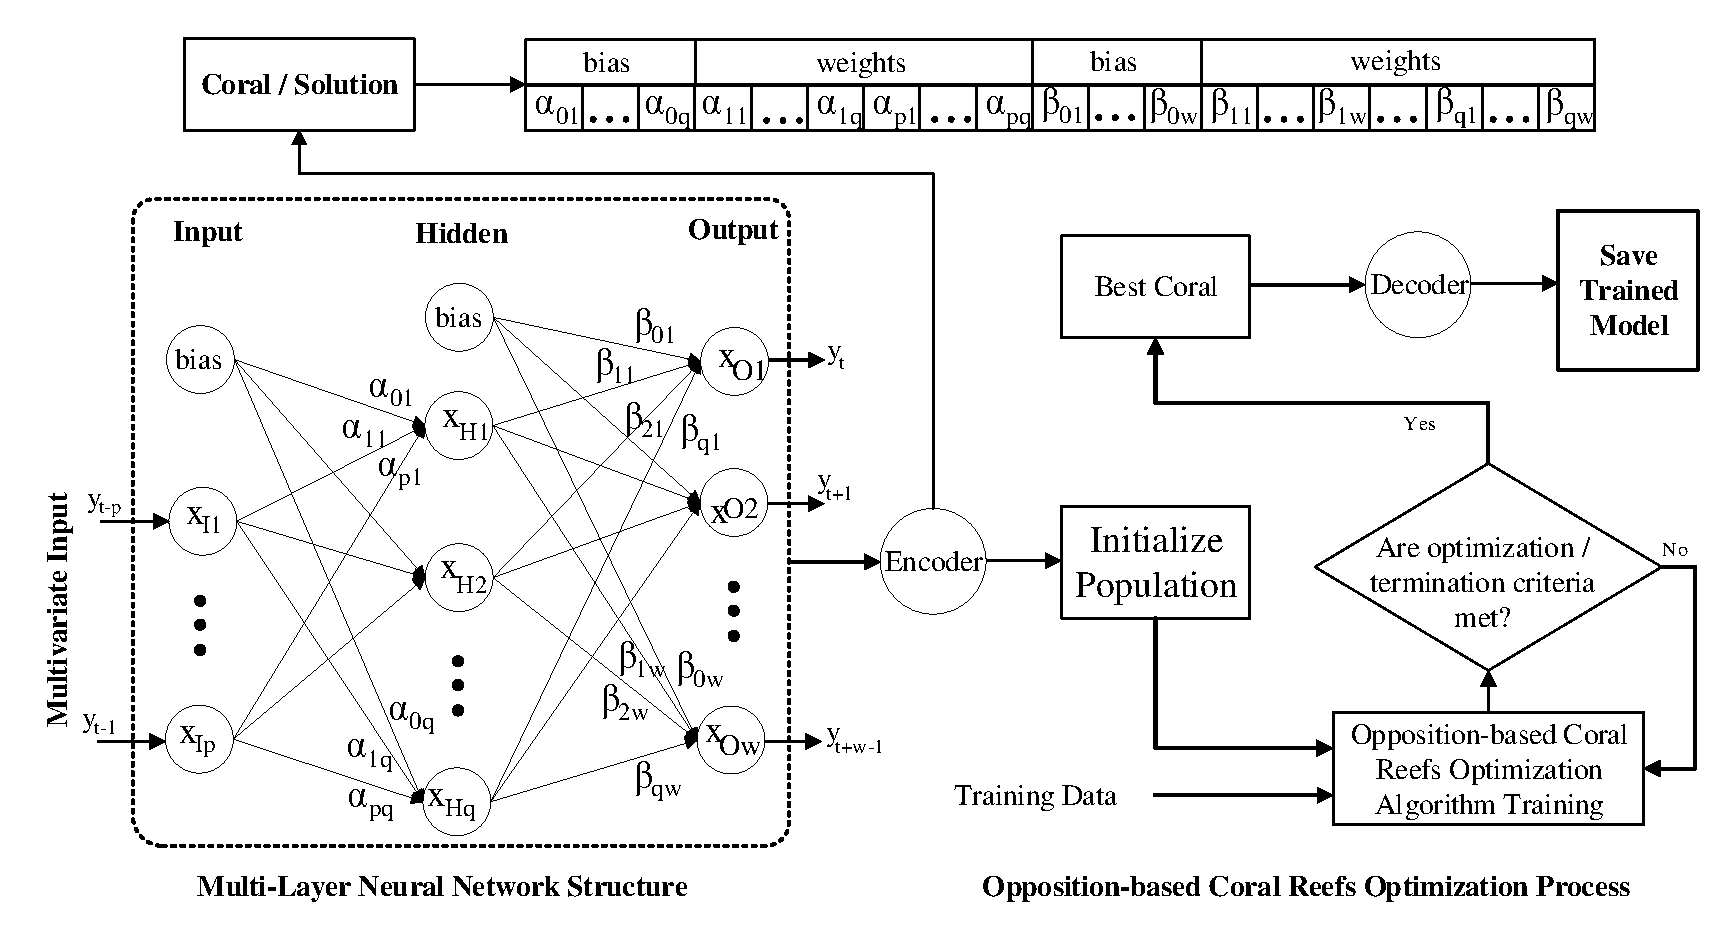
\includegraphics[width=1.0\textwidth =0cm 0cm 0cm 0cm, clip]{images/pdf/system/cro_training_final.pdf}
		\caption{OCRO-MLNN training process}
		\label{fig_ocro_training}
	\end{center}
\end{figure}

The learning process of OCRO-MLNN is illustrated by Fig.~\ref{fig_ocro_training}. To obtain the multivariate input, raw data is preprocessed by the following steps.

\begin{enumerate}
	\item Firstly, a time series data is scaled into the range of $[0, 1]$. 
	\item Secondly, time series data is transformed to supervised data using sliding method with window width $k$, where $k$ is prior observations before time $t$ used to predict the observation at $t$. 
	\item Finally, all metric types are grouped into multivariate input. Encoder and decoder are two important components in Fig.~\ref{fig_ocro_training}. In which, encoder encodes NN weights and biases into our domain solution (i.e. coral presented as real-value vector). Decoder decodes corals back into NN weights and biases. 
	\item In order to avoid long training time, a termination criterion is designed for earlier-stopping after the number of epochs (training cycles) is predefined or after achievement of error goal. 
\end{enumerate}

Algorithm~\ref{MLNN_OCRO} describes the MLNN operation with OCRO. The parameters are shown in Table~\ref{table:ocro_paras}.

%\begin{algorithm}[ht!]
%	\caption{Combination of MLNN with OCRO}\label{MLNN_OCRO}
%	\hspace*{\algorithmicindent} \textbf{Input:} 
%	\textbf{ $g_{max}$, $N$, $M$, $\rho_{o}$, $F_{b}$, $F_{a}$, $F_{d}$, $k$, $\tau$ }\\
%	\hspace*{\algorithmicindent} \textbf{Output:} The best coral - $C_{best}$
%	\begin{algorithmic}[1]
%		\State Normalize all current resource time series of M type of resource consumption: $r_1(t),..,r_M(t)$
%		\State Initialize sliding window with p consecutive points as the inputs $(X_1(t-1),..., X_1(t-p)),..., (X_M(t-1),..., X_M(t-p))$ and the next observation $X_1(t), ..., X_M(t+w-1)$ as the outputs (t = 1,2,...,n)
%		\State Group all column inputs data of M type resource into a unique multivariate one  $X(t) = [ X_1(t-1), ..., X_1(t-p), ..., X_M(t-1), ..., X_M(t-p) ]$
%		\State Training MLNN by OCRO algorithm from step 5 to 39.
%		\State Initializing reef space includes $N$ x $M$ square grid, assign some squares to be occupied by corals with respect to rate $\rho_{o}$ = free/occupied
%		\State $C_{best} \gets$ The best coral in reef based on their health
%		\State $iters\_count \gets 0$
%		
%  		\For{\texttt{i = 0 to $g_{max}$}}
%  		
%	     		%\State \textbf{Broadcast Spawning}
%	     		\State $larvaes \gets \emptyset$
%	     		\State $C_{broadcast} \gets$ Take out a fraction $F_{b}$ of coral reefs.
%	     		\State $C_{brooding} \gets$ Corals in reef, exclusive in $C_{broadcast}$
%	     		
%	     		\For{$C_{1}, C_{2}$ \texttt{in} $C_{broadcast}$}
%	        			\State $larva \gets$ \texttt{Crossover($C_{1}, C_{2}$)}
%	        			\State $larvaes$\texttt{.append($larva$)}
%	     		\EndFor    
%	     		
%	     		%\State \textbf{Brooding}
%	     		\For{$C_{b}$ \texttt{in} $C_{brooding}$}
%	        			\State $larva \gets$ \texttt{Mutation($C_{b}$)}
%	        			\State $larvaes$\texttt{.append($larva$)}
%	     		\EndFor   
%
% 	     		%\State \textbf{LarvaeSettting}
%	     		\For{$larva$ \texttt{in} $larvaes$}
%	        			\For{\texttt{j = 0 to $k$}}
%	        				\State square $\gets$ Select a random square in reef
%	           			\If{ square is empty \texttt{or} $f(larva) \geq f(square)$}
%	              			\State square $\gets larva$ 
%	              			\Break
%	           			\EndIf
%	        			\EndFor
%	     		\EndFor
%	     
%	     		%\State \textbf{Reproduction}
%	     		\State $C_{duplicate} \gets$ A fraction $F_{a}$ of healthy corals
%	     		\State $C_{depredation} \gets$ A fraction $F_{d}$ of worse health corals
%	     		\State Run step 18 to 23 (Larvaes setting) for $C_{duplicate}$
%      		
%      			%\State \textbf{Depredation}
%	     		\For{$C_{d}$ \texttt{in} $C_{depredation}$}
%	        			\State $C_{op} \gets L_{b} + U_{b} - C_{best} + r\times(C_{best} - C_{d})$
%	        			\If{$f(C_{op}) \geq f(C_{d})$}
%	           			\State \texttt{Replace $C_{d}$ by $C_{op}$}
%	        			\Else
%	           			\State \texttt{Free space at $C_{d}$ position}
%	        			\EndIf
%	     		\EndFor
%     		
%     			\If{ $C_{best}$ doesn't change after $\tau$ iterations}
%   				\State $iters\_count \gets iters\_count$ + 1
%    				\State $C_{best} \gets$ The best coral in reef based on their health
%    				\If{ $C_{best}$ doesn't change and $iters\_count \geq \tau$}
%	         			\State Restart searching and keep $C_{best}$
%	      				\State $iters\_count \gets 0$
%      				\EndIf
%    			\EndIf
%    			
%     		\EndFor
%		\State Return $C_{best}$
%	\end{algorithmic}
%\end{algorithm}

\begin{algorithm}
	\caption{OCRO-MLNN forecasting model}\label{MLNN_OCRO}
	\hspace*{\algorithmicindent} \textbf{Input:} 
	\textbf{ $g_{max}$, $N$, $M$, $\rho_{o}$, $F_{b}$, $F_{a}$, $F_{d}$, $k$, $\tau$ }\\
	\hspace*{\algorithmicindent} \textbf{Output:} $C_{best}$ the best coral in reef based on their health.
	\begin{algorithmic}[1]
		\State Initializing reef space includes $N$ x $M$ square grid, 
		\Statex assign some squares to be occupied by corals with respect to rate $\rho_{o}$ = free/occupied, 
		\Statex find the $C_{best}$ and $n_{iters} \gets 0$

  		\For{i = 0 to $g_{max}$}
  		
	     		%\State \textbf{Broadcast Spawning}
	     		\State $larvaes \gets \emptyset$
	     		\State $C_{broadcast} \gets$ take out a fraction $F_{b}$ of coral reefs.
	     		\State $C_{brooding} \gets$ Corals in reef, exclusive in $C_{broadcast}$
	     		
	     		\For{$C_{1}, C_{2}$ in $C_{broadcast}$}
	     			\State Crossover $C_{1}$ and $C_{2}$ to create new larva and then add that larva to $larvaes$
	     		\EndFor    
	     		
	     		%\State \textbf{Brooding}
	     		\For{$C_{b}$ in $C_{brooding}$}
	     			\State Mutation $C_{b}$ to create new larva and then add that larva to $larvaes$
	     		\EndFor   

 	     		%\State \textbf{LarvaeSettting}
	     		\For{$larva$ in $larvaes$}
	        			\For{j = 0 to $k$}
	        				\State square $\gets$ select a random square in reef
	           			\If{ square is empty or $f(larva) \geq f(square)$}
	              			\State square $\gets larva$ 
	              			\Break
	           			\EndIf
	        			\EndFor
	     		\EndFor
	     
	     		%\State \textbf{Reproduction}
	     		\State $C_{duplicate} \gets F_{a}$ fraction of healthy corals
	     		\State $C_{depredation} \gets F_{d}$ fraction of worse health corals
	     		\State Run step 11 to 16 (Larvaes setting) for $C_{duplicate}$
      		
      			%\State \textbf{Depredation}
	     		\For{$C_{d}$ in $C_{depredation}$}
	        			\State $C_{op} \gets L_{b} + U_{b} - C_{best} + r \cdot (C_{best} - C_{d})$
	        			\If{$f(C_{op}) \geq f(C_{d})$}
	           			\State Replace $C_{d}$ by $C_{op}$
	        			\Else
	           			\State Free space at $C_{d}$ position
	        			\EndIf
	     		\EndFor
     			
     			\State Find the best current coral $C'_{best}$
     			\If{ $C'_{best}$ is the same as $C_{best}$}
   				\State $n_{iters}$ $\gets$ $n_{iters}$ + 1 
    				\If{$n_{iters} \geq \tau$}
	         		\State Restart searching, keep $C_{best}$ and $n_{iters} \gets 0$
      			\EndIf
    			\EndIf
    			
     		\EndFor
		\State Return $C_{best}$
	\end{algorithmic}
\end{algorithm}

\begin{table}[!h]
\begin{center}
\begin{tabular}{ C{1.5cm}| L{14cm}  } 
%\hline
\textbf{Name} & \textbf{Description} \\ 		\hline
$g_{max}$ & Maximum number of generations \\ 	%\hline
$N \times M$ & Number of square grids in reef \\ 		%\hline
$\rho_{o}$ & The rate between free/occupied squares in reef at the beginning of this algorithm \\ 		%\hline
$F_{b}$ & The fraction of broadcast spawners with respect to the overall amount of existing corals \\ 	%\hline
$1 - F_{b}$ & The fraction of corals that will reproduce by brooding \\ 	%\hline
$F_{a}$ & A fraction of reef that will duplicates itself \\ 				%\hline
$F_{d}$ & A fraction of worse health corals will be depredated.  \\ 		%\hline
$k$ & Number of attempts for a larva to set in the reef \\ 				%\hline
$\tau$ & Number of iters before restarting the algorithm \\ 					%\hline
\end{tabular}
\end{center}
\caption{Opposition-Based Coral Reefs Optimization (OCRO) parameters}
\label{table:ocro_paras}
\end{table}

\section{Experiments and evaluations}
\label{experiments}

\subsection{Evaluation approach}
Under assumption of the same datasets, settings and testing environment, two experiment groups are carried out to evaluate the proposed OCRO-MLNN model, covering:

\begin{enumerate}
	\item Evaluating the proposed model on both univariate and multivariate data of different datasets.
	\item For each test, prediction accuracy, run-time and model stability among various NN models are compared with our OCRO-MLNN model. 
\end{enumerate}

Other NN models used for comparison include traditional MLNN and its variances with optimization techniques such as GA-MLNN, PSO-MLNN, ABFO-MLNN, CRO-MLNN, traditional RNN and the state-of-the-art LSTM.

\subsubsection{Datasets}
\label{dataset}

\paragraph{\textbf{Univariate data.}} Univariate data used in our experiments are two real and well-known datasets, covering:

\begin{itemize}
	\item "Internet traffic data (in megabytes)"~\citep{ref_cortez} collected from a private Internet Service Provider (ISP) with distributed centers in 11 European cities (in short from here EU dataset). The dataset corresponds to a transatlantic link and was collected from June 7th to 11:17 hours on July 31st, 2005 in five minutes intervals. 
	\item The second dataset (called WorldCup98, in short from here WC dataset) contains request numbers (in thousands) to servers in world-cup season between April 30th, 1998 and July 26th, 1998. The dataset is processed into five minutes intervals in our work.
\end{itemize}

\paragraph{\textbf{Multivariate data.}} Multivariate data used in our experiments are gathered by Google from their production data center clusters (called Google trace dataset, in short from here Google dataset). The log records come from approximately 12000 servers for one month~\citep{ref_google_trace} and~\citep{reiss2011google}. Based on our prior analysis presented in~\citep{ref_thieu}, we select both resource usages, which are CPU and memory metric as multivariate inputs for our proposed models. The dataset also was further processed into five minutes intervals in the experiments. Visualization of both data type is illustrated in Fig.~\ref{dataset_visual}.

\begin{figure}[!ht] 
  \begin{minipage}[b]{0.48\linewidth}
    \centering
    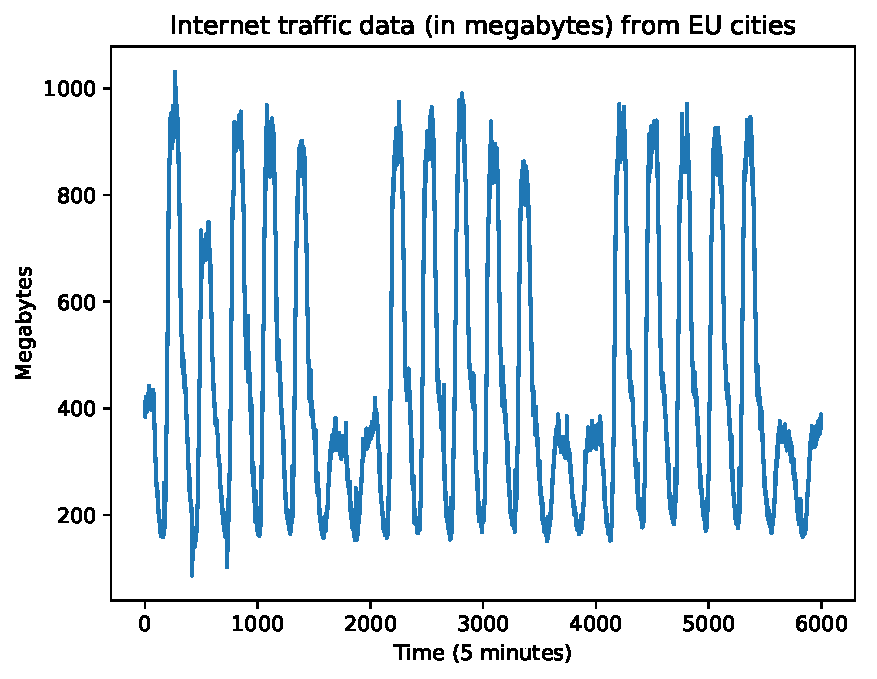
\includegraphics[width=0.9\linewidth]{images/pdf/data/internet_traffic_eu_5m.pdf} 
  \end{minipage}
  \begin{minipage}[b]{0.48\linewidth}
    \centering
    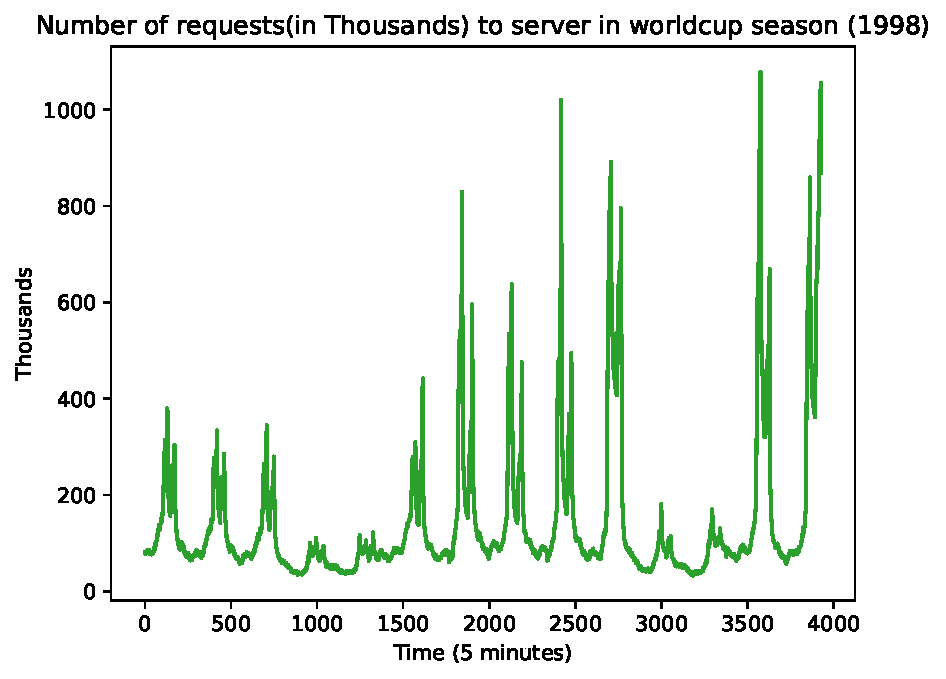
\includegraphics[width=0.9\linewidth]{images/pdf/data/worldcup98_5m.pdf} 
  \end{minipage} 
  
  \begin{minipage}[b]{0.48\linewidth}
    \centering
    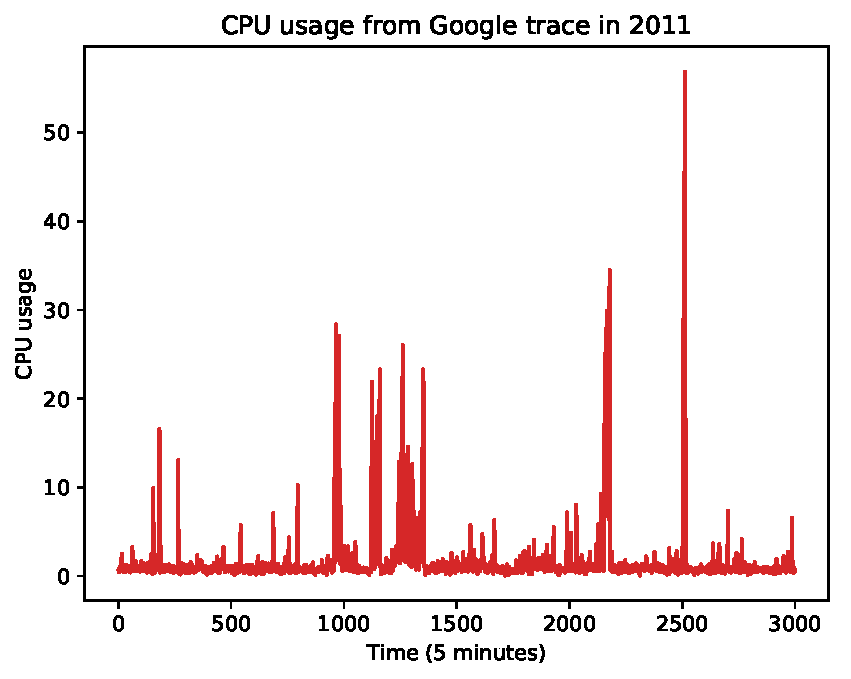
\includegraphics[width=0.9\linewidth]{images/pdf/data/google_cpu_5m.pdf} 
  \end{minipage}%% 
  \begin{minipage}[b]{0.48\linewidth}
    \centering
    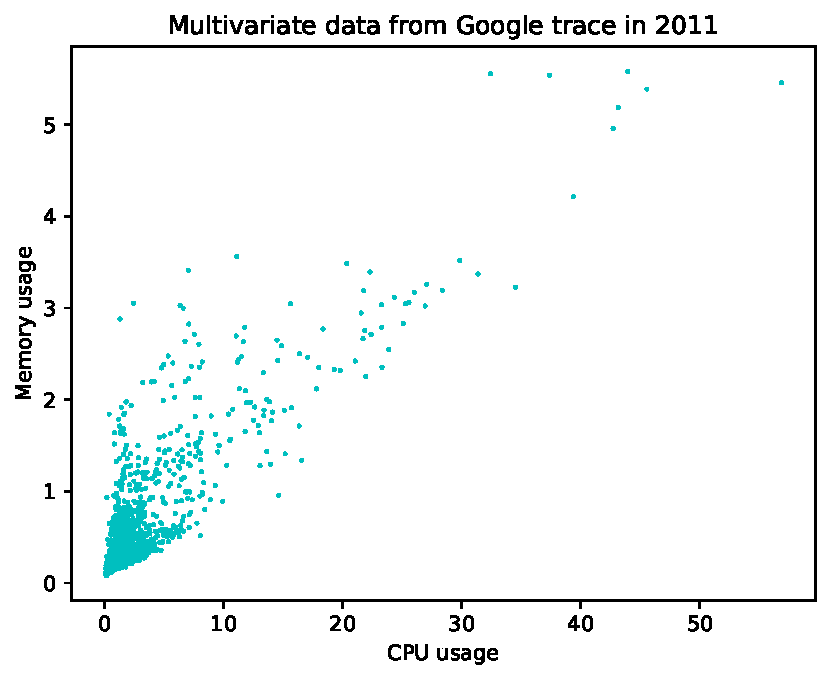
\includegraphics[width=0.89\linewidth]{images/pdf/data/cpu_ram.pdf} 
  \end{minipage} 
  
  \caption{Dataset visualizations: univariate data (upper row) and multivariate data (lower row)} 
  \label{dataset_visual} 
\end{figure}

\subsubsection{Measurement methods}
\label{measurement_methods}

\paragraph{\textbf{Accuracy.}} In our work, Root Mean Square Error (RMSE) (Equation.~\ref{eq_rmse}) is used mainly to evaluate error between predicted and ground true value. It is also employed as the fitness function in GA, PSO, ABFO, and as the health function in CRO and OCRO. However, for objectiveness, other metrics such as Coefficient of Determination ($R^2$), Mean Absolute Error (MAE), Mean Absolute Percentage Error (MAPE), and Symmetric Mean Absolute Percentage Error (SMAPE) are also used to comparison goal. The mathematical formulations of those metrics are presented in Equation.~\ref{eq_r2}, Equation.~\ref{eq_mae}, Equation.~\ref{eq_mape} and Equation.~\ref{eq_smape} respectively.

%\scriptsize
 \small

\begin{equation} \label{eq_rmse}
fitness = health = RMSE = \sqrt{ \frac{\sum_{i=1}^N (forecast(i) - actual(i))^2 }{N} }
\end{equation}

\begin{equation} \label{eq_r2}
R^2 = 1 - \displaystyle \frac{ \sum\limits_{i=1}^N \Bigl( actual(i) - forecast(i) \Bigr)^2} { \sum\limits_{i=1}^N \Bigl( actual(i) - \frac{1}{N} \sum\limits_{j=1}^N actual(j) \Bigr)^2  }
\end{equation}

\begin{equation} \label{eq_mae}
MAE = \frac{\sum_{i=1}^N|forecast(i) - actual(i)|}{N}
\end{equation}

\begin{equation} \label{eq_mape}
MAPE = \frac{100\%}{N} \sum_{i=1}^N \left\lvert \frac{actual(i) - forecast(i)}{actual(i)} \right\rvert
\end{equation}

\begin{equation} \label{eq_smape}
SMAPE = \frac{100\%}{N} \sum_{i=1}^N \frac{ |forecast(i) - actual(i)| }{ (|actual(i)| + |forecast(i)|)/2  }
\end{equation}
\normalsize

\paragraph{\textbf{Runtime.}} The proposed model OCRO-MLNN is also compared with other models in runtime performance-wise (speed) aspect. Currently, RNN and particularly LSTM are state-of-the-art for time-series prediction models. The fact is their complicated structure 
%\GN{so It's difficult to implement - NO when we can use wrapper like Keras} 
and training runtime often is long. Hence, it is desired to have a model with at least comparable good prediction performance but less expensive on computational requirement. 
%It's also the vital element for such a problem required faster time. We not only want to prove our model with the same results, even better in some cases in comparison with the state-of-the-art model, but also prove our model can be better in complexity of time aspect. 
The runtime comparison in our experiments is done according to three factors: 

\begin{itemize}
	\item $t_e$ is the average time for 1 epoch (second/epoch).
	\item $t_p$ is time to predict test data (in second). 
	\item $t_s$ is the total time of all system processing (preprocessing, training and testing) The unit is also second. 
\end {itemize}

Because each model has different epoch configuration, $t_e$ can give the most objective insight into the model complexity instead of the total time of training process. However, $\boldsymbol{t_s}$ is definitively the decisive factor that everyone cares about the most. 

\subsubsection{Settings parameters for algorithms and models}
\label{para_settings}
%- MLNN (1 Hidden Layer)
%- RNN (1 HL)
%- LSTM (1 HL, 2 HL) 
%- GA-MLNN	
%- CRO-MLNN 

As described above, OCRO-MLNN is validated against other modes such as MLNN, GA-MLNN, PSO-MLNN, ABFO-MLNN, CRO-MLNN, RNN and LSTM. 

\begin{itemize}
\item MLNN part in the all models listed above are is configured with the same structure configuration (three layers (input, hidden and output layer)). The architecture is similar to typical topology of one RNN/LSTM block~\citep{ref_xiaolei}. 
\item Input size $p$ = $k \cdot m$, where $k$ is sliding window and $m$ is the number of metric types in dataset (i.e. $m=1$ for univariate and $m>1$ for multivariate). The number of neurons in the hidden layer is set by $q=5$ for all models. The output size $w=1$. 
\item In RNN and LSTM models, NN is composed from one input layer, one RNN/LSTM block and one output layer with similar parameter settings. Activation function used in the models is ELU as described above in Section~\ref{mlnn}.
\item To be fair in all test, the population size $p_s$ and maximum number of generations $g_{max}$ of meta-heuristics such as GA, PSO, ABFO, CRO and OCRO is set to the same 200 and 700 respectively~\citep{ref_thieu}. The number of generations of MLNN is set to 5000 because of the slow convergence of BP algorithm. Meanwhile, the number of the epoch in RNN and LSTM is 1000 to avoid the massive timing cost.
\end{itemize}

Besides above-described common specifications for fairness testing, the following settings are applied to algorithms for their best tested performance.

\begin{itemize}
\item For GA, probability of two individuals exchanging crossovers $p_c$ is set to $0.95$ and probability of individual mutation $p_m$ is set to $0.025$ based on our prior work~\citep{ref_thieu}. 
\item For PSO, based on~\citep{ref_shi2001particle}, inertia factor $w$ is set linearly reducing with iteration from $0.9$ to $0.4$, cognitive learning rate $c1 = c2 = 1.2$.
\item For ABFO, according to our prior experiment~\cite{ref_thieu}, swimming length is set $N_s=4$, probability for eliminate bacteria $P_e=0.25$, parameters used to control and adjust split and dead criterion $N_{split}=30$, $N_{adapt}$ = 5, step size at the beginning of process $C_s= 0.1$ ($U_b - L_b$), step size at the end of process $C_e=0.00001$ ($U_b - L_b$), where $U_b$ and $L_b$ are referred to the upper and lower bound of the variables.
\item For CRO, based on~\citep{ref_salcedo_sanz1}, initial free/occupied square ($p_{o}$) should be enough to allow new poorer solutions in order to have enough survival probability, so $p_{o}$ is set by 0.4. The maximum number of generations $g_{max}$ = 1000. The depredation probability $P_{d}$ linearly increases from 0 as initial value to 0.1 at the end of algorithm operation. A high value of corals applying broadcast spawning is needed in order to ensure an efficient exploration of the search space. On the other hand, a small value of brooding and asexual reproduction is advisable, therefore we set $F_{b}$ = 0.9 and $F_{a}$ = 0.1. 
We also find out that with 250 corals in reef and number $k$ of attempts for a larva is set in the reef equals to 3 that is good for our problems~\citep{ref_salcedo_sanz1}.
\item For OCRO, most of parameters are set similar to CRO except broadcast spawning fraction $F_{b}$, depredation fraction $F_{d}$, and $\tau$, which is the number of iterations before restarting algorithm. In order to make opposition based on searching work efficiently, a high fraction of corals is supposed to be applied by this technique. But on the other hand, the number of corals in reef also need to be stable during the training. So, with a small change in fraction of broadcast spawning, and budding that helps more larva can be created during sexual reproduction phase.
	\begin{itemize} 
		\item For $\tau$, it must be small enough to prevent premature convergence but also not too small that may cause algorithm only working on global searching and cannot converge to optimal solution. 
		\item Our proposed $F_{b}$ is set to 0.8 (more corals for budding that is one coral create one larva, while in broadcast spawning we need a couple to have a new larva).
		\item $F_{d}$ = 0.3 and $\tau$ = 55 are supposed to be proper after testing on our datasets.
	\end{itemize}
\end{itemize}

\subsection{Experiment results}
\label{results_discussion}

\subsubsection{Univariate data}
\paragraph{\textbf{Prediction accuracy.}} Table~\ref{table:uni_forecast} describes obtained experiment results with above-mentioned models on two datasets. The overall evaluation is as follows.

\begin{itemize}
	\item In general, MLNN and ABFO-MLNN models did not bring performance well in accuracy mean as comparison with the rest. 
	\item With the EU dataset, our proposed OCRO-MLNN performances has the best with (RMSE, MAE) = (15.535, 11.058) and (15.381, 10.918) for $k = 2$ and $k = 5$, respectively. 	
	\item LSTM get the best results with index of $R^{2}$, which are 0.9958 and 0.9959 for $k = 2$ and $k = 5$, respectively. In comparison with CRO-MLNN ($R^{2}$ = 0.9954 for $k = 2$ and 0.9950 for $k = 5$) and OCRO-MLNN ($R^2$ = 0.9955 for $k = 2$ and 0.9956 for $k = 5$), LSTM is just slightly better. 
	\item With the WC dataset, for all four metrics $R^2$, MAE, MAPE and SMAPE with sliding window $k = 5$, the obtained results with OCRO-MLNN are remarkable when get the best accuracies that marked in bold numbers in the table. 
\end{itemize}


%	 althought RNN and LSTM get good results with MAPE (RNN's MAPE = 4.7003 which is the best) but in other measurement terms they all get worse with RMSE around 0.0163 and $R^{2}$ around 0.990, while CRO-MLNN's RMSE = 0.0134 ($k = 5$) and OCRO-MLNN's results are still considered work well for all measurement. 

Table~\ref{table:uni_forecast} shows that OCRO-MLNN not only improves the original CRO-MLNN but also gets better accuracy as compared with LSTM. Fig.~\ref{predict_eu_sliding2} and {Fig.~\ref{predict_wc_sliding5} express the prediction results to illustrate the gained data. 
% ======================= Table accuracy ================================

% fit-width table
\begin{table}[!h]
	\caption{RMSE, MAPE and $R^2$ comparison (sliding window $k$ = 2 and $k$ = 5; univariate datasets)}
	\label{table:uni_forecast}
	\centering
	\begin{adjustbox}{width=\textwidth}
%	\begin{sideways}
		\begin{tabular}{| c | c | c | c | c | c | c | c | c | c | c | c |}%
			\hline
			\multirow{2}{*}{Data} & \multirow{2}{*}{Model} & \multicolumn{2}{c|}{$R^2$} & \multicolumn{2}{c|}{RMSE} & \multicolumn{2}{c|}{MAE} & \multicolumn{2}{c|}{MAPE}  & \multicolumn{2}{c|}{SMAPE} \\ \cline{3-12}
   				& & $k$ = 2 & $k$ = 5 & $k$ = 2 & $k$ = 5 & $k$ = 2 & $k$ = 5 & $k$ = 2 & $k$ = 5 & $k$ = 2 & $k$ = 5 \\ [0.5ex] 
			\hline
			\primitiveinput{table/table_uni_forecast}
			\hline
		\end{tabular}
%	\end{sideways}
	\end{adjustbox}
\end{table}


%% rotated and fit-heigh table 
%\begin{table}
%	\caption{RMSE, MAPE and $R^2$ comparison between our proposed OCRO-MLNN and other models with sliding window k = 2 and k = 5 (univariate dataset)}
%	\label{table:uni_forecast_rotate}
%	\centering
%	\begin{adjustbox}{height=\textheight}
%	\begin{sideways}
%		\begin{tabular}{| c | c| c | c | c | c | c | c | c | c | c | c |}%
%			\hline
%			 \multirow{2}{*}{Data} & \multirow{2}{*}{Model} & \multicolumn{2}{c|}{$R^2$} & \multicolumn{2}{c|}{RMSE} & \multicolumn{2}{c|}{MAE} & \multicolumn{2}{c|}{MAPE}  & \multicolumn{2}{c|}{SMAPE} \\ \cline{3-12}
%   				& & k = 2 & k = 5 & k = 2 & k = 5 & k = 2 & k = 5 & k = 2 & k = 5 & k = 2 & k = 5 \\ [0.5ex] 
%			\hline
%			\primitiveinput{table/table_uni_forecast}
%			\hline
%		\end{tabular}
%	\end{sideways}
%	\end{adjustbox}
%\end{table}

\begin{figure}[!ht] 
  \begin{minipage}[b]{0.33\linewidth}
    \centering
    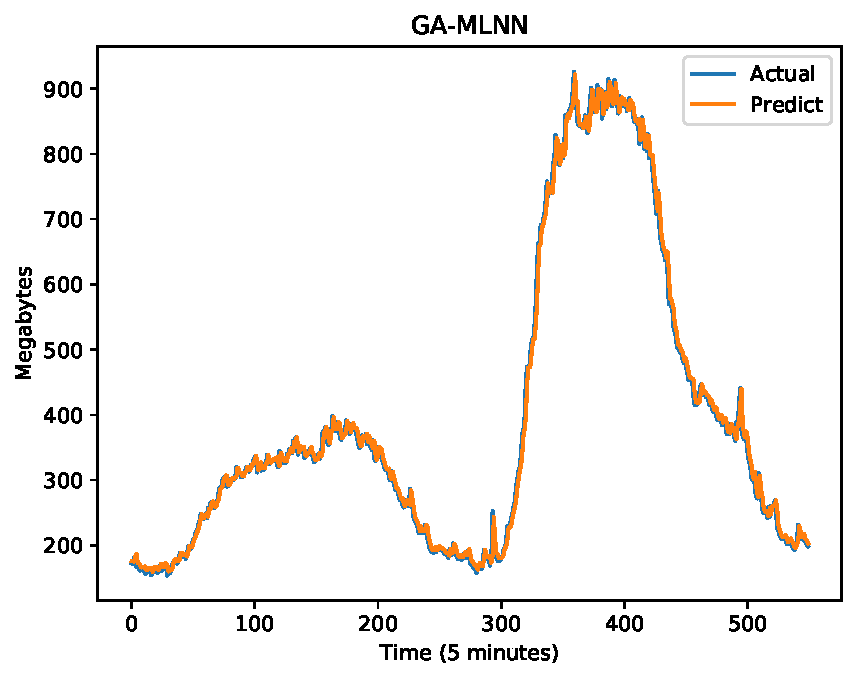
\includegraphics[width=0.9\linewidth]{images/pdf/predict/k2/eu_k2_ga_mlnn.pdf} 
  \end{minipage}
  \begin{minipage}[b]{0.33\linewidth}
    \centering
    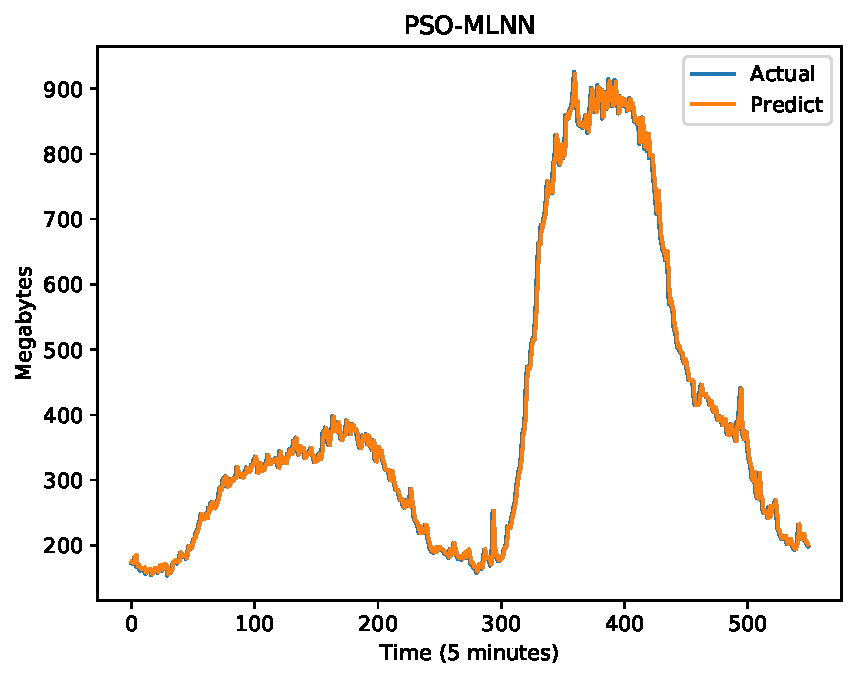
\includegraphics[width=0.9\linewidth]{images/pdf/predict/k2/eu_k2_pso_mlnn.pdf} 
  \end{minipage} 
  \begin{minipage}[b]{0.33\linewidth}
    \centering
    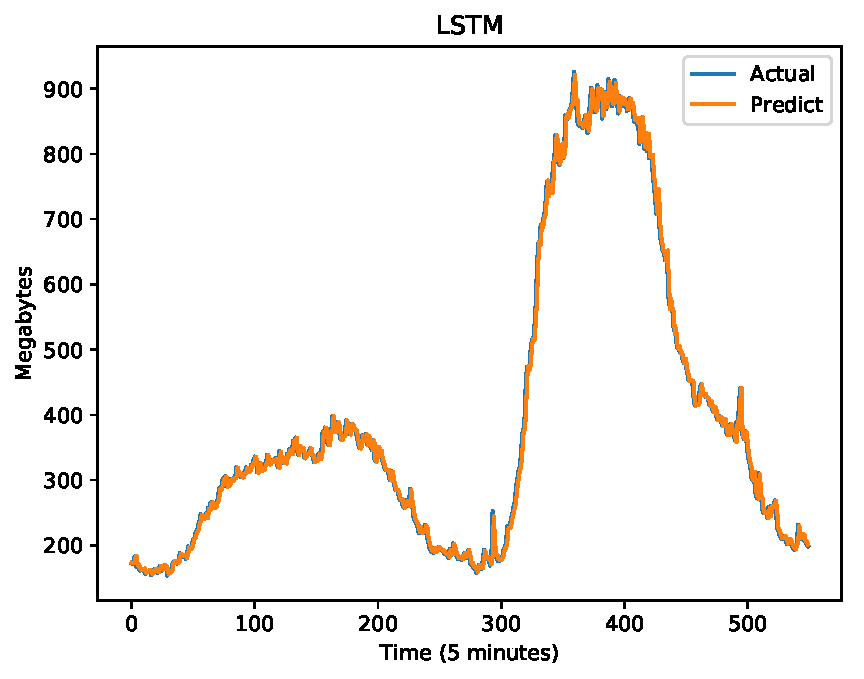
\includegraphics[width=0.9\linewidth]{images/pdf/predict/k2/eu_k2_lstm.pdf} 
  \end{minipage} 
  
   \begin{minipage}[b]{0.33\linewidth}
    \centering
    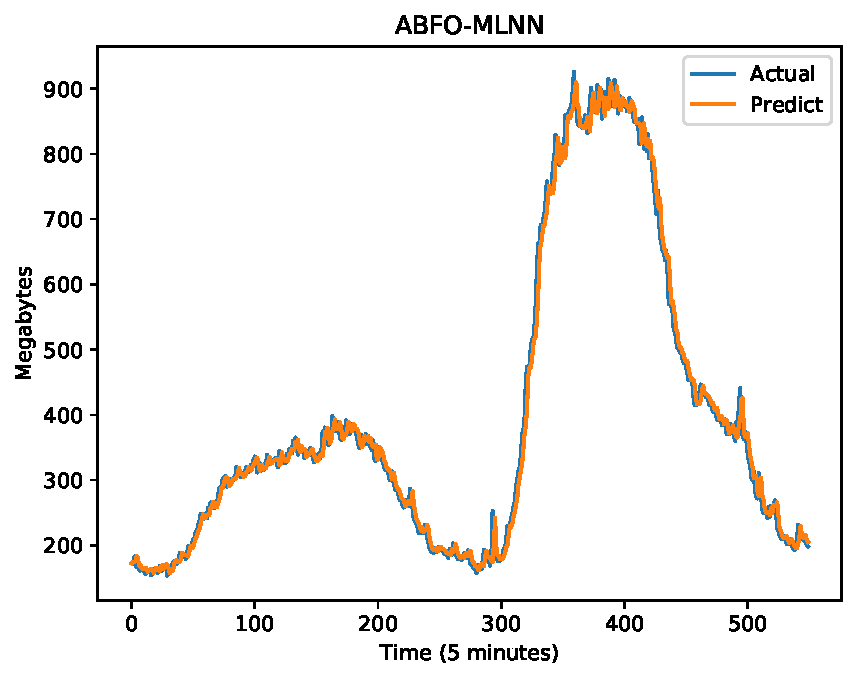
\includegraphics[width=0.9\linewidth]{images/pdf/predict/k2/eu_k2_abfo_mlnn.pdf} 
  \end{minipage}
  \begin{minipage}[b]{0.33\linewidth}
    \centering
    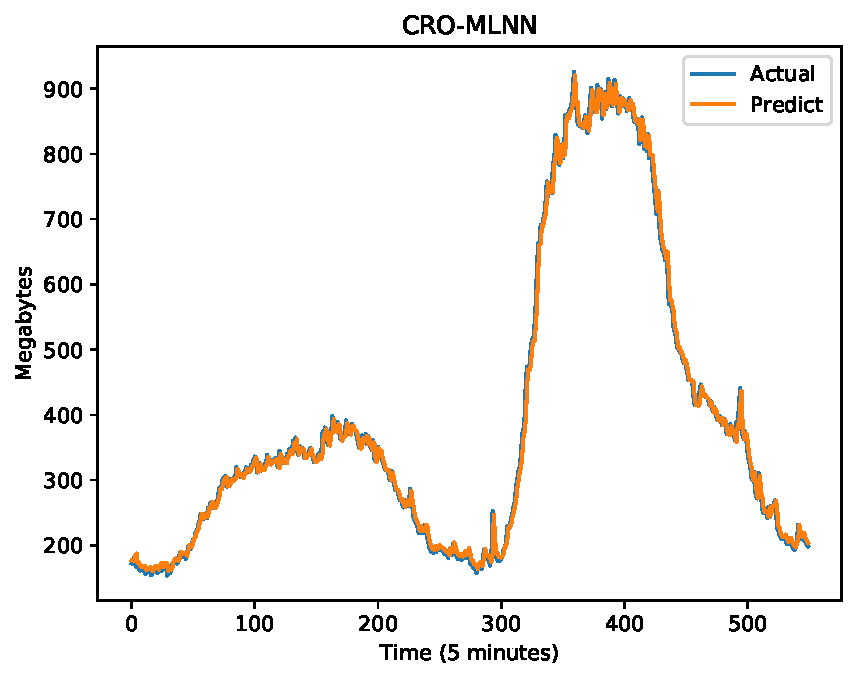
\includegraphics[width=0.9\linewidth]{images/pdf/predict/k2/eu_k2_cro_mlnn.pdf} 
  \end{minipage} 
  \begin{minipage}[b]{0.33\linewidth}
    \centering
    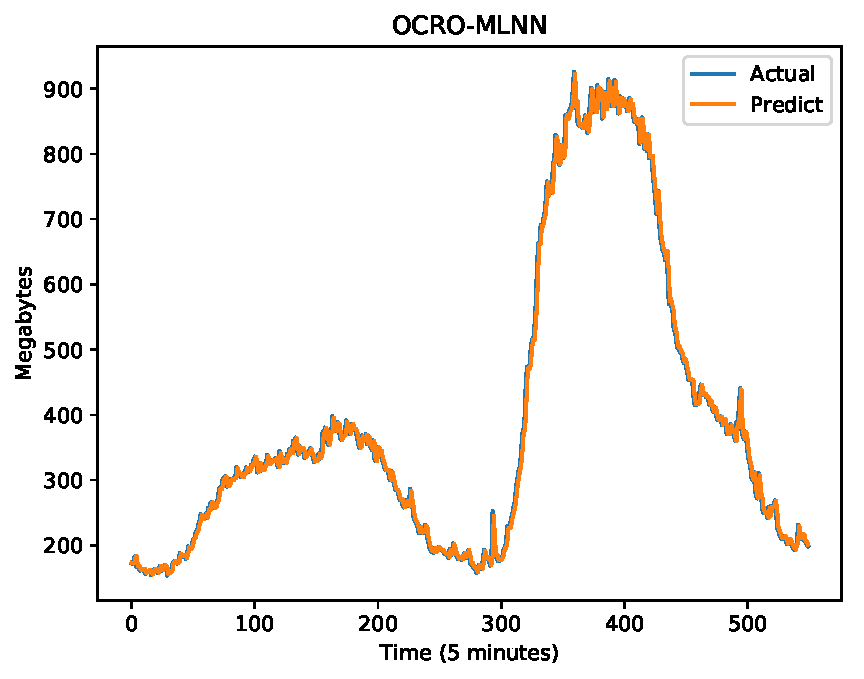
\includegraphics[width=0.9\linewidth]{images/pdf/predict/k2/eu_k2_ocro_mlnn.pdf} 
  \end{minipage} 
  
  \caption{Comparison of OCRO-MLNN prediction with other models (sliding window $k$ = 2; EU dataset)} 
  \label{predict_eu_sliding2} 
\end{figure}

\begin{figure}[!ht] 
  \begin{minipage}[b]{0.33\linewidth}
    \centering
    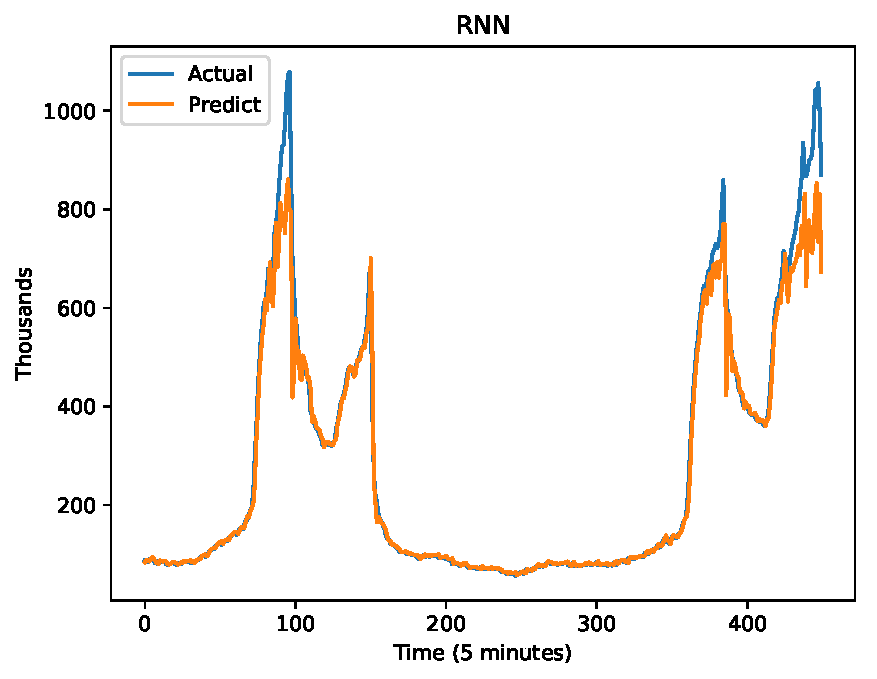
\includegraphics[width=0.9\linewidth]{images/pdf/predict/k5/wc_k5_rnn.pdf} 
  \end{minipage}
  \begin{minipage}[b]{0.33\linewidth}
    \centering
    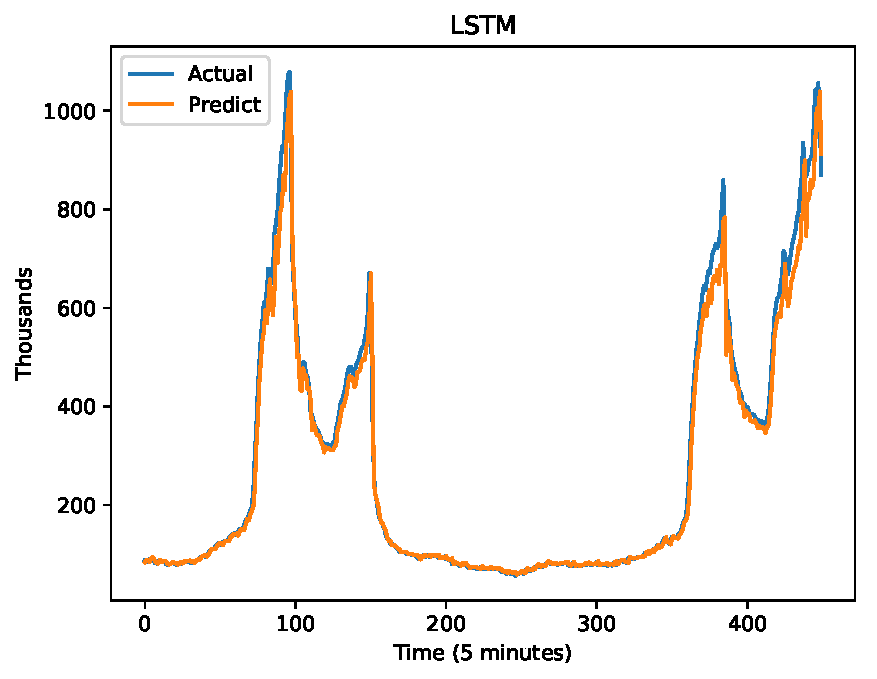
\includegraphics[width=0.9\linewidth]{images/pdf/predict/k5/wc_k5_lstm.pdf} 
  \end{minipage} 
  \begin{minipage}[b]{0.33\linewidth}
    \centering
    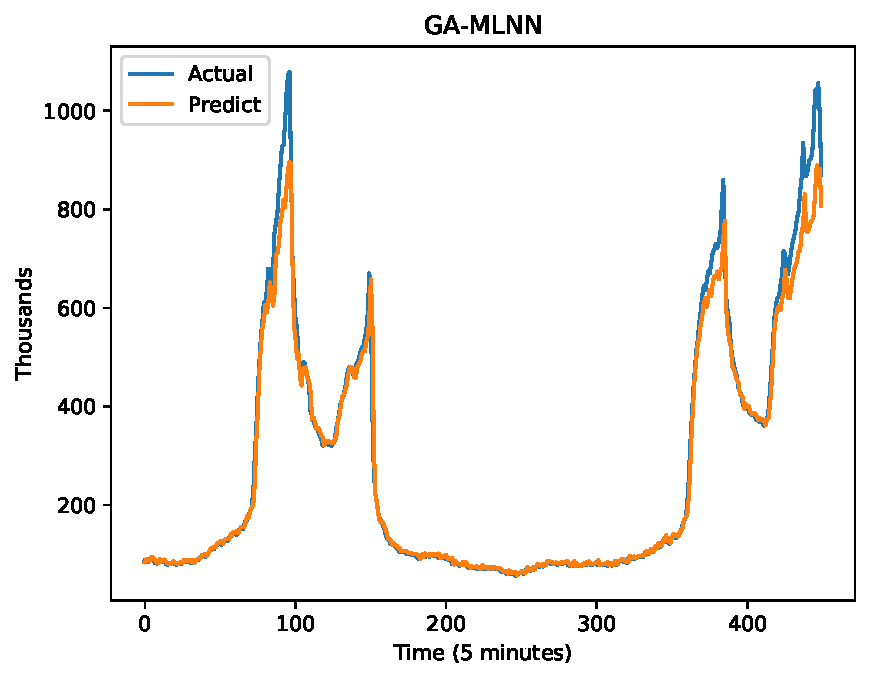
\includegraphics[width=0.9\linewidth]{images/pdf/predict/k5/wc_k5_ga_mlnn.pdf} 
  \end{minipage} 
  
  \begin{minipage}[b]{0.33\linewidth}
    \centering
    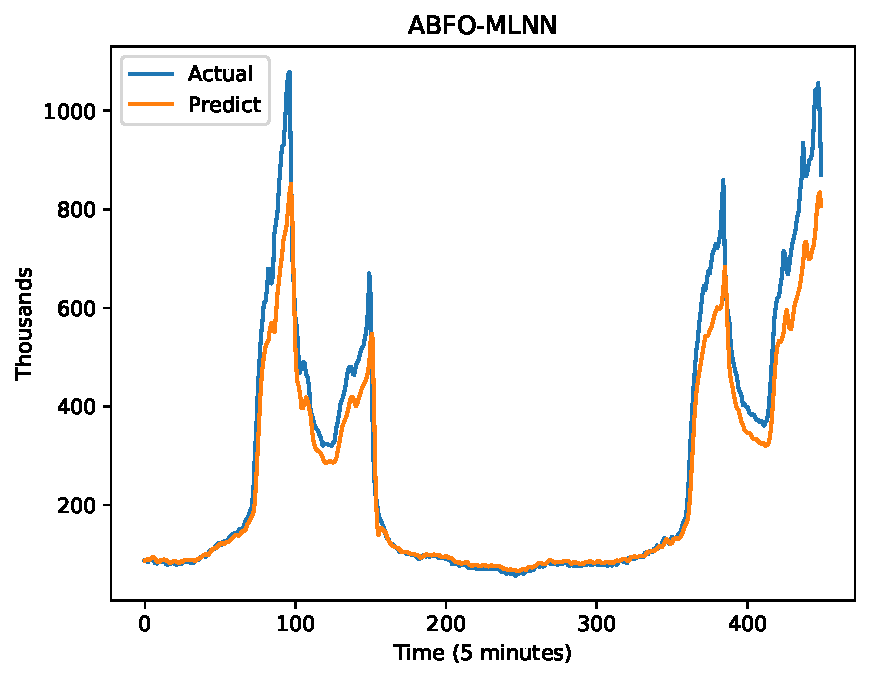
\includegraphics[width=0.9\linewidth]{images/pdf/predict/k5/wc_k5_abfo_mlnn.pdf} 
  \end{minipage}
  \begin{minipage}[b]{0.33\linewidth}
    \centering
    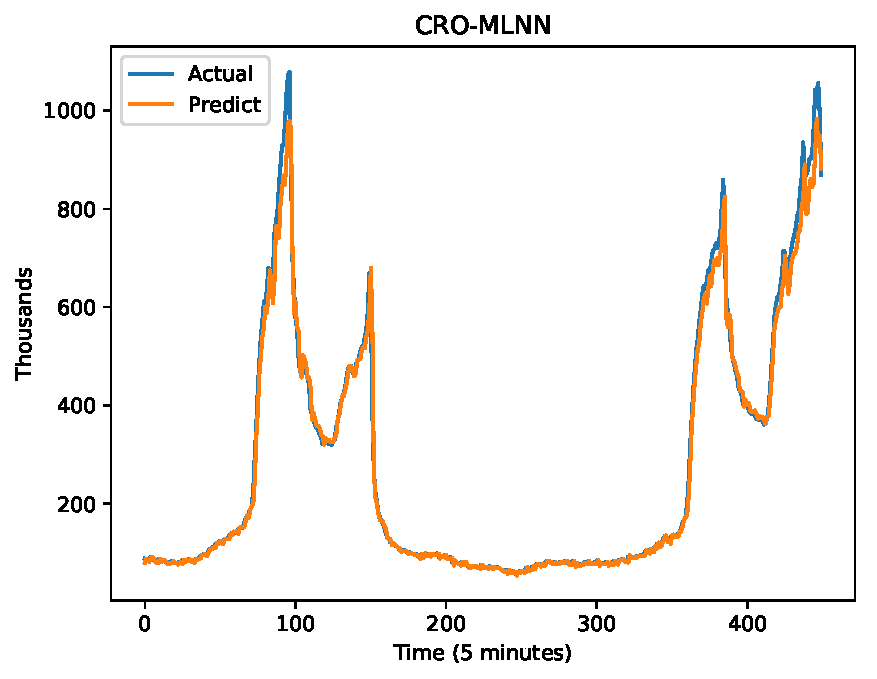
\includegraphics[width=0.9\linewidth]{images/pdf/predict/k5/wc_k5_cro_mlnn.pdf} 
  \end{minipage} 
  \begin{minipage}[b]{0.33\linewidth}
    \centering
    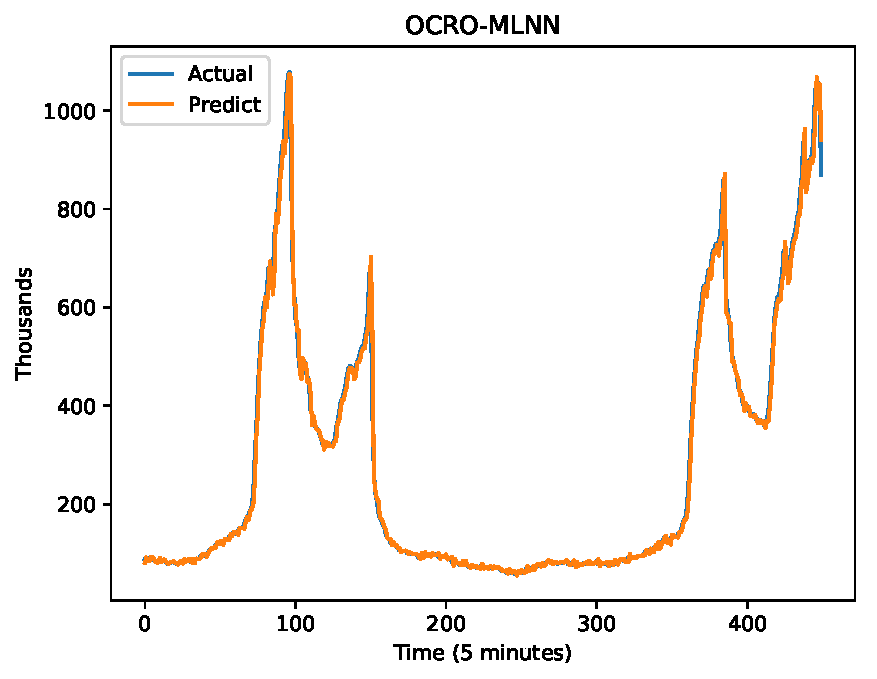
\includegraphics[width=0.9\linewidth]{images/pdf/predict/k5/wc_k5_ocro_mlnn.pdf} 
  \end{minipage} 
  \caption{Comparison of OCRO-MLNN prediction with other models (sliding window $k$ = 5; WC dataset)} 
  \label{predict_wc_sliding5} 
\end{figure}

\paragraph{\textbf{Runtime comparison.}} Table~\ref{table:uni_speed} shows runtime measurements of experiments. Note that epoch settings are described in detail in~\ref{para_settings}. There are some observations, which can be made as follows.

\begin{itemize}
\item RNN and LSTM have quite high runtime. For instance, with $k = 2$, RNN has $t_s$ = 2158.05 seconds and LSTM's $t_s$ is 1891.72 seconds. This issue causes by long epoch runtime. Concretely, with $k = 2$, RNN's $t_e$ is 2.1575 seconds and LSTM's $t_e$ is 1.8913 seconds. It is well-known that the models built from blocks have complicated structure, which is hard to optimize. Besides, the time cost also depends on hardware configuration of machines, which the models run on.
%Due to require of training epoch time is very large (for example, with $k = 2$, RNN's $t_e$ = 2.1575 seconds and LSTM's $t_e$ = 1.8913 seconds), then RNN and LSTM system's time become very large (with $k = 2$, RNN's $t_s$ = 2158.05 and LSTM's $t_s$ = 1891.72). This caused by the complicated structure of these  model and considered to be harmful to physical machine. 
\item Traditional MLNN's have significant small training time per epoch in comparison with others model. The disadvantage of MLNNs is its slow convergence, hence they need to train with more epochs. The overall effect is also longer time on train. 
%For the traditional MLNN's training time per epoch is significant small compare to others but slow convergence causes this model to need more time on training process. 
\item OCRO-MLNN and CRO-MLNN provide good runtime performance to complete all work with encouraged results. The reason is their short runtime per epoch and quick convergence.
	\begin{itemize}
		\item EU traffic dataset: OCRO-MLNN's runtime $t_s = 353.79$s ($k = 2$) in comparison with GA-MLNN's $t_s = 657.77$s and PSO-MLNN's $t_s = 642.73$s.
		\item WC dataset: OCRO-MLNN's runtime $t_s = 242.33$s ($k = 5$) in comparison with CRO-MLNN's $t_s = 256.59$s and MLNN's $t_s = 459.92$s
	\end{itemize}

%On the other hand, with the sort time per epoch and quick convergence, it is remarkable that our OCRO-MLNN and CRO-MLNN only needs a small system's time to complete all work but still get impressive results. Consider EU dataset which need the most training time in tested datasets, with the results of OCRO-MLNN's system time $t_s = 353.79$s ($k = 2$) compare to $t_{s} = 657.77$s of GA-MLNN and $t_{s} = 642.73$s of PSO-MLNN, our proposed model can be considered to be a good choice for time series prediction problems. Fig.~\ref{fig:speed_system_univariate} visualize system time of our OCRO-MLNN model (green color) and other models.
\end{itemize}

% ======================= Table speed  Univariate ================================ 
% fit-width table
\begin{table}[!h]
	\caption{Runtime comparison (sliding window $k$ = 2 and $k$ = 5; univariate datasets)}
%	\caption{Time measurements in comparison between our proposed OCRO-MLNN and other models with sliding window k = 2 and k = 5 (univariate dataset)}
	\label{table:uni_speed}
	\centering
	\begin{adjustbox}{width=0.7\textwidth}
%	\begin{sideways}
		\begin{tabular}{| c | c | c | c | c | c | c | c |}%
			\hline
			\multirow{2}{*}{Data} & \multirow{2}{*}{Model} & \multicolumn{3}{c|}{$k$ = 2} & \multicolumn{3}{c|}{ $k$ = 5 } \\ \cline{3-8}
   				& & $t_e$ & $t_p$ & $\boldsymbol{t_s}$ & $t_e$ & $t_p$ & $\boldsymbol{t_s}$  \\ [0.5ex] \hline
			\primitiveinput{table/table_uni_speed}
			\hline
		\end{tabular}
%	\end{sideways}
	\end{adjustbox}
\end{table}

\paragraph{\textbf{Model stability.}} Table~\ref{table:uni_stability} presents the comparison of OCRO-MLNN with other models on RMSE (average statistics after 15 run times). There are several short evaluations and remarks as follows.

\begin{itemize}
\item MLNN model obtains the worst results with very high standard deviation ($std$) and coefficient of variation ($cv$). Concretely, experiments with WC dataset for $k = 2$, MLNN has RMSE in range from 18.771 up to 67.5236, $std$ = 12.6737 and $cv$ = 0.3836.
%It can be seen that the stability of MLNN model is the worst one with very high standard deviation and coefficient of variation (in WC dataset for $k = 2$ its RMSE range from 18.771 up to 67.5236, $std$ = 12.6737 and $cv$ = 0.3836 
\item The proposed OCRO-MLNN obtains in experiments RMSE values in range from 16.6236 to 24.7484, $std$ = 1.8681 and $cv$ = 0.0932). The reason of such results are disadvantages of back-propagation algorithm as analyzed above in Section~\ref{related_work}. 
\item ABFO-MLNN and RNN model also gain quite bad results in stability when comparing to LSTM, CRO-MLNN and OCRO-MLNN. For more detail, with the EU dataset, sliding window $k = 5$, RNN's $std = 2.2523$, ABFO-MLNN's $std = 2.6538$, LSTM's $std = 0.8462$, CRO-MLNN's $std = 0.5448$, and OCRO-MLNN's $std = 0.2194$ (i.e. a quarter of LSTM's $std$), which is the most stable one in comparison with the rest.
\end{itemize}

Fig.~\ref{fig:stability_uni} visualizes RMSE range of 15 run times average with tested models using box-and-whisker plots. While the intermittent lines in the middle of boxes represent the mean values, the upper and lower boundaries of the boxes represent upper and lower quantiles of the distributions. 

%For visualization of this test, we decribes the RMSE range with after 15 run times of comparison models using using box-and-whisker plots in Fig.~\ref{fig:stability_uni}. While the intermittent lines in the middle of boxes represent the mean values, the upper and lower boundaries of the boxes represent upper and lower quantiles of the distributions. 

% ======================= Table stability Univariate ================================

% Fit-width table
\begin{table}[h]
	\caption{RMSE comparison (average of 15 times; univariate dataset)}
%	\caption{Summary statistics in error RMSE of our proposed OCRO-MLNN and other models after 15 run times (Univariate dataset)}
	\label{table:uni_stability}
	\centering
	\begin{adjustbox}{width=\textwidth}
%	\begin{sideways}
		\begin{tabular}{| c | c| c | c | c | c | c | c | c | c | c | c |}%
		\hline
			 \multirow{2}{*}{Data} & \multirow{2}{*}{Model} & \multicolumn{5}{c|}{$k$ = 2} & \multicolumn{5}{c|}{ $k$ = 5 } \\ 
			 \cline{3-12}
	   		& & $min$ & $max$ & $mean$ & $std$ & $cv$ &   $min$ & $max$ & $mean$ & $std$ & $cv$ \\ [0.5ex] 
		\hline
			\primitiveinput{table/table_uni_stability}
		\hline
		\end{tabular}
%	\end{sideways}
	\end{adjustbox}
\end{table}


%% rotated and fit-heigh table 
%\begin{table}
%	\caption{Summary statistics in error RMSE of our proposed OCRO-MLNN and other models after 15 run times (univariate dataset)}
%	\label{table:uni_stability_rotate}
%	\centering
%	\begin{adjustbox}{height=\textheight}
%	\begin{sideways}
%		\begin{tabular}{| c | c| c | c | c | c | c | c | c | c | c | c |}%
%			\hline
%			 \multirow{2}{*}{Data} & \multirow{2}{*}{Model} & \multicolumn{2}{c|}{$R^2$} & \multicolumn{2}{c|}{RMSE} & \multicolumn{2}{c|}{MAE} & \multicolumn{2}{c|}{MAPE}  & \multicolumn{2}{c|}{SMAPE} \\ \cline{3-12}
%   				& & k = 2 & k = 5 & k = 2 & k = 5 & k = 2 & k = 5 & k = 2 & k = 5 & k = 2 & k = 5 \\ [0.5ex] 
%			\hline
%			\primitiveinput{table/table_uni_stability}
%			\hline
%		\end{tabular}
%	\end{sideways}
%	\end{adjustbox}
%\end{table}

\subsubsection{Multivariate data}
%\subsubsection{Multivariate data - CPU and RAM resource utilization of Google trace cluster}

\paragraph{\textbf{Prediction accuracy.}} Table~\ref{table:multi_forecast} shows the gained experiments results with all tested models on multivariate data in the aspect of accuracy. The evaluations can be made as follows.

\begin{itemize}
\item MLNN achieves the worst results in this test. The low accuracy problem of this model cause by gradient decent when searching for an optimal solution in a complex dimension. 
\item OCRO-MLNN obtains the best results indicating high accuracies in both multivariate tested data types (shown by Table~\ref{table:multi_forecast}).
\item In comparison OCRO-MLNN with LSTM, both models gain the top results alternately with small difference. Concretely, the outcomes are as follows. 
	\begin{itemize}
	\item For CPU metric: sliding window $k = 5$, OCRO-MLNN's (MAE, MAPE) = (0.294, 35.297) and LSTM's (MAE, MAPE) = (0.298, 35.523).
	\item For RAM metric: sliding window $k = 5$, OCRO-MLNN's ($R^2$, MAE) = (0.6875, 0.021) and LSTM's ($R^2$, MAE) = (0.6924, 0.018).
	\end{itemize}
\end{itemize}

These experiments presented above indicate that with multivariate data, our OCRO-MLNN model performs well as compared with others. Fig.~\ref{predict_cpu_sliding2} and Fig.~\ref{predict_ram_sliding5} are used to show predictive results of different models gained via the experiments.

%Analysing the results from Table~\ref{table:multi_forecast}, once again we can see that MLNN's performance still the worst one with bad results with all measurement terms, this low accuracy is the problem of gradient decent when searching for optimal solution in a complex dimension. Meanwhile our proposed model OCRO-MLNN are remarkable for high accurracies in both multivariate tested data types (the numbers which are marked bold for the best accuracy). Even with the-state-of-the-art LSTM model just get better results in comparison with our OCRO-MLNN in some terms. For example, in CPU metric, with sliding window $k = 5$, OCRO-MLNN's (MAE, MAPE) = (0.294, 35.297) while LSTM's (MAE, MAPE) = (0.298, 35.523) or in RAM metric, with specific $k = 5$, OCRO-MLNN's ($R^2$, MAE) = (0.6875, 0.021) whereas LSTM's ($R^2$, MAE) = (0.6924, 0.018). The differents between OCRO-MLNN's results and LSTM's results is quite small, it's once again proves our proposed model performances very good, even with multidimension data. Fig.~\ref{predict_cpu_sliding2} and Fig.~\ref{predict_ram_sliding5} show our models predictive results visualization with others.


% ======================= Table Multivariate Accuracy ================================

% fit-width table
\begin{table}[h]
	\caption{RMSE, MAPE and $R^2$ comparison (sliding window $k$ = 2 and $k$ = 5; multivariate dataset)}
	\label{table:multi_forecast}
	\centering
	\begin{adjustbox}{width=\textwidth}
%	\begin{sideways}
		\begin{tabular}{| c | c | c | c | c | c | c | c | c | c | c | c |}%
			\hline
			\multirow{2}{*}{Data} & \multirow{2}{*}{Model} & \multicolumn{2}{c|}{$R^2$} & \multicolumn{2}{c|}{RMSE} & \multicolumn{2}{c|}{MAE} & \multicolumn{2}{c|}{MAPE}  & \multicolumn{2}{c|}{SMAPE} \\ \cline{3-12}
   				& & $k$ = 2 & $k$ = 5 & $k$ = 2 & $k$ = 5 & $k$ = 2 & $k$ = 5 & $k$ = 2 & $k$ = 5 & $k$ = 2 & $k$ = 5 \\ [0.5ex] 
			\hline
			\primitiveinput{table/table_multi_forecast}
			\hline
		\end{tabular}
%	\end{sideways}
	\end{adjustbox}
\end{table}


%% rotated and fit-heigh table 
%\begin{table}
%	\caption{RMSE, MAPE and $R^2$ comparison between our proposed OCRO-MLNN and other models with sliding window k = 2 and k = 5 (univariate dataset)}
%	\label{table:multi_forecast_rotate}
%	\centering
%	\begin{adjustbox}{height=\textheight}
%	\begin{sideways}
%		\begin{tabular}{| c | c| c | c | c | c | c | c | c | c | c | c |}%
%			\hline
%			 \multirow{2}{*}{Data} & \multirow{2}{*}{Model} & \multicolumn{2}{c|}{$R^2$} & \multicolumn{2}{c|}{RMSE} & \multicolumn{2}{c|}{MAE} & \multicolumn{2}{c|}{MAPE}  & \multicolumn{2}{c|}{SMAPE} \\ \cline{3-12}
%   				& & k = 2 & k = 5 & k = 2 & k = 5 & k = 2 & k = 5 & k = 2 & k = 5 & k = 2 & k = 5 \\ [0.5ex] 
%			\hline
%			\primitiveinput{table/table_multi_forecast}
%			\hline
%		\end{tabular}
%	\end{sideways}
%	\end{adjustbox}
%\end{table}

\begin{figure}[!ht] 
  \begin{minipage}[b]{0.33\linewidth}
    \centering
    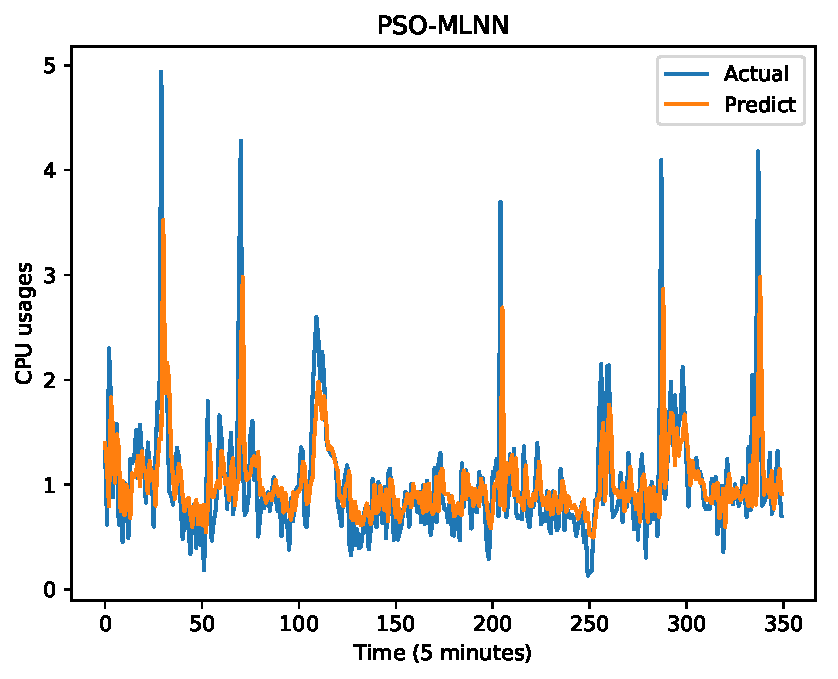
\includegraphics[width=0.9\linewidth]{images/pdf/predict/k2/cpu_k2_pso_mlnn.pdf} 
  \end{minipage}
  \begin{minipage}[b]{0.33\linewidth}
    \centering
    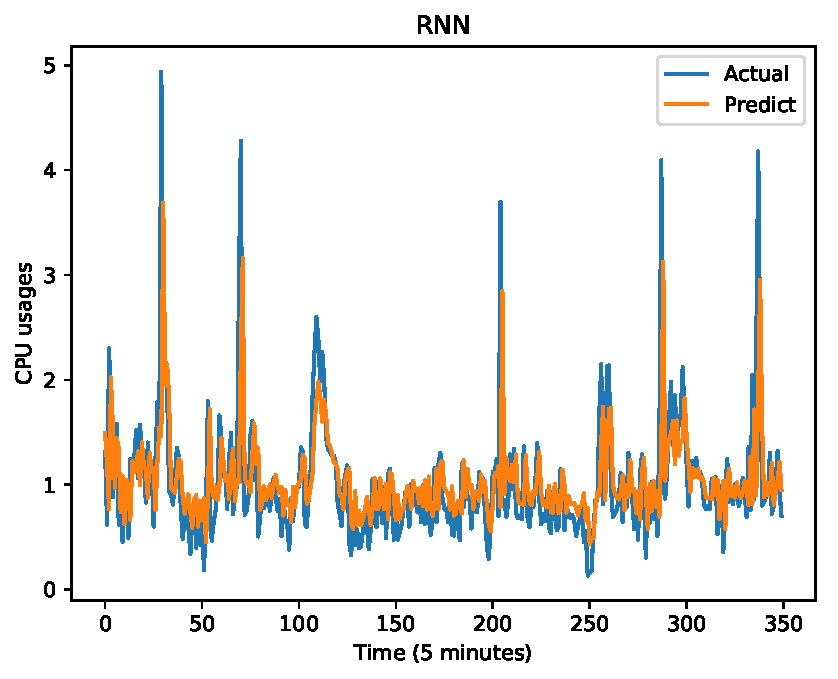
\includegraphics[width=0.9\linewidth]{images/pdf/predict/k2/cpu_k2_rnn.pdf} 
  \end{minipage} 
  \begin{minipage}[b]{0.33\linewidth}
    \centering
    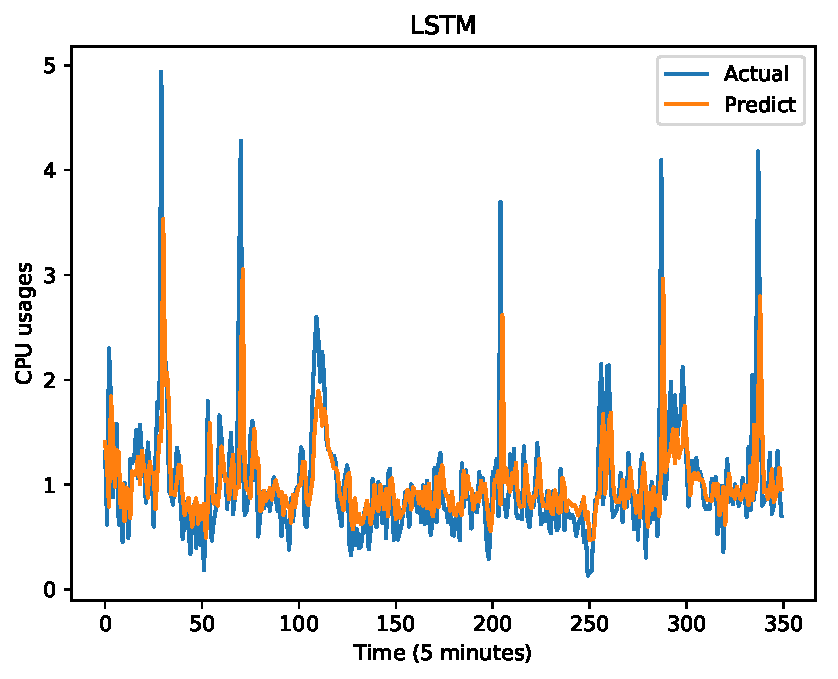
\includegraphics[width=0.9\linewidth]{images/pdf/predict/k2/cpu_k2_lstm.pdf} 
  \end{minipage} 
  
    \begin{minipage}[b]{0.33\linewidth}
    \centering
    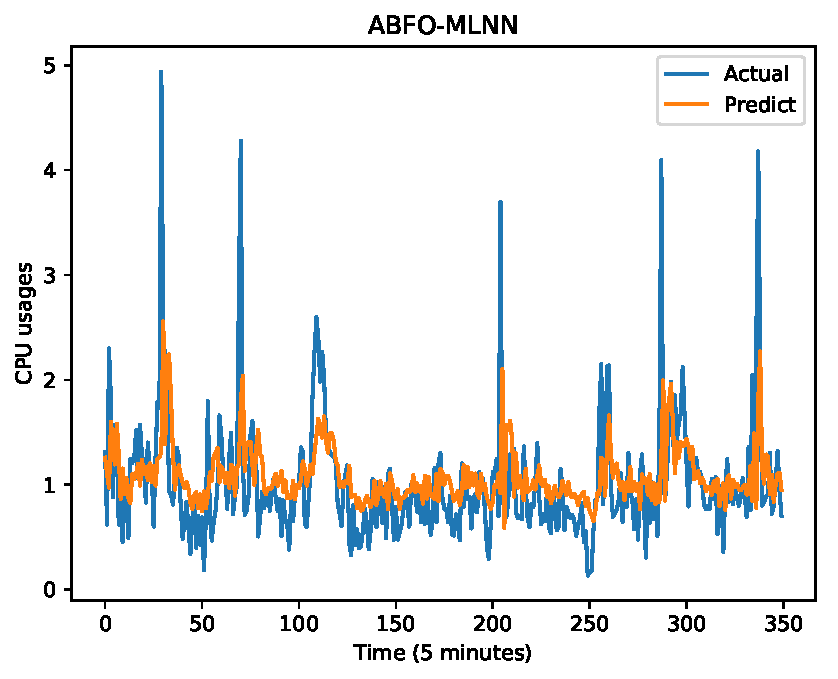
\includegraphics[width=0.9\linewidth]{images/pdf/predict/k2/cpu_k2_abfo_mlnn.pdf} 
  \end{minipage}
  \begin{minipage}[b]{0.33\linewidth}
    \centering
    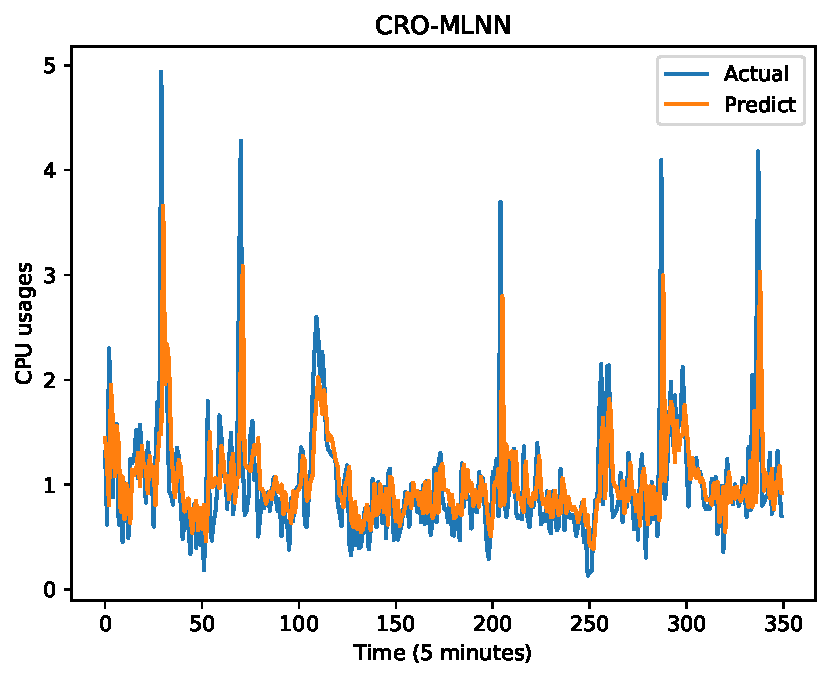
\includegraphics[width=0.9\linewidth]{images/pdf/predict/k2/cpu_k2_cro_mlnn.pdf} 
  \end{minipage} 
  \begin{minipage}[b]{0.33\linewidth}
    \centering
    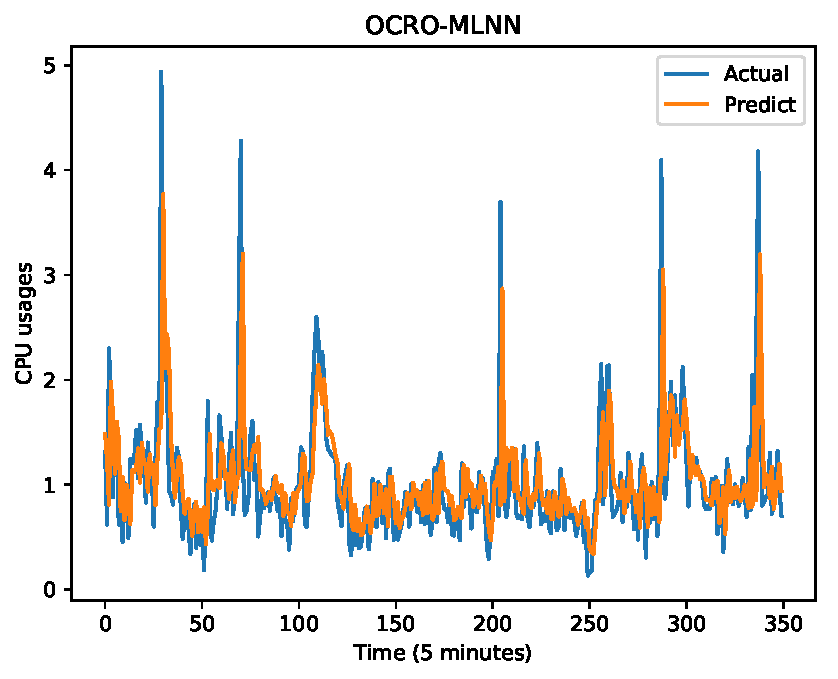
\includegraphics[width=0.9\linewidth]{images/pdf/predict/k2/cpu_k2_ocro_mlnn.pdf} 
  \end{minipage} 
  
  \caption{Comparison of OCRO-MLNN prediction with other models (sliding window $k$ = 2; multivariate data (CPU)} 
  \label{predict_cpu_sliding2} 
\end{figure}

\begin{figure}[!ht] 
  \begin{minipage}[b]{0.33\linewidth}
    \centering
    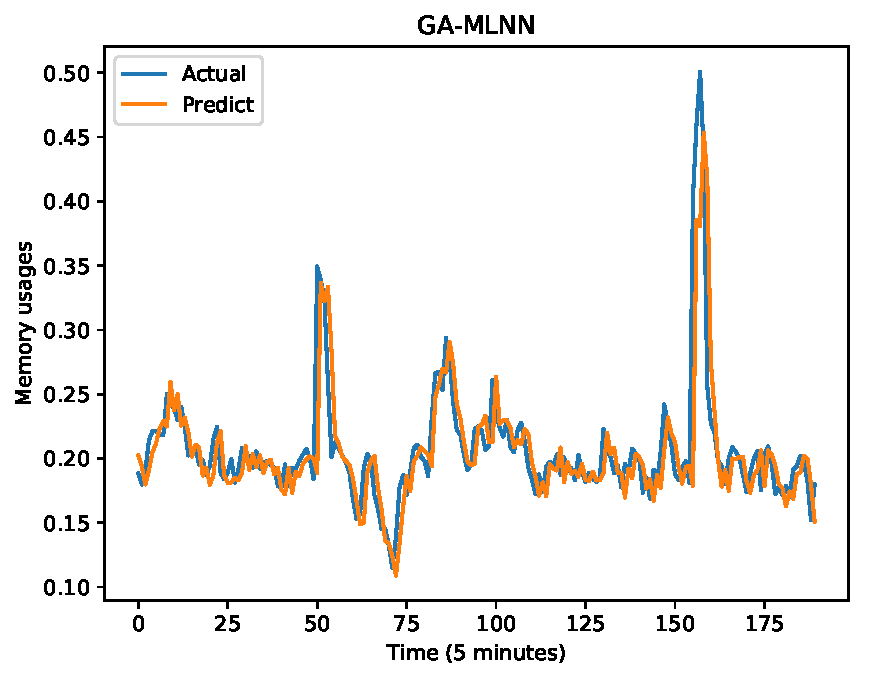
\includegraphics[width=0.9\linewidth]{images/pdf/predict/k5/ram_k5_ga_mlnn.pdf} 
  \end{minipage}
  \begin{minipage}[b]{0.33\linewidth}
    \centering
    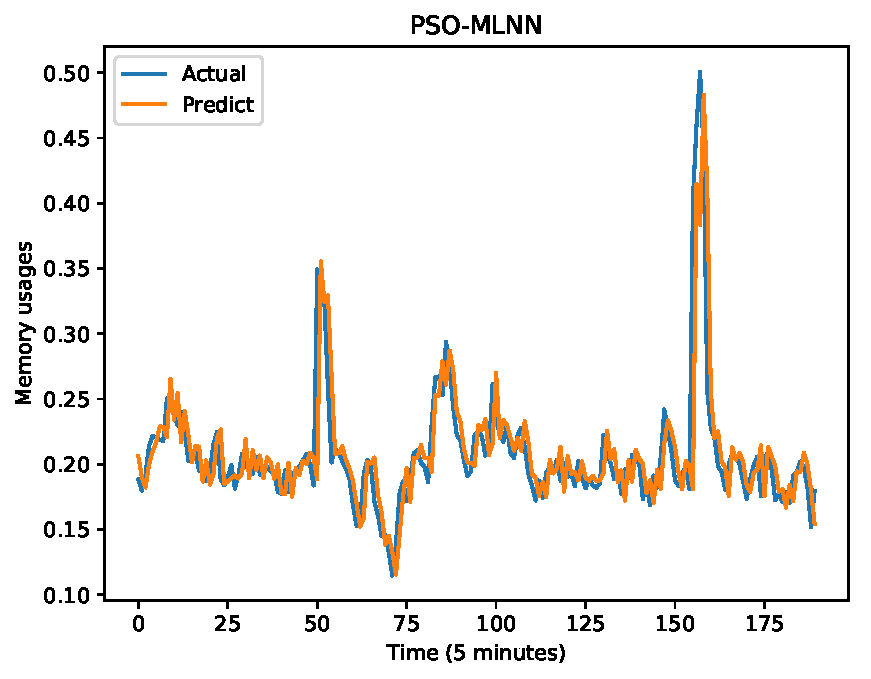
\includegraphics[width=0.9\linewidth]{images/pdf/predict/k5/ram_k5_pso_mlnn.pdf} 
  \end{minipage} 
  \begin{minipage}[b]{0.33\linewidth}
    \centering
    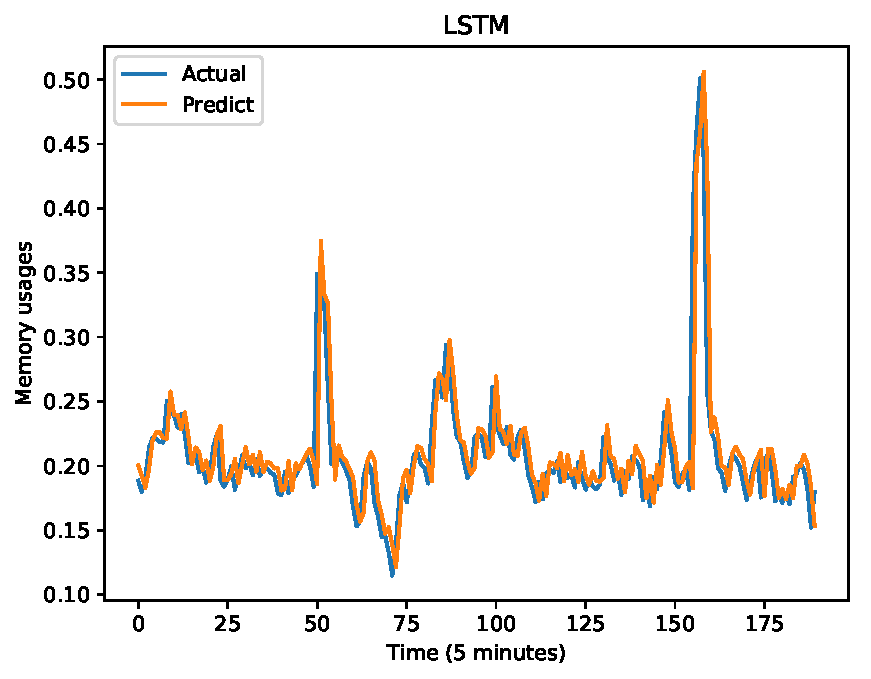
\includegraphics[width=0.9\linewidth]{images/pdf/predict/k5/ram_k5_lstm.pdf} 
  \end{minipage} 
  
    \begin{minipage}[b]{0.33\linewidth}
    \centering
    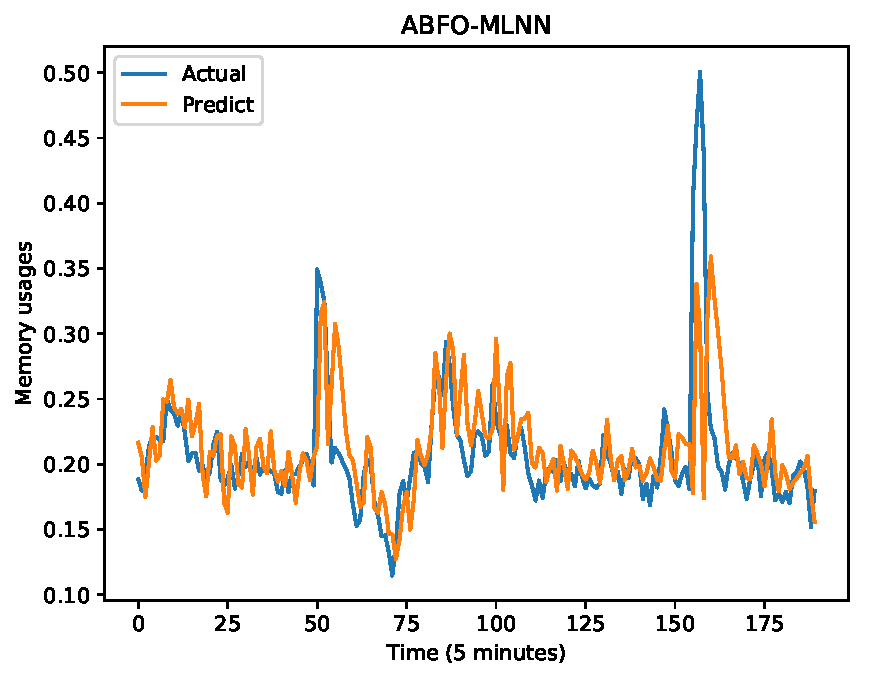
\includegraphics[width=0.9\linewidth]{images/pdf/predict/k5/ram_k5_abfo_mlnn.pdf} 
  \end{minipage}
  \begin{minipage}[b]{0.33\linewidth}
    \centering
    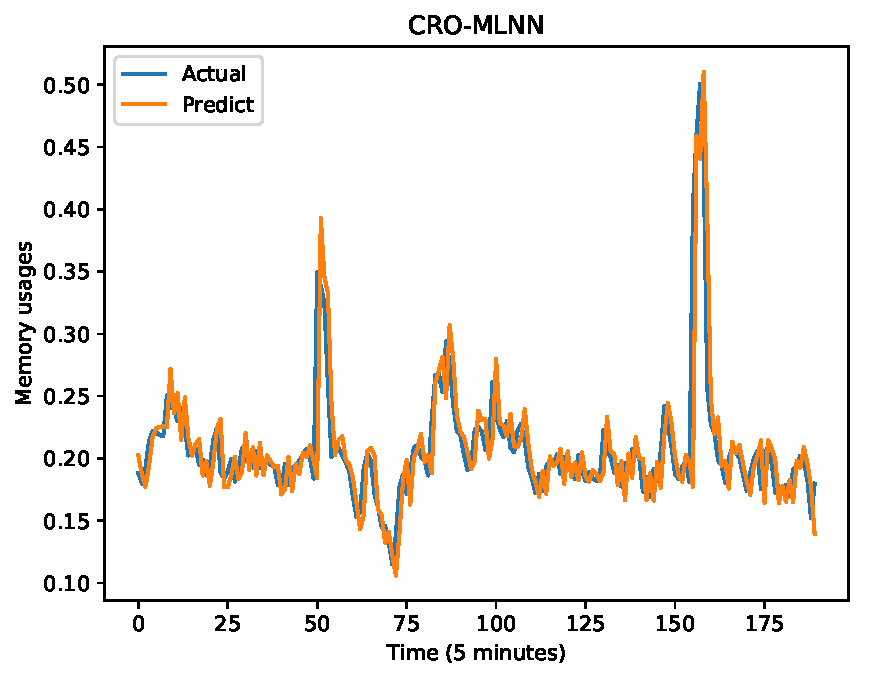
\includegraphics[width=0.9\linewidth]{images/pdf/predict/k5/ram_k5_cro_mlnn.pdf} 
  \end{minipage} 
  \begin{minipage}[b]{0.33\linewidth}
    \centering
    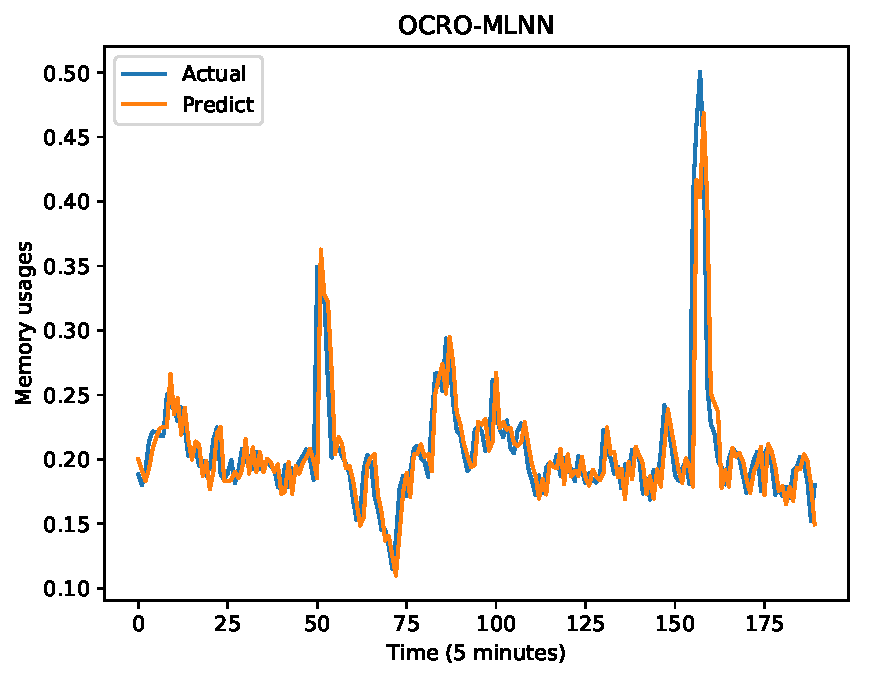
\includegraphics[width=0.9\linewidth]{images/pdf/predict/k5/ram_k5_ocro_mlnn.pdf} 
  \end{minipage} 
  
  \caption{Comparison of OCRO-MLNN prediction with other models (sliding window $k$ = 5; multivariate data (RAM)} 
  \label{predict_ram_sliding5} 
\end{figure}

\paragraph{\textbf{Runtime comparison.}} Table~\ref{table:multi_speed} presents outcomes of runtime experiments with different models. It can be seen that the obtained results of CRO-MLNN and OCRO-MLNN, which outperform other models on system runtime similarly as with univariate datasets. Concretely, for CPU metric with $k = 5$: CRO-MLNN and OCRO-MLNN runtime are 252.78s and 240.21s respectively. LSTM consumes approximately 5 times more (i.e. 1324.65s) to complete all training cycles. The difference is significant when the time series dataset for prediction is large-scale. Fig.~\ref{fig:speed_system_multivariate} visualizes system time of our OCRO-MLNN model (green color) in comparison with the rest.

%From the results and illustration in the table~\ref{table:multi_speed}, it's obsereved that CRO-MLNN and OCRO-MLNN once again outperform other models in consuming least time for system as it is in univariate-datasets. Let's look at CPU metric's results with $k = 5$, while CRO-MLNN and OCRO-MLNN need only about 252.78s and 240.21s respectively, LSTM consumes approxiately 5 times CRO-MLNN and OCRO-MLNN which is 1324.65s to complete all training system. This difference is really significant when apply those models into reality time series prediction problems. Fig.~\ref{fig:speed_system_multivariate} visualize system time of our OCRO-MLNN model (green color) and other models.

\begin{figure}
	\centering
	\begin{minipage}[t]{1.0\textwidth}
		\centering
		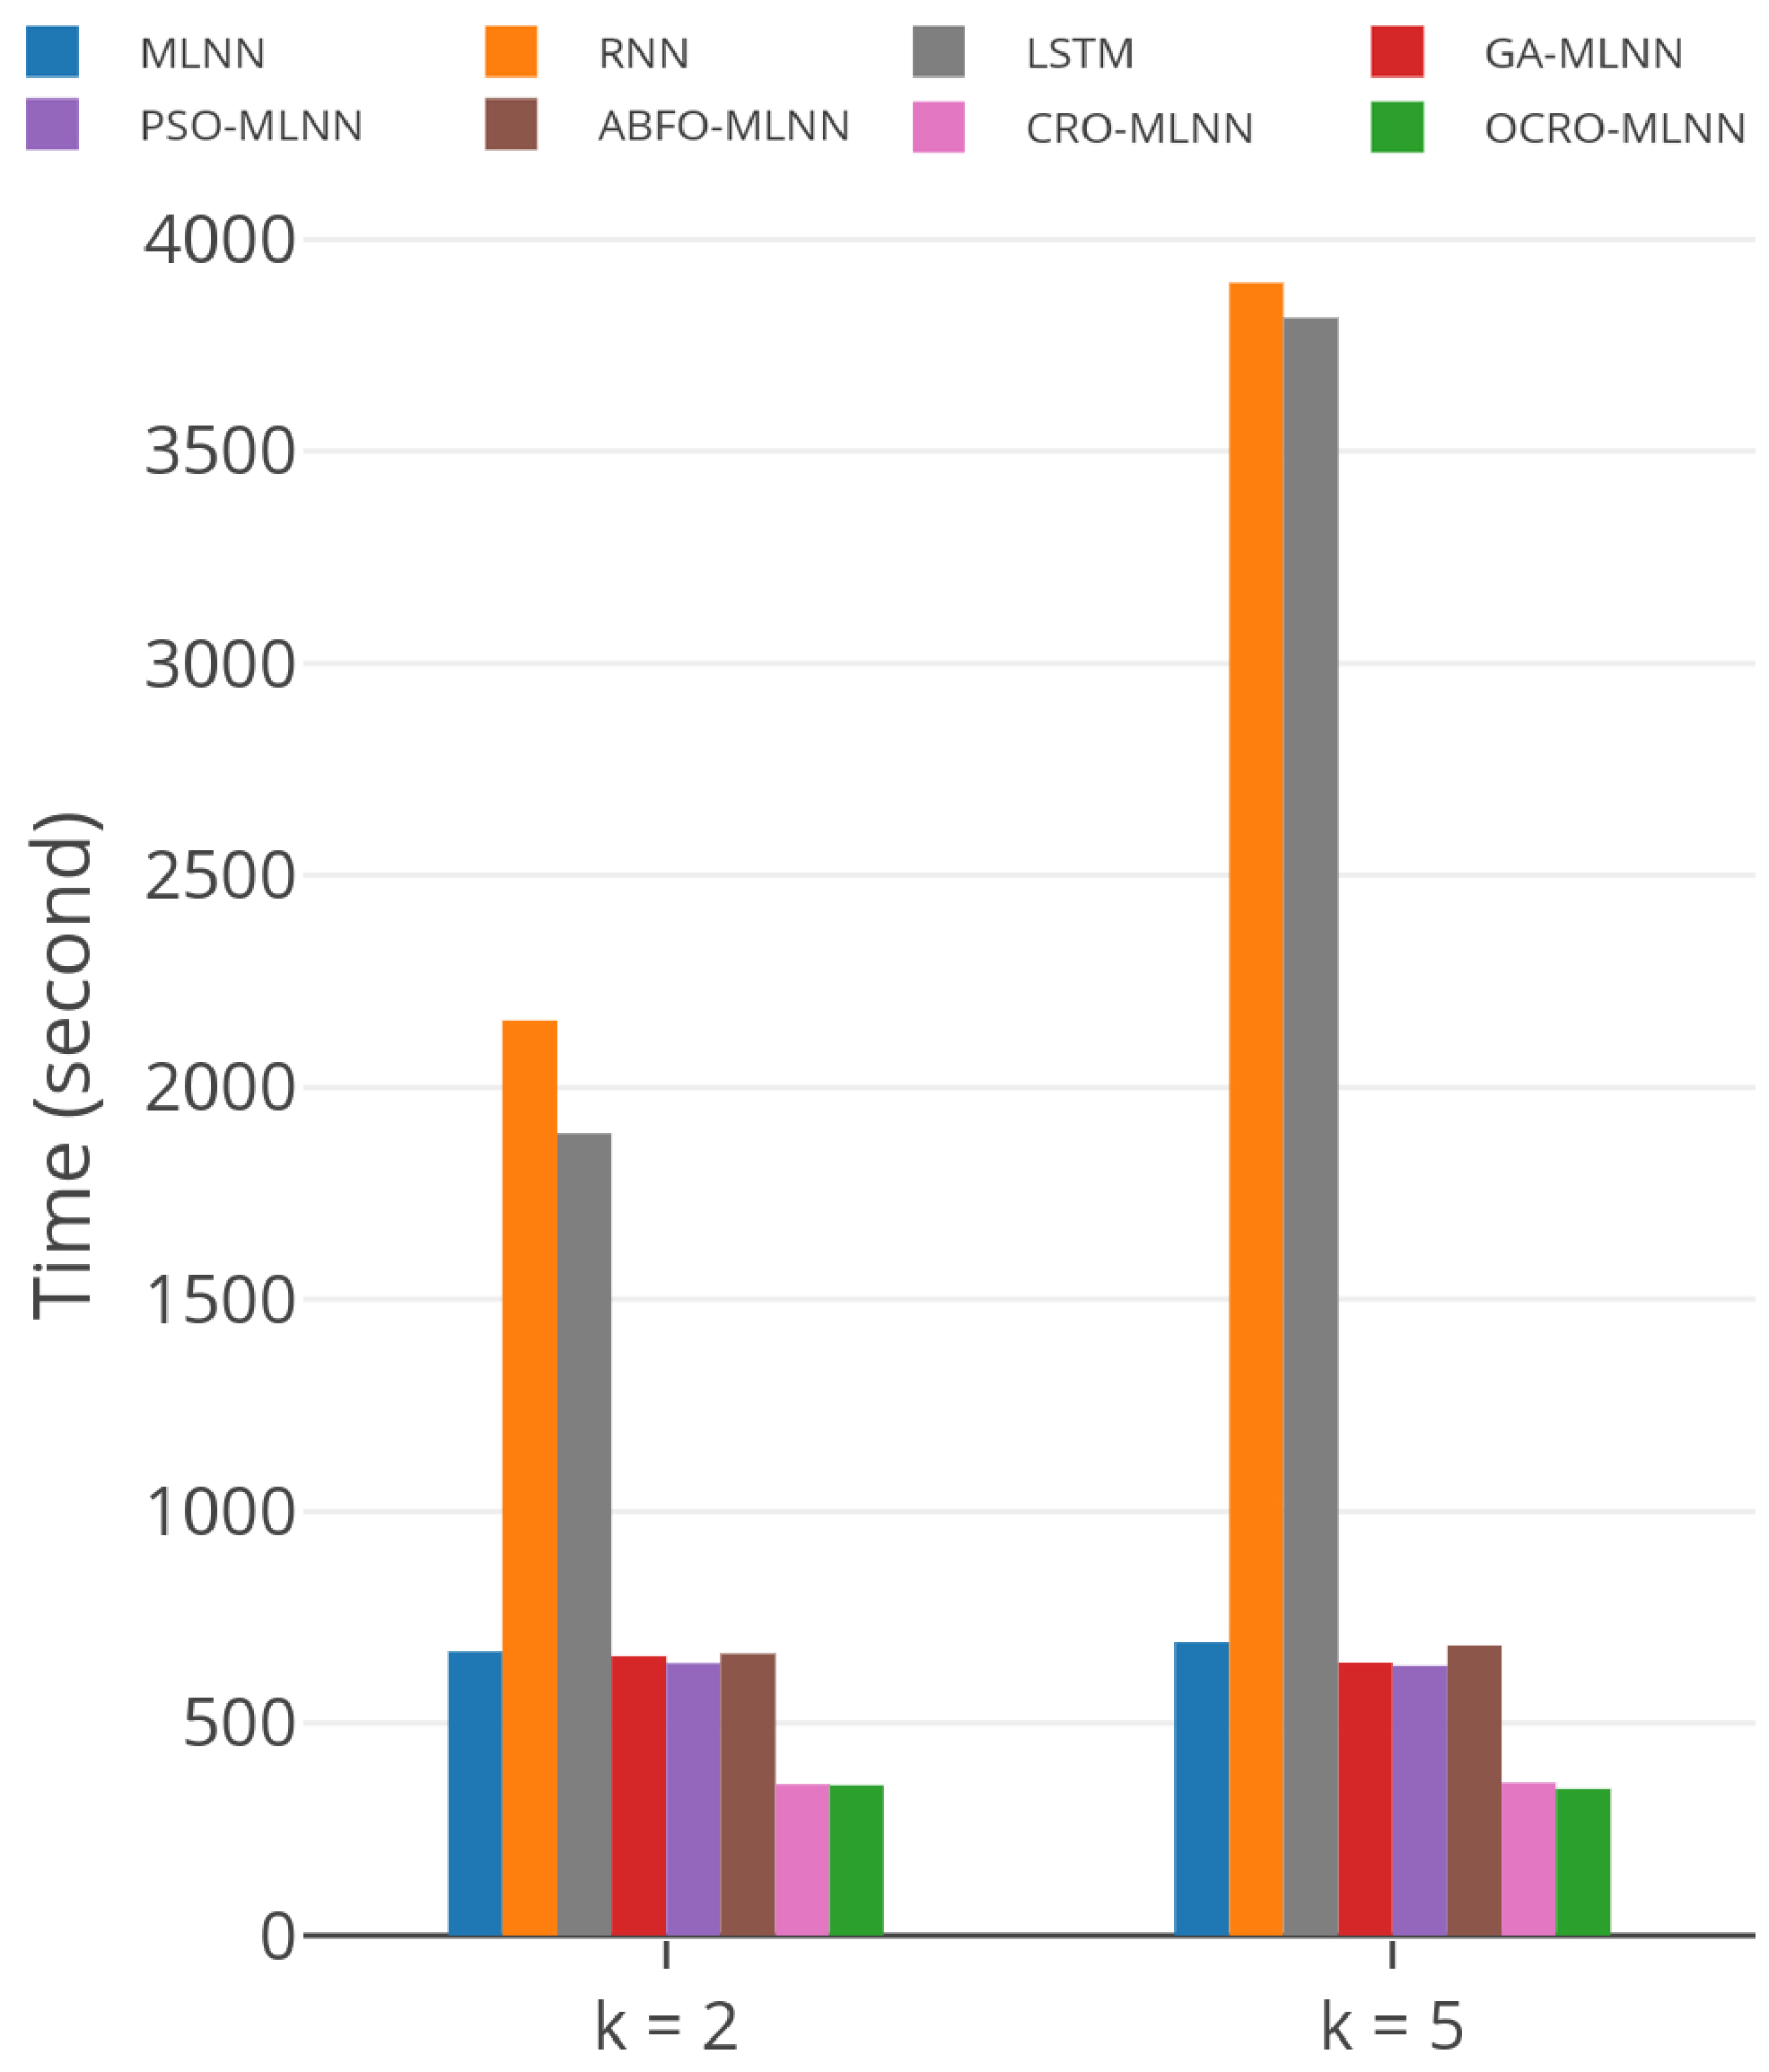
\includegraphics[width=0.45\textwidth =0cm 0cm 0cm 0cm, height = 8cm]{images/pdf/time/time_eu.pdf}
%	\end{minipage}
%	\begin{minipage}[t]{8cm}
		\centering
		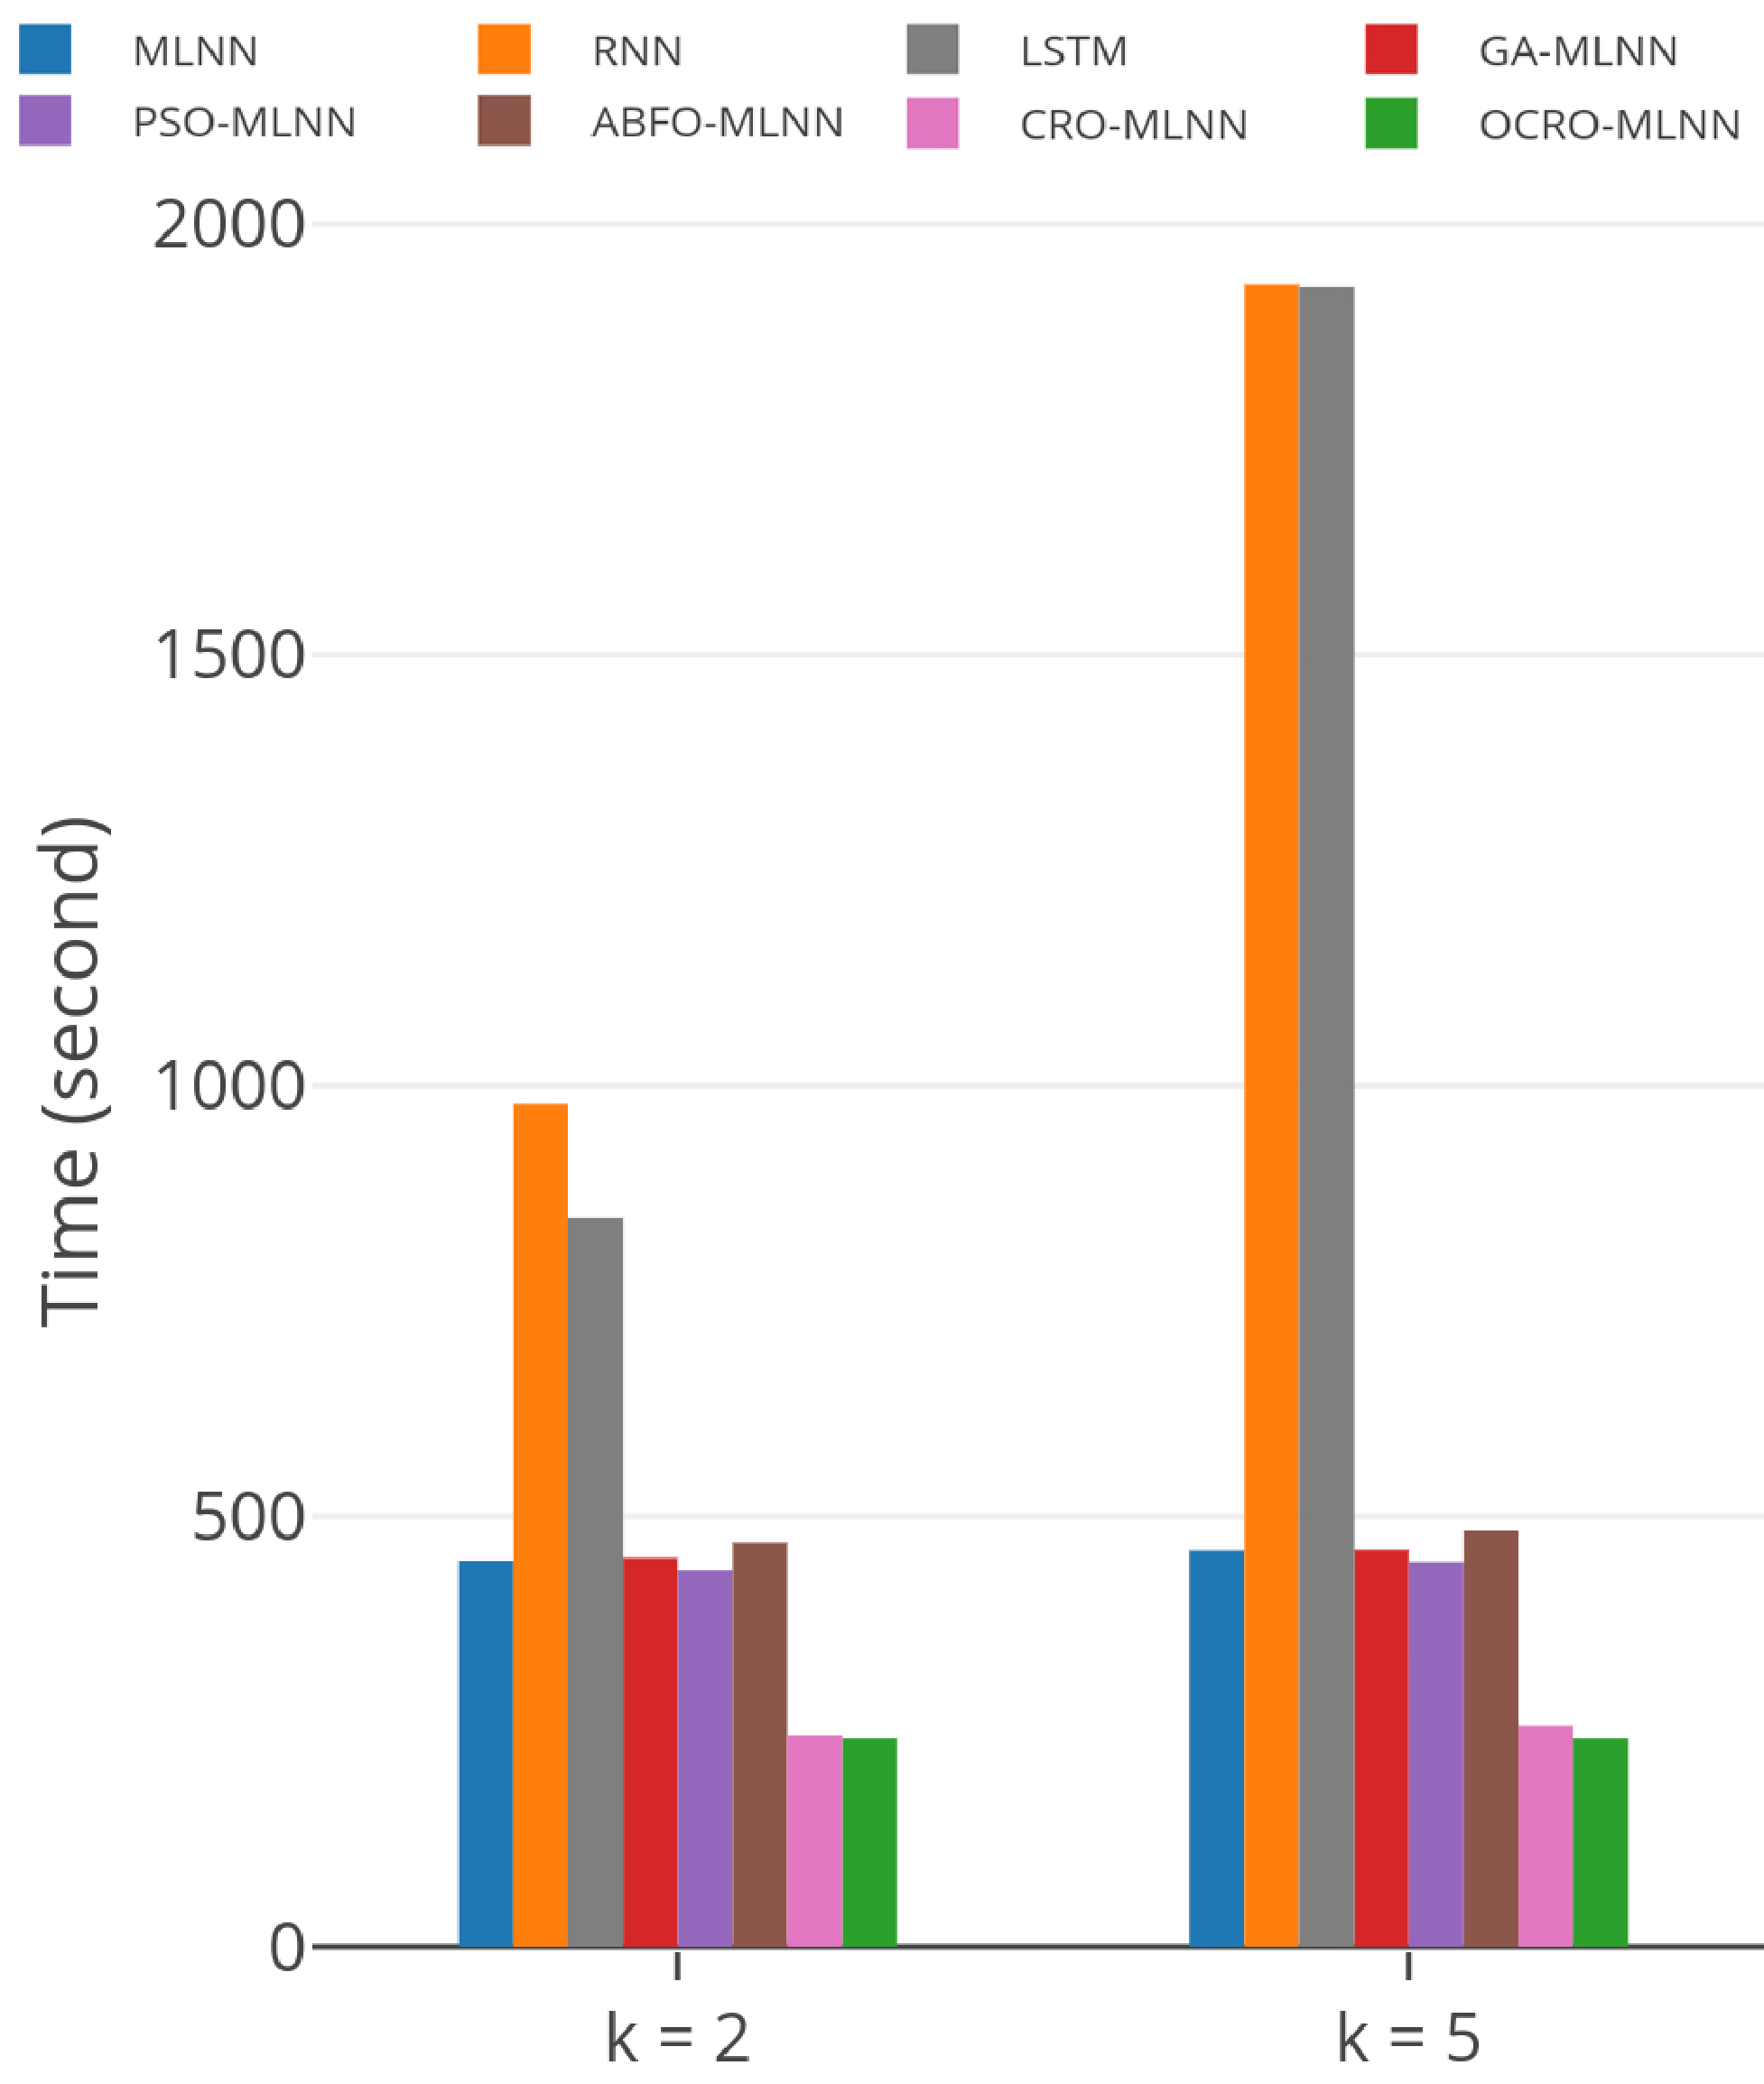
\includegraphics[width=0.45\textwidth =0cm 0cm 0cm 0cm, height = 8cm]{images/pdf/time/time_wc.pdf}
	\end{minipage}
	\caption{Runtime comparison: OCRO-MLNN (green), sliding window $k$ = 2 and $k$ = 5; univariate data: EU (left), WC (right)} 
	\label{fig:speed_system_univariate}
\end{figure}

\begin{figure}
	\centering
	\begin{minipage}[t]{1.0\textwidth}
		\centering
		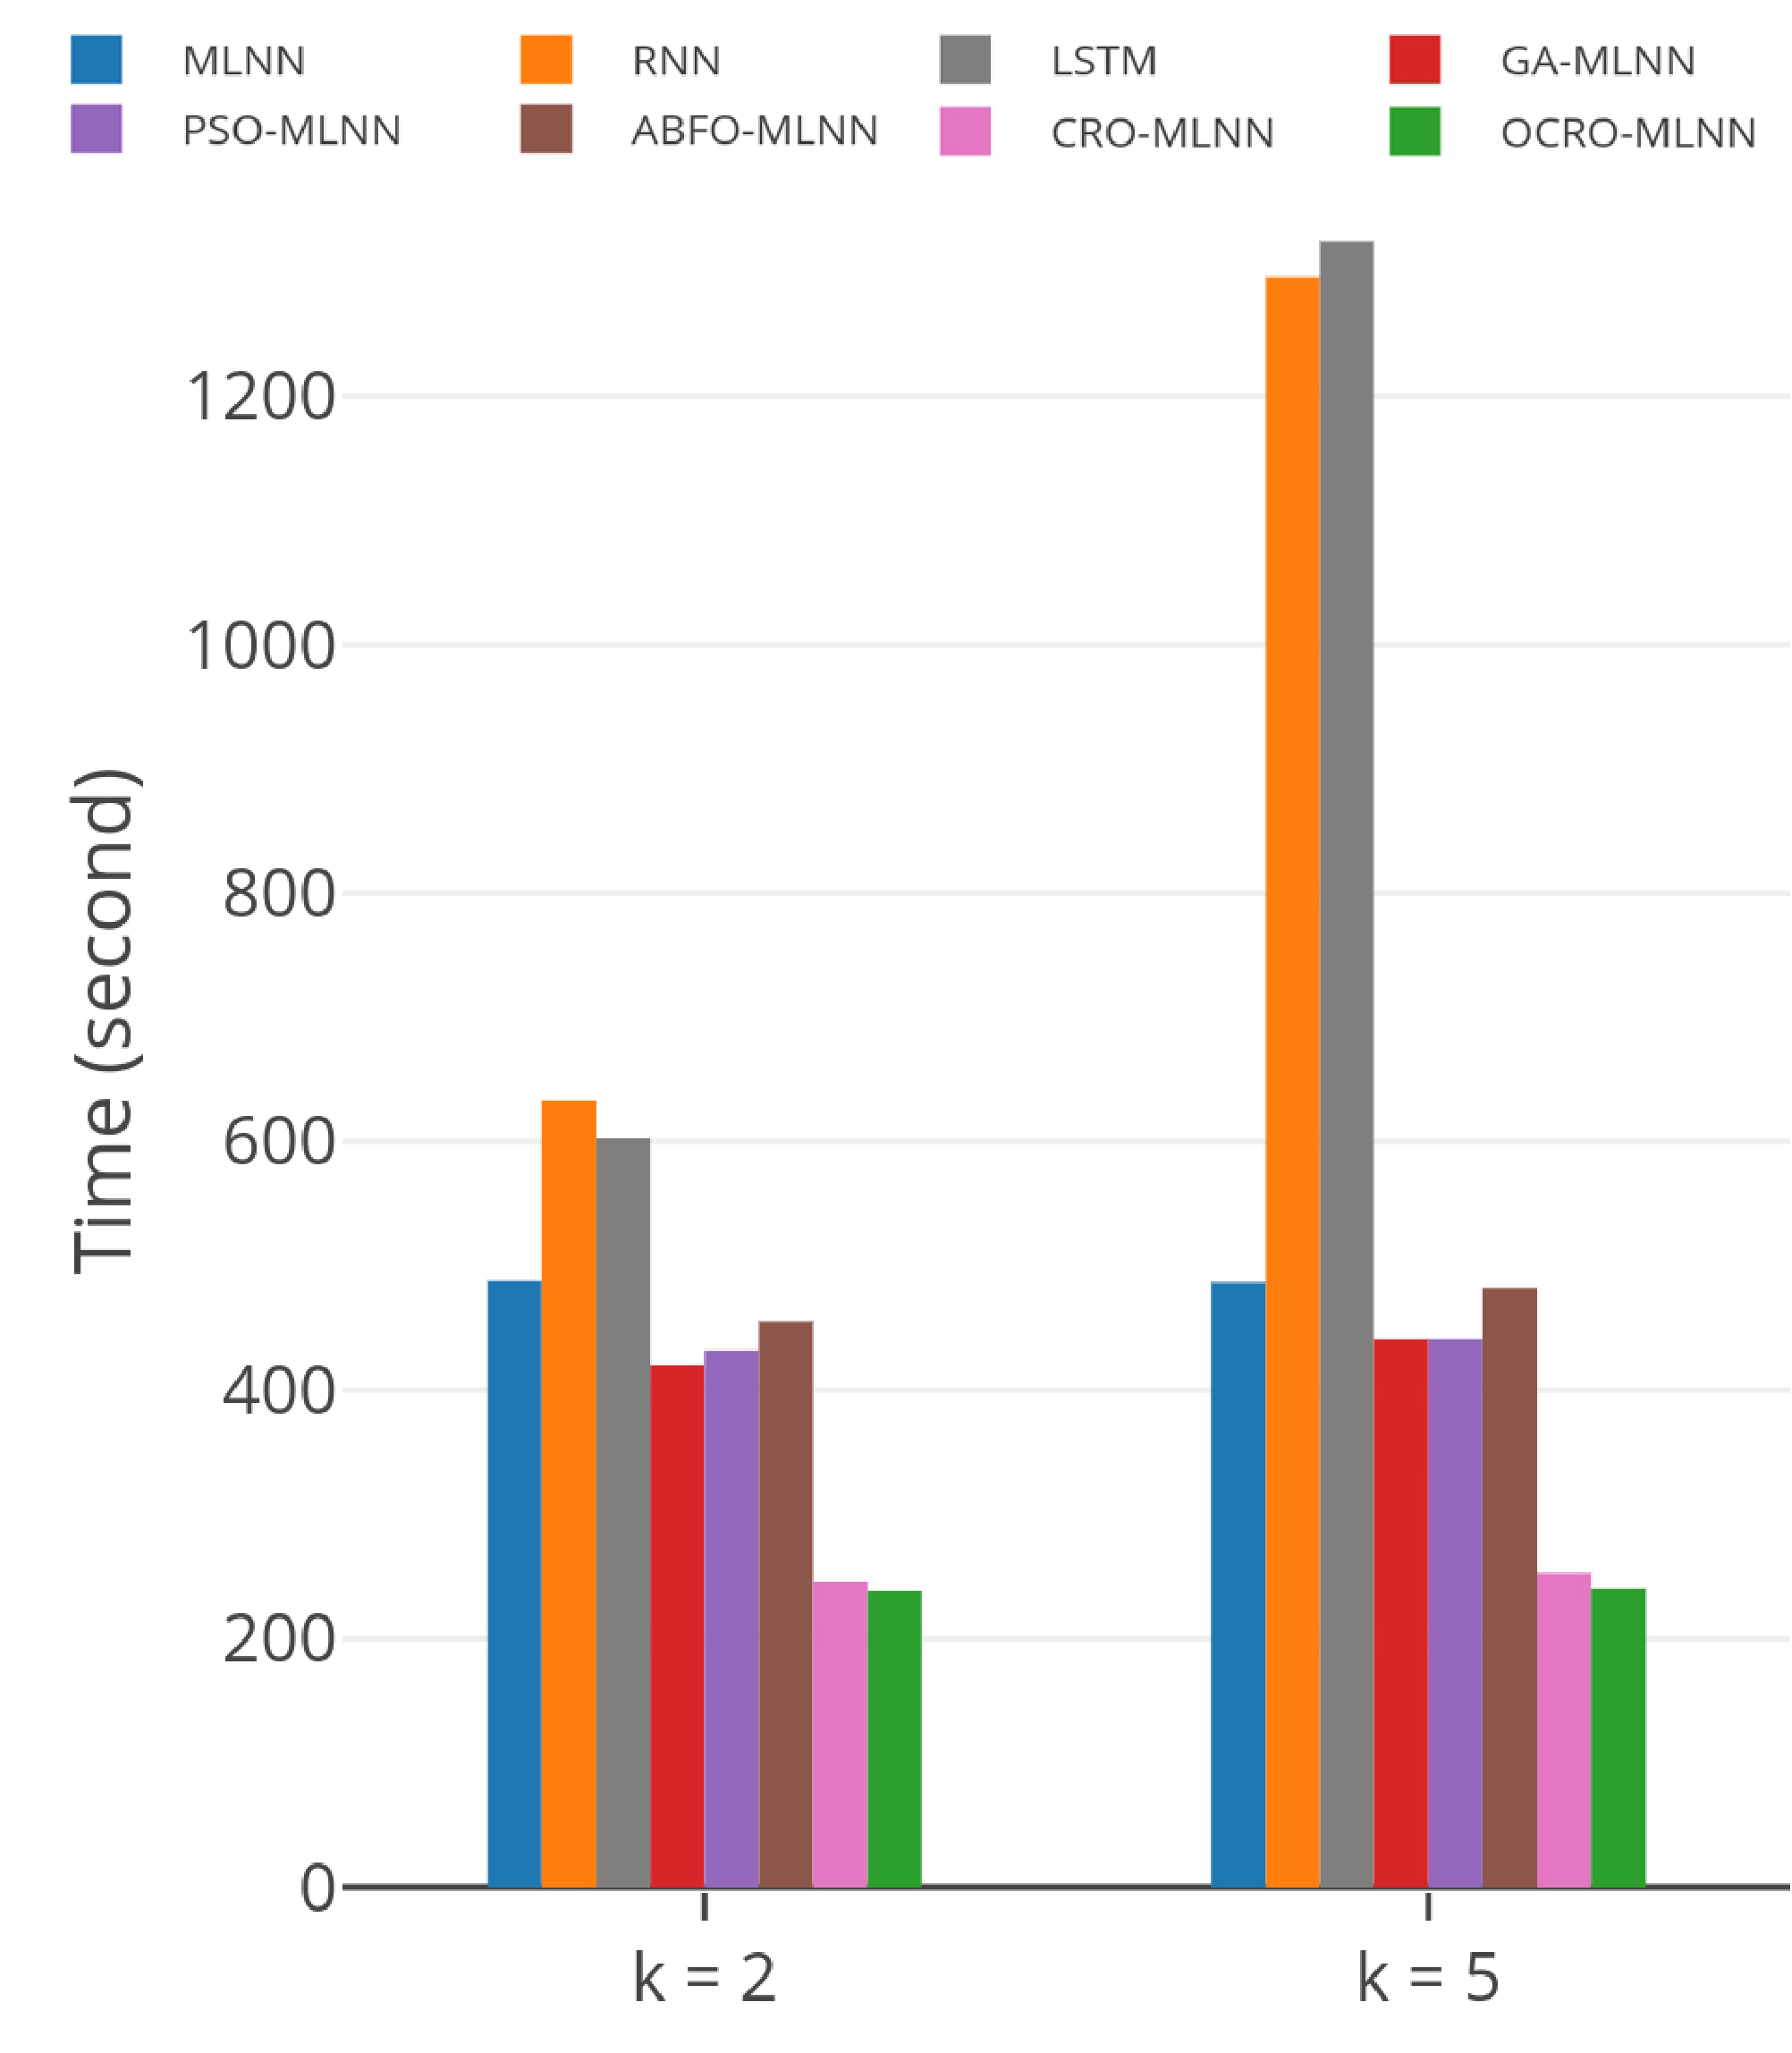
\includegraphics[width=0.45\textwidth =0cm 0cm 0cm 0cm, height = 8cm]{images/pdf/time/time_cpu.pdf}
%	\end{minipage}
%	\begin{minipage}[t]{8cm}
		\centering
		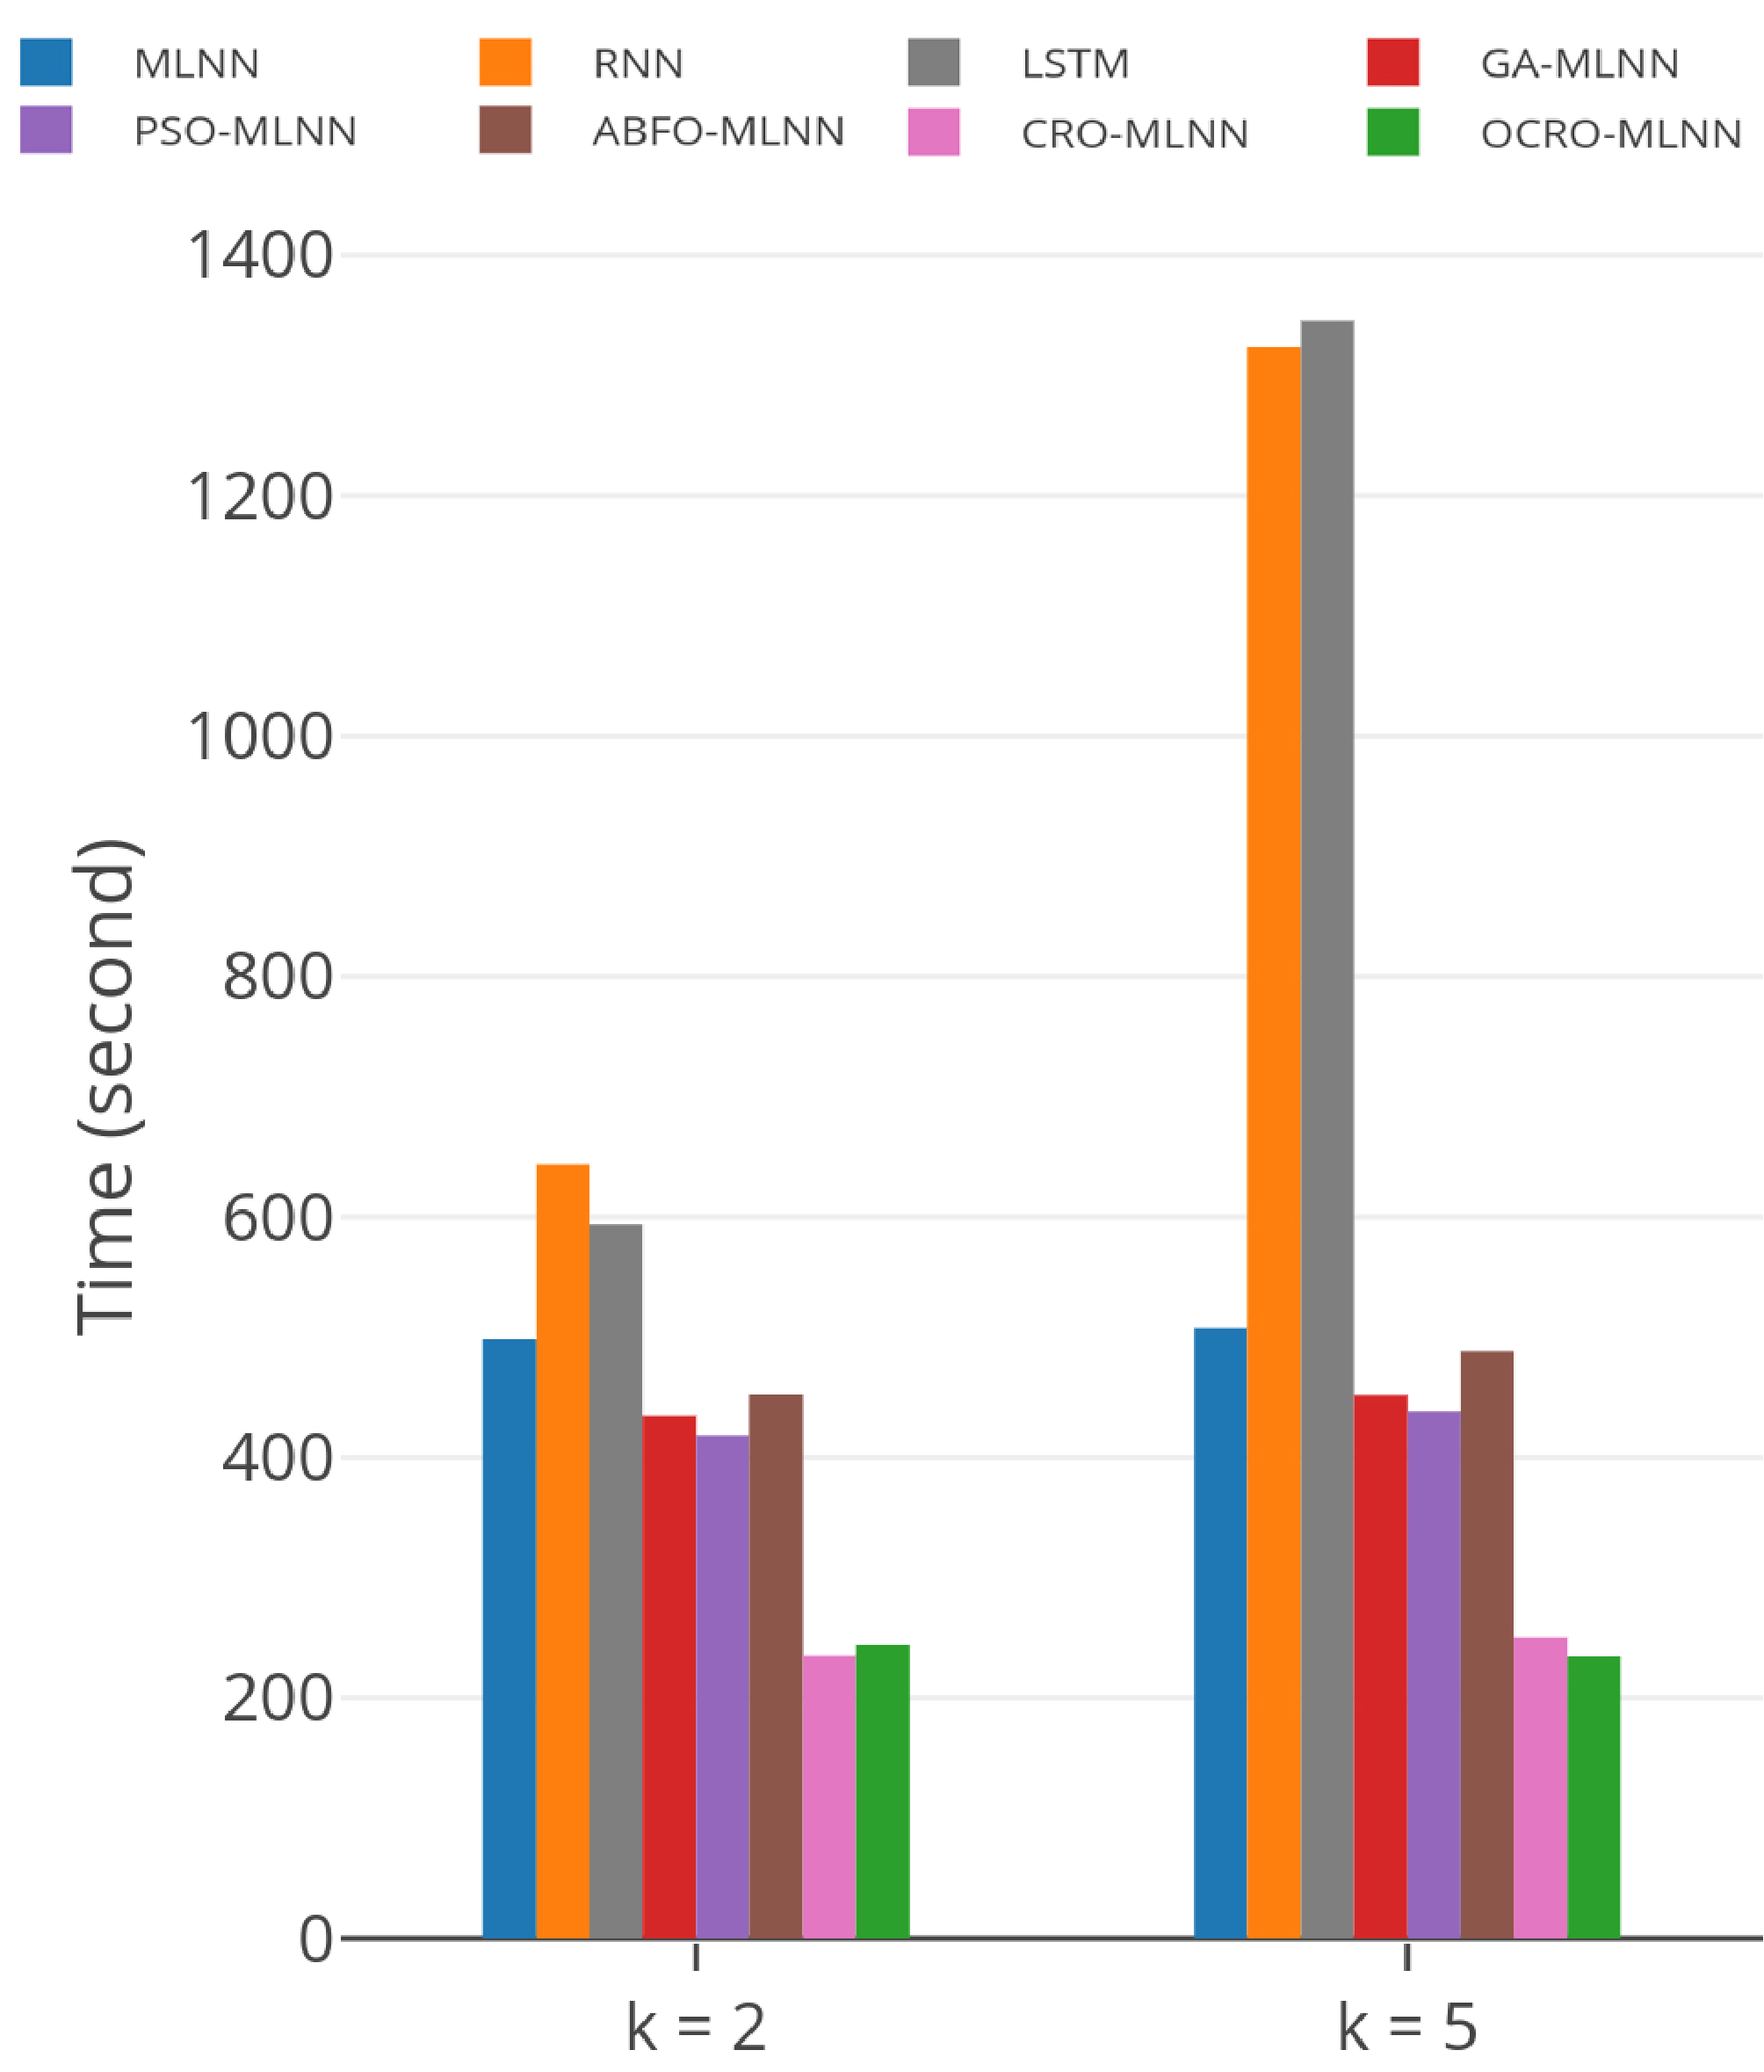
\includegraphics[width=0.45\textwidth =0cm 0cm 0cm 0cm, height = 8cm]{images/pdf/time/time_ram.pdf}
	\end{minipage}
	\caption{Runtime comparison: OCRO-MLNN (green), sliding window $k$ = 2 and $k$ = 5; multivariate data, CPU (left), RAM (right)} 
	\label{fig:speed_system_multivariate}
\end{figure}

% ======================= Table Multivariate Speed  ================================
% fit-width table
\begin{table}[!h]
	\caption{Runtime comparison (sliding window $k$ = 2 and $k$ = 5, multivariate dataset)}
	\label{table:multi_speed}
	\centering
	\begin{adjustbox}{width=0.7\textwidth}
%	\begin{sideways}
		\begin{tabular}{| c | c | c | c | c | c | c | c |}%
			\hline
			\multirow{2}{*}{Data} & \multirow{2}{*}{Model} & \multicolumn{3}{c|}{$k$ = 2} & \multicolumn{3}{c|}{ $k$ = 5 } \\ \cline{3-8}
   				& & $t_e$ & $t_p$ & $\boldsymbol{t_s}$ & $t_e$ & $t_p$ & $\boldsymbol{t_s}$  \\ [0.5ex] \hline
			\primitiveinput{table/table_multi_speed}
			\hline
		\end{tabular}
%	\end{sideways}
	\end{adjustbox}
\end{table}

\paragraph{\textbf{Model stability.}} Table~\ref{table:multi_stability} gives summary statistics of RMSE error with the tested models after 15 run times. The evaluations gained through these experiments with multivariate data include:
\begin{itemize}
	\item MLNN and RNN are quite unstable (as usually) due to back-propagation dependence on the initial weights. LSTM has smaller fluctuation of RMSE's error at the cost of its complex structure. Specifically, for CPU metrics, $k = 2$, standard deviation ($std$) of MLNN, RNN and LSTM model are $std = 0.0615$, 0.0353 and 0.0171, respectively. 
	\item The proposed approach to apply meta-heuristic OCRO to optimization problems gives more stability than gradient decent approach. The reason is that OCRO is considered as an efficient and powerful searching algorithm to help it jump out the local optimal and search for the best solution. So that when combining OCRO with traditional MLNN, the achieved model can work well under different conditions. 
	\item Compared to CPU metrics and $k = 5$, LSTM's $std = 0.0172$ and OCRO-MLNN's $std= 0.0058$ (i.e. one third of LSTM's $std$ value). Meanwhile, compared to RAM metrics, $k$ = 2, LSTM's $cv = 0.0293$ and OCRO-MLNN's $cv=0.0149$ (i.e. a half of LSTM's $cv$ value). 
\end{itemize}

Fig.~\ref{fig:stability_multi} expresses average RMSE after 15 run times of all models (the same way as univariate dataset).

% ============================ Table: Multivariate Stability =============================
% Fit-width table
\begin{table}[h]
	\caption{RMSE compparison (average of 15 times; multivariate dataset)}
	\label{table:multi_stability}
	\centering
	\begin{adjustbox}{width=\textwidth}
%	\begin{sideways}
		\begin{tabular}{| c | c| c | c | c | c | c | c | c | c | c | c |}%
		\hline
			 \multirow{2}{*}{Data} & \multirow{2}{*}{Model} & \multicolumn{5}{c|}{$k$ = 2} & \multicolumn{5}{c|}{ $k$ = 5 } \\ 
			 \cline{3-12}
	   		& & $min$ & $max$ & $mean$ & $std$ & $cv$ &   $min$ & $max$ & $mean$ & $std$ & $cv$ \\ [0.5ex] 
		\hline
			\primitiveinput{table/table_multi_stability}
		\hline
		\end{tabular}
%	\end{sideways}
	\end{adjustbox}
\end{table}

%% Rotated and fit-heigh table 
%\begin{table}
%	\caption{Summary statistics in error RMSE of our proposed OCRO-MLNN and other models after 15 run times (univariate dataset)}
%	\label{table:multi_speed_rotate}
%	\centering
%	\begin{adjustbox}{height=\textheight}
%	\begin{sideways}
%		\begin{tabular}{| c | c| c | c | c | c | c | c | c | c | c | c |}%
%			\hline
%			 \multirow{2}{*}{Data} & \multirow{2}{*}{Model} & \multicolumn{5}{c|}{k = 2} & \multicolumn{5}{c|}{ k = 5 } \\ \cline{3-12}
%	   		& & $min$ & $max$ & $mean$ & $std$ & $cv$ &   $min$ & $max$ & $mean$ & $std$ & $cv$ \\ [0.5ex] 
%			\hline
%			\primitiveinput{table/table_multi_stability}
%			\hline
%		\end{tabular}
%	\end{sideways}
%	\end{adjustbox}
%\end{table}

\begin{figure}
	\centering
	\begin{minipage}[t]{1\textwidth}
		\centering
		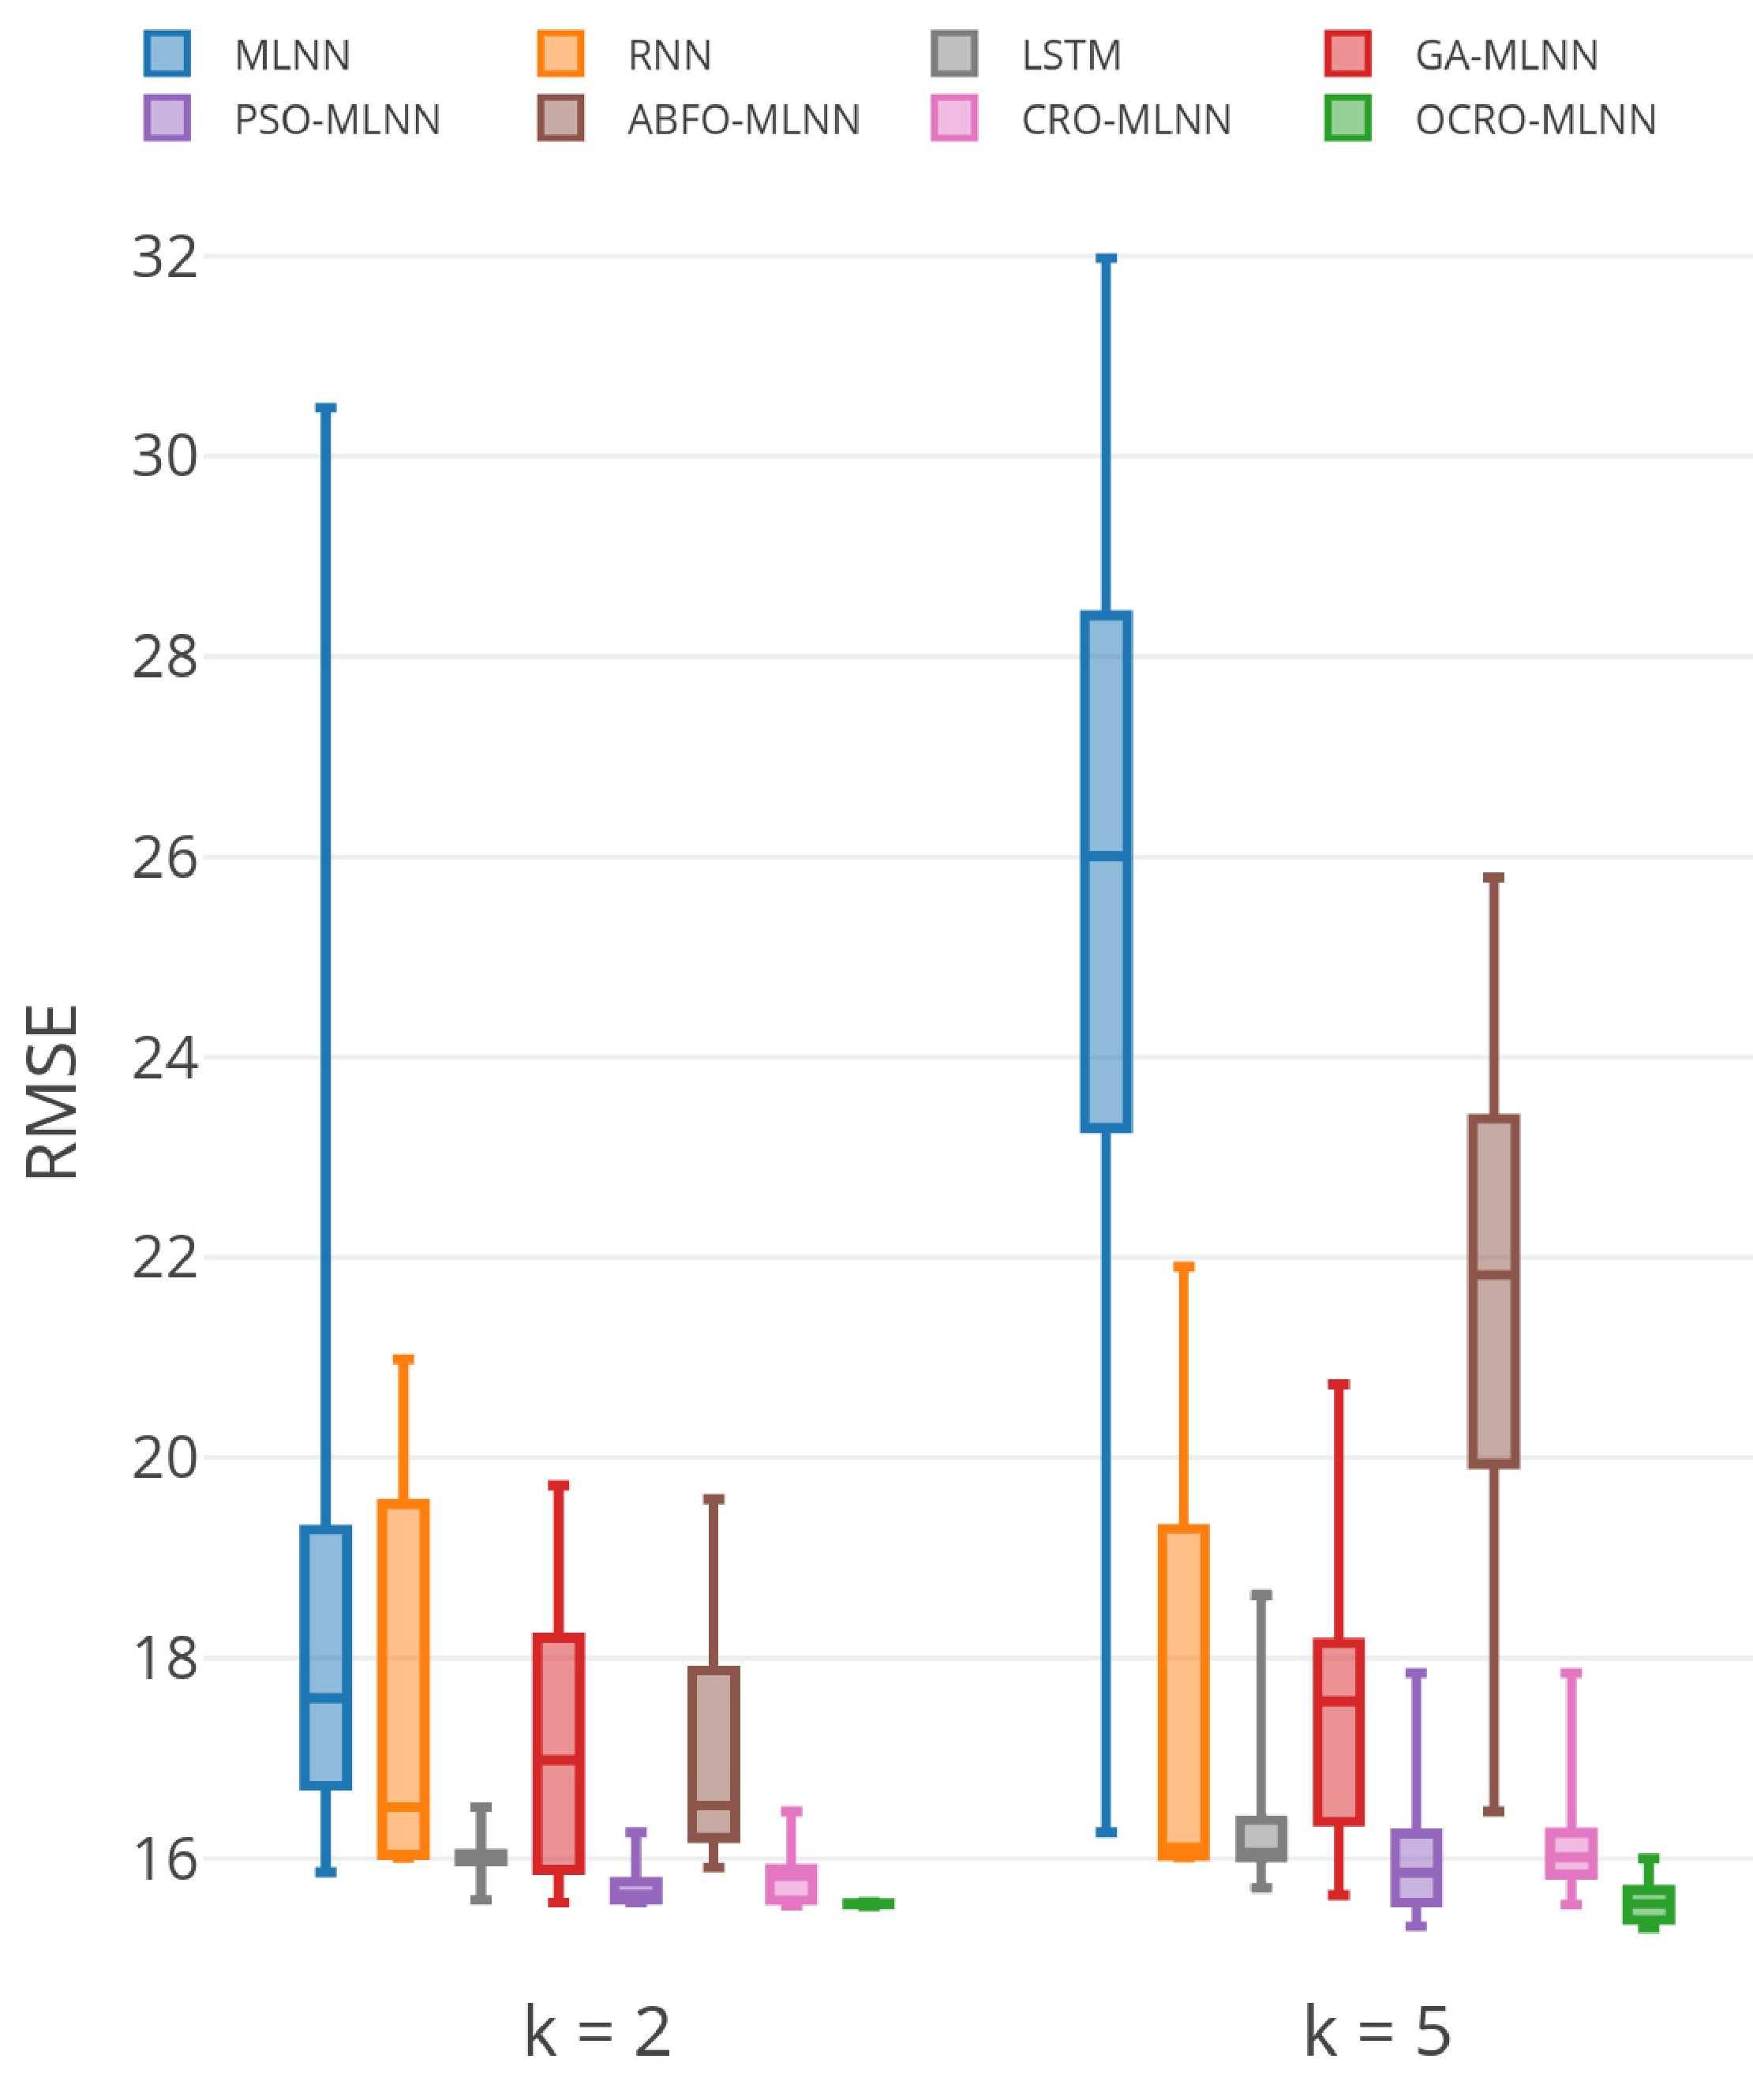
\includegraphics[width=0.45\textwidth =0cm 0cm 0cm 0cm, height = 8cm]{images/pdf/stability/st_eu_2.pdf}
%	\end{minipage}
%	\begin{minipage}[t]{8cm}
		\centering
		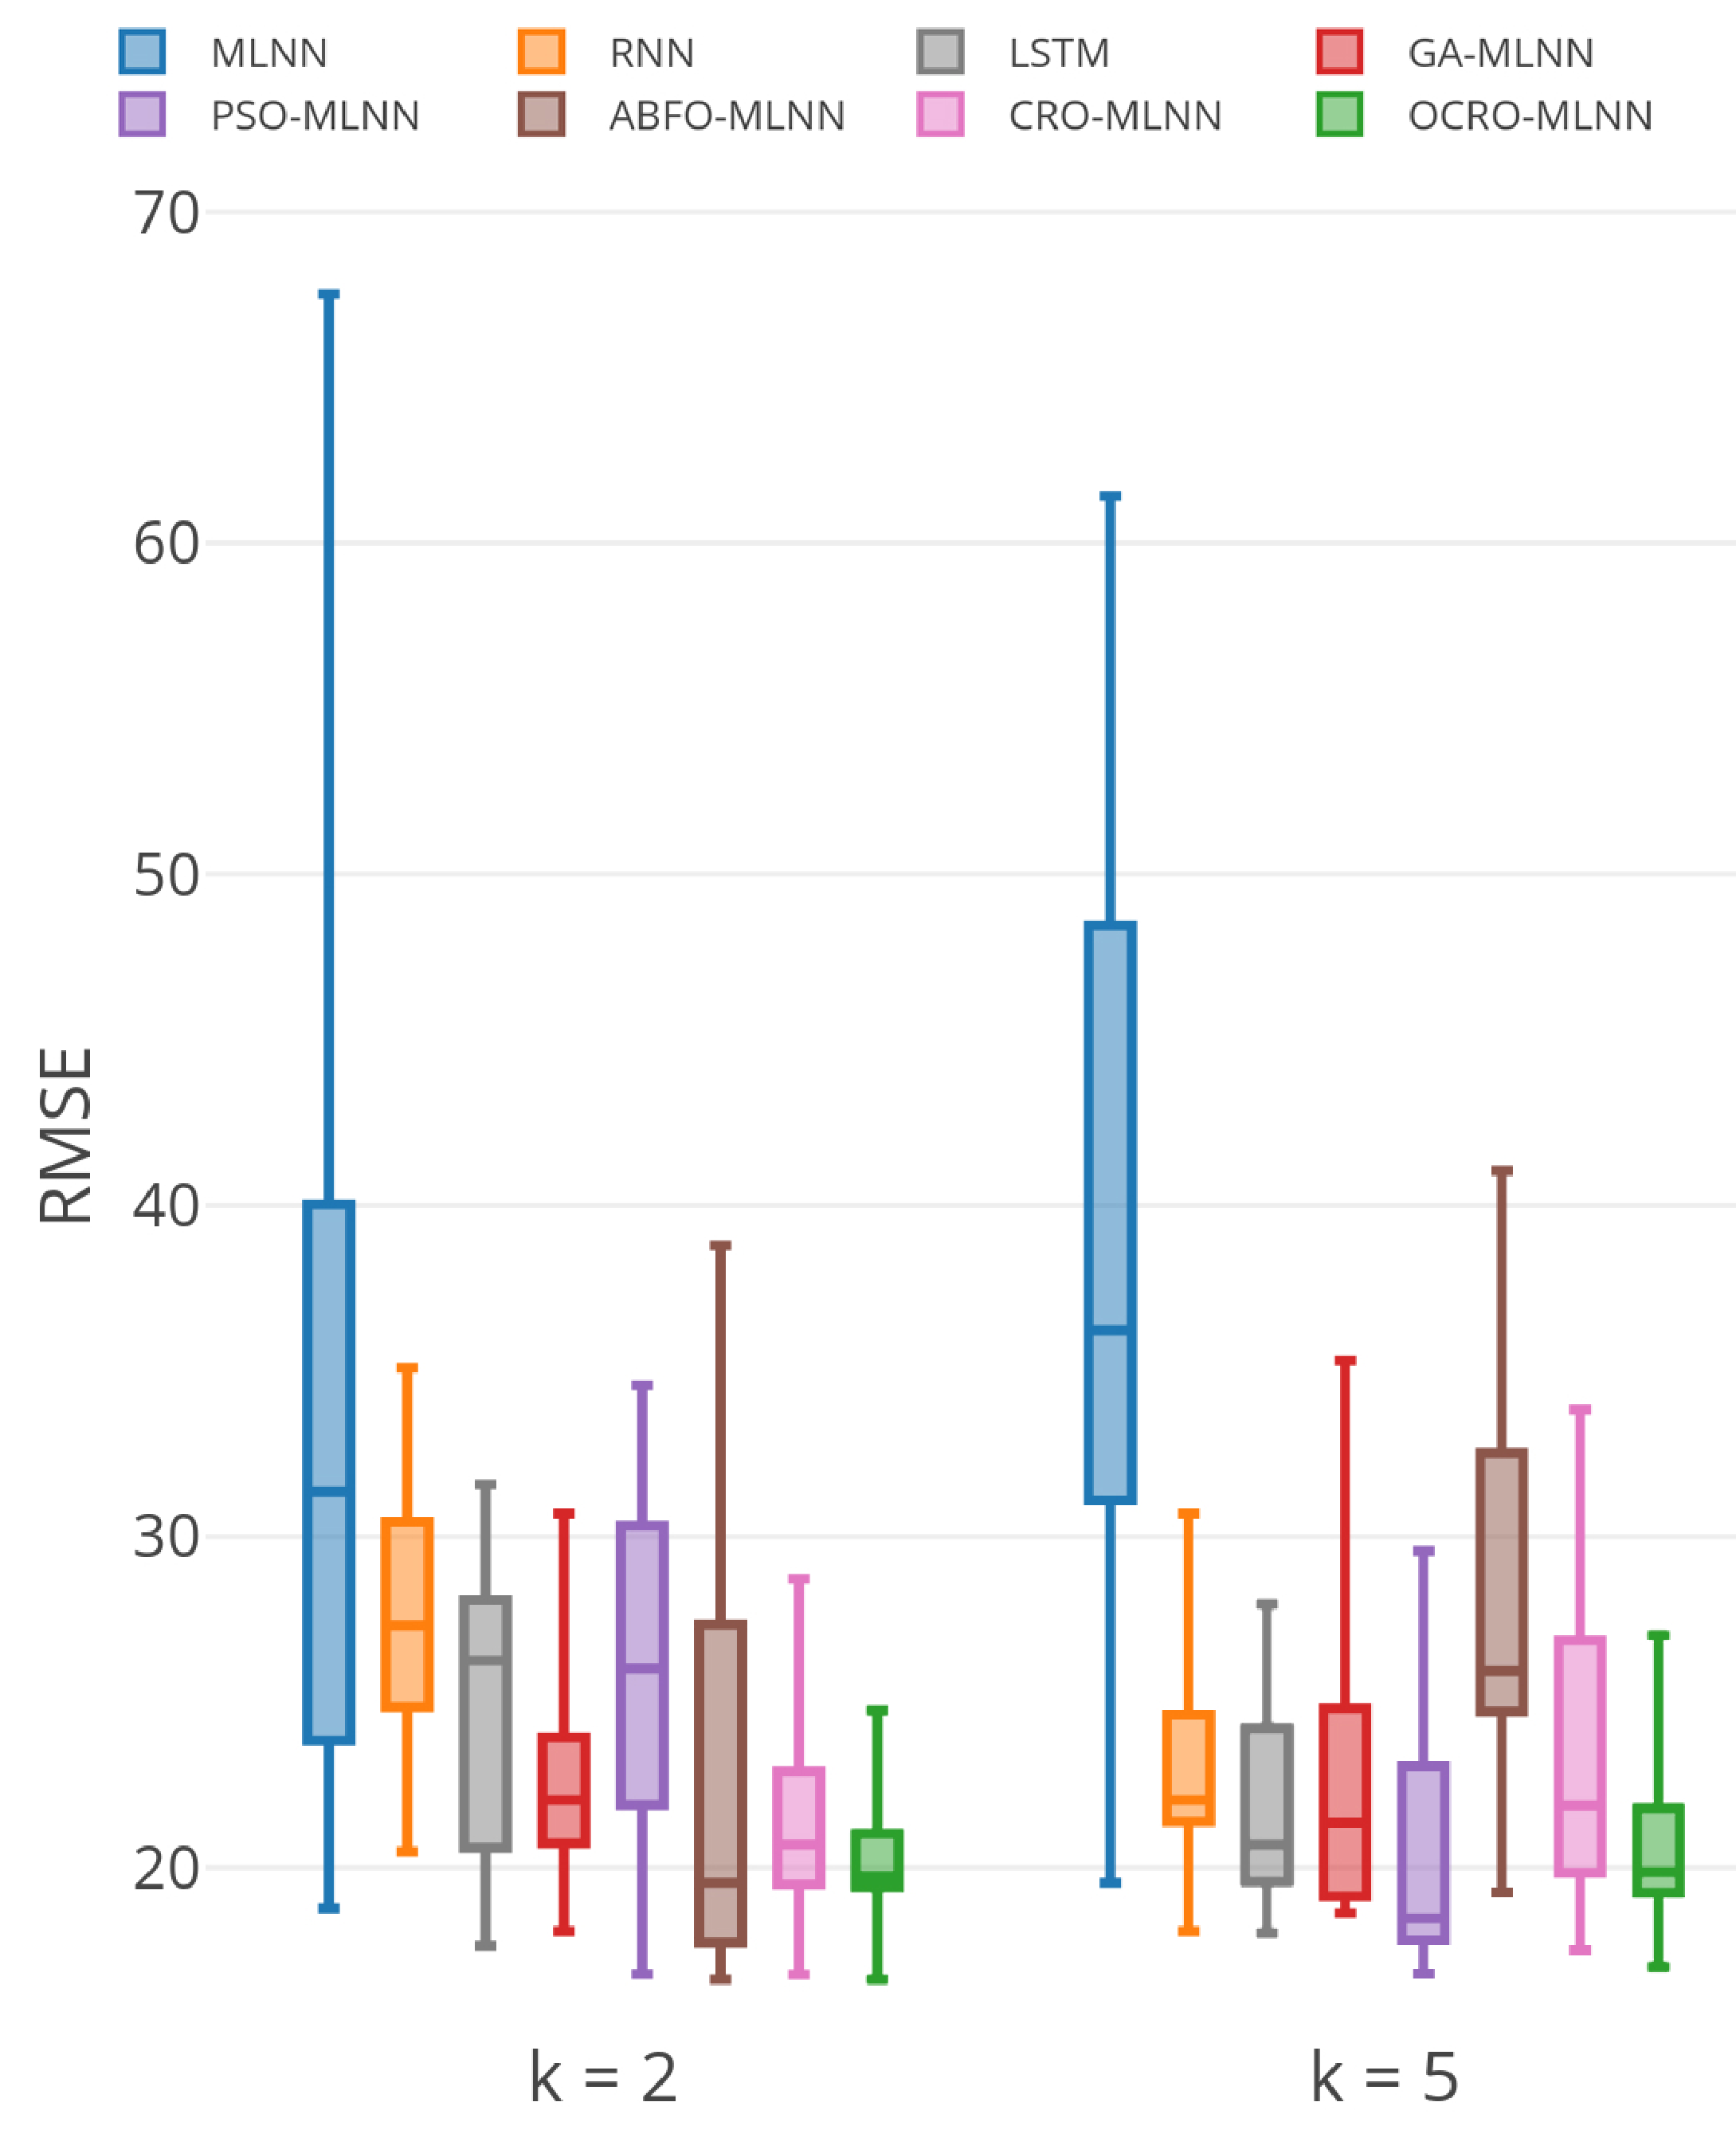
\includegraphics[width=0.45\textwidth =0cm 0cm 0cm 0cm, height = 8cm]{images/pdf/stability/st_wc_2.pdf}
	\end{minipage}
	\caption{RMSE comparison: average of 15 times; univariate data: EU (left), WC (right)} 
	\label{fig:stability_uni}
\end{figure}

\begin{figure}
	\centering
	\begin{minipage}[t]{1\textwidth}
		\centering
		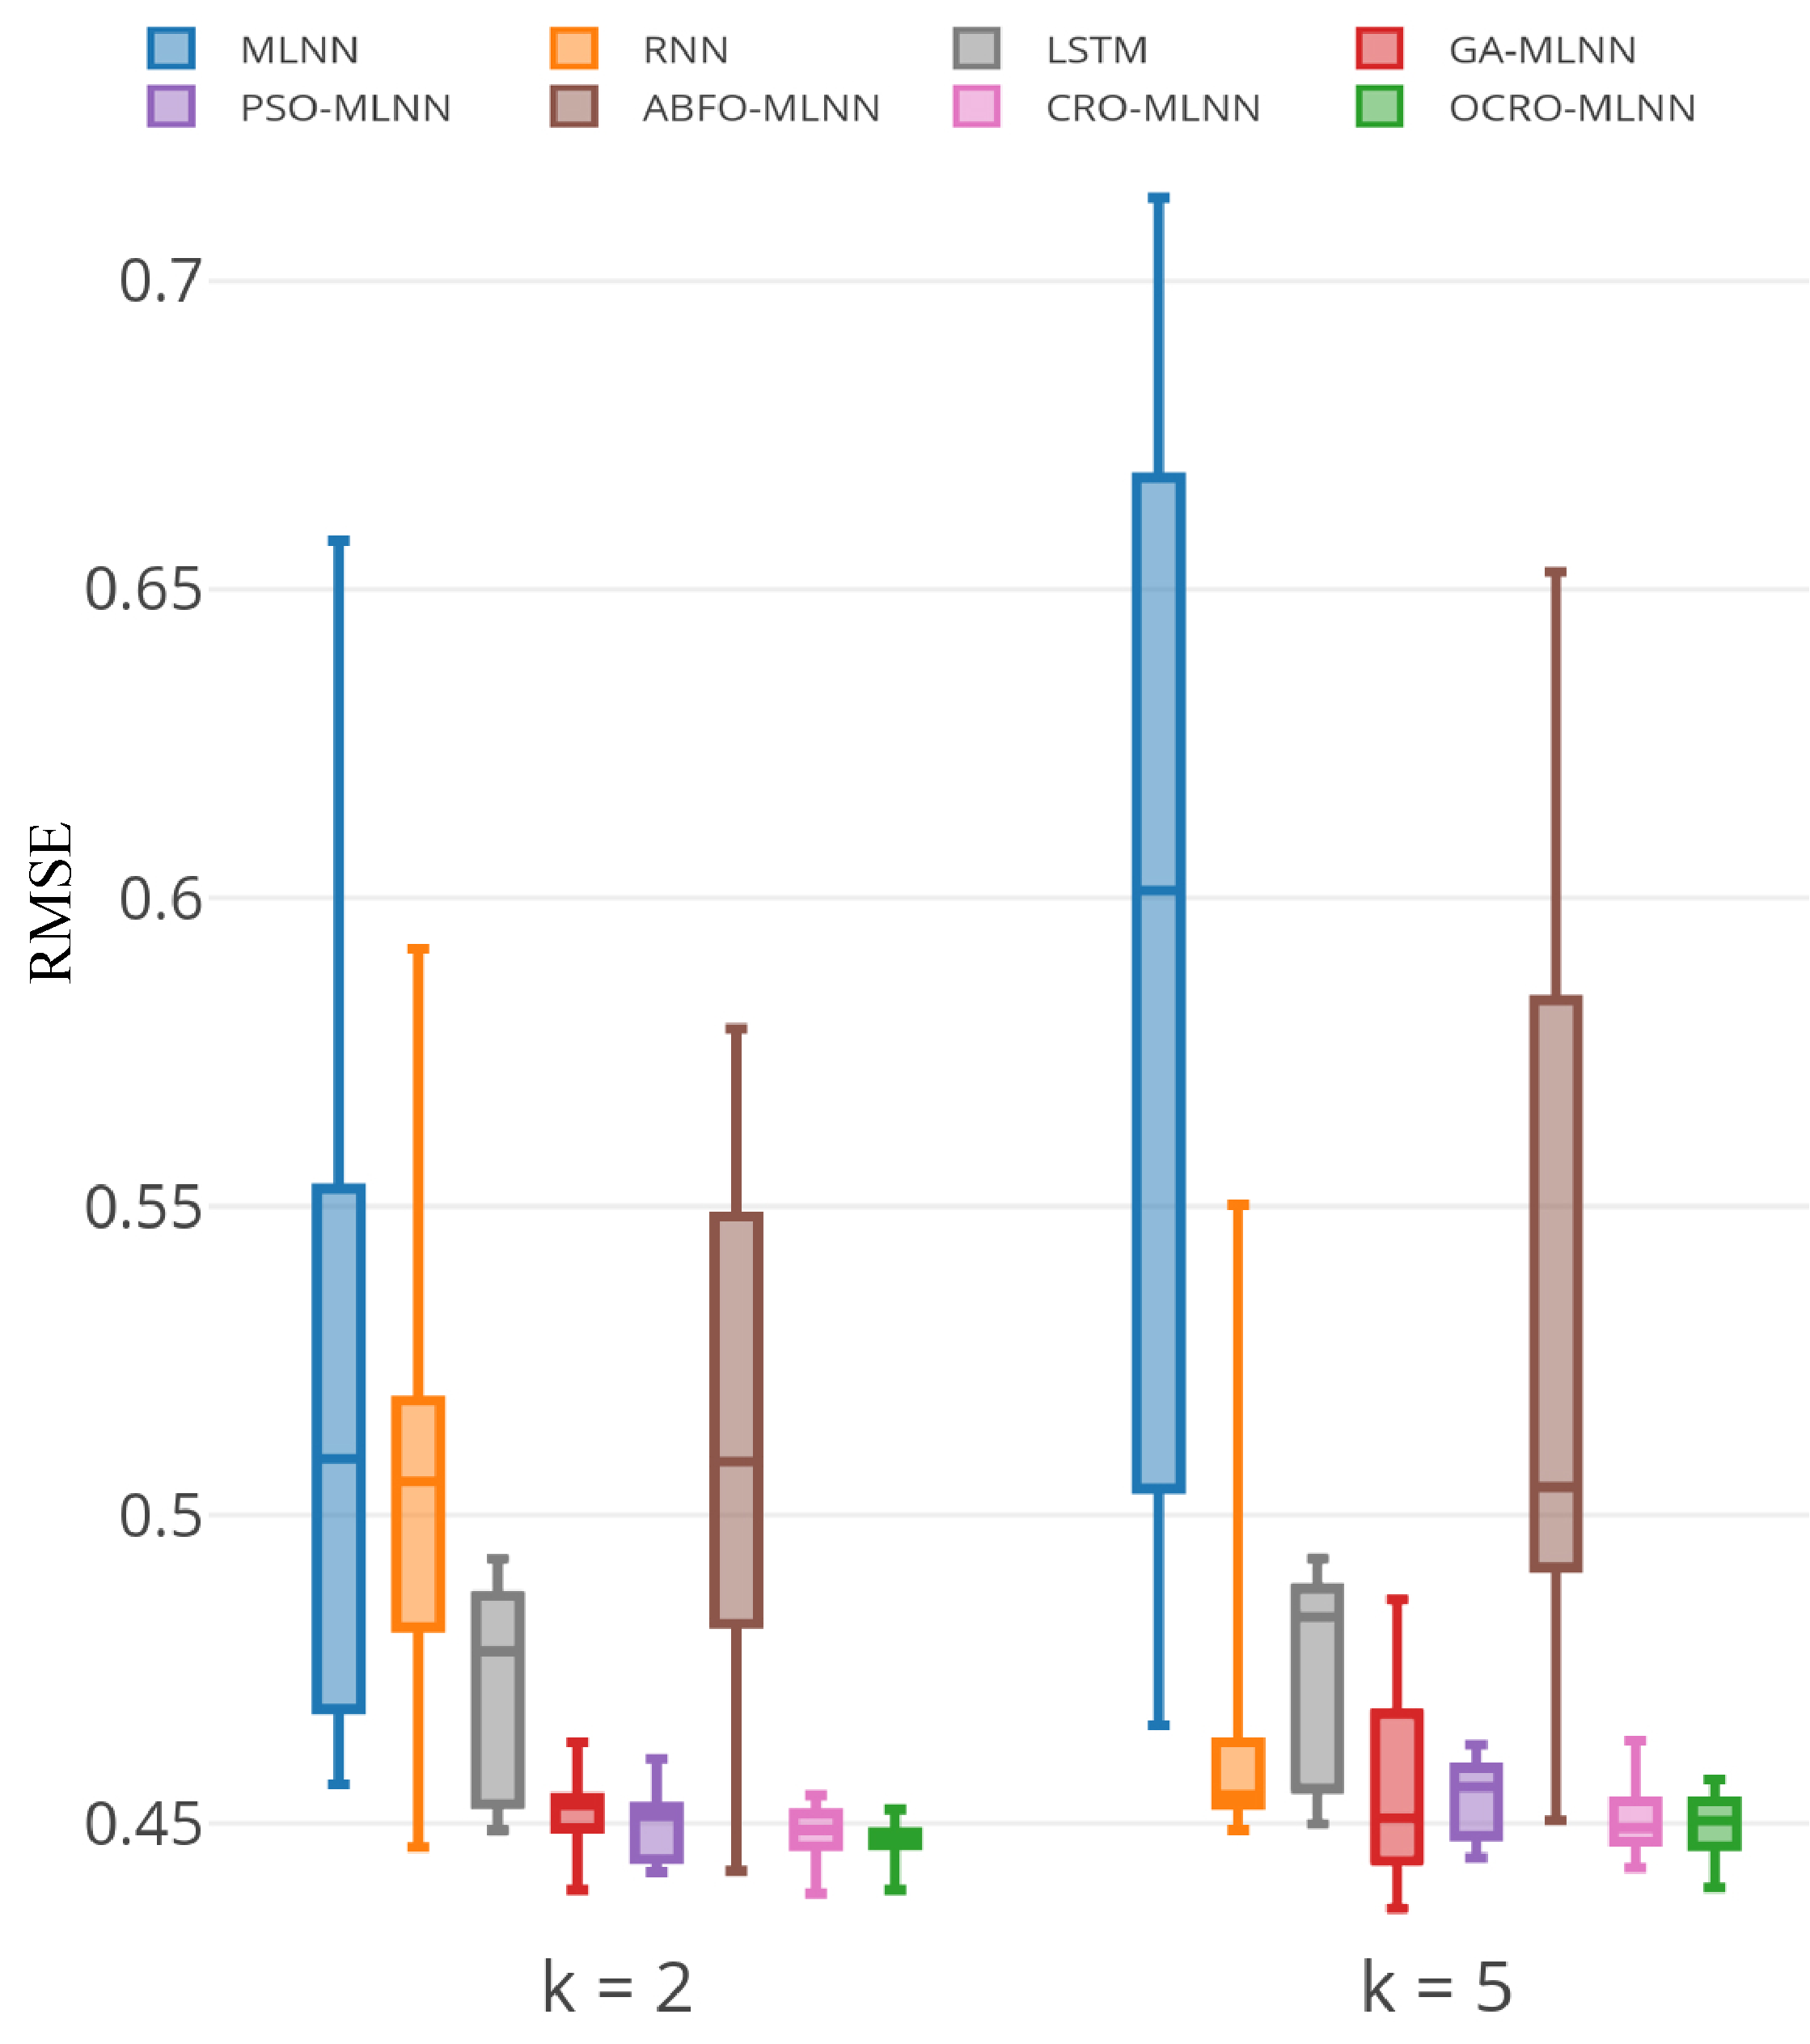
\includegraphics[width=0.45\textwidth =0cm 0cm 0cm 0cm, height = 8cm]{images/pdf/stability/st_cpu_2.pdf}
%	\end{minipage}
%	\begin{minipage}[t]{8cm}
		\centering
		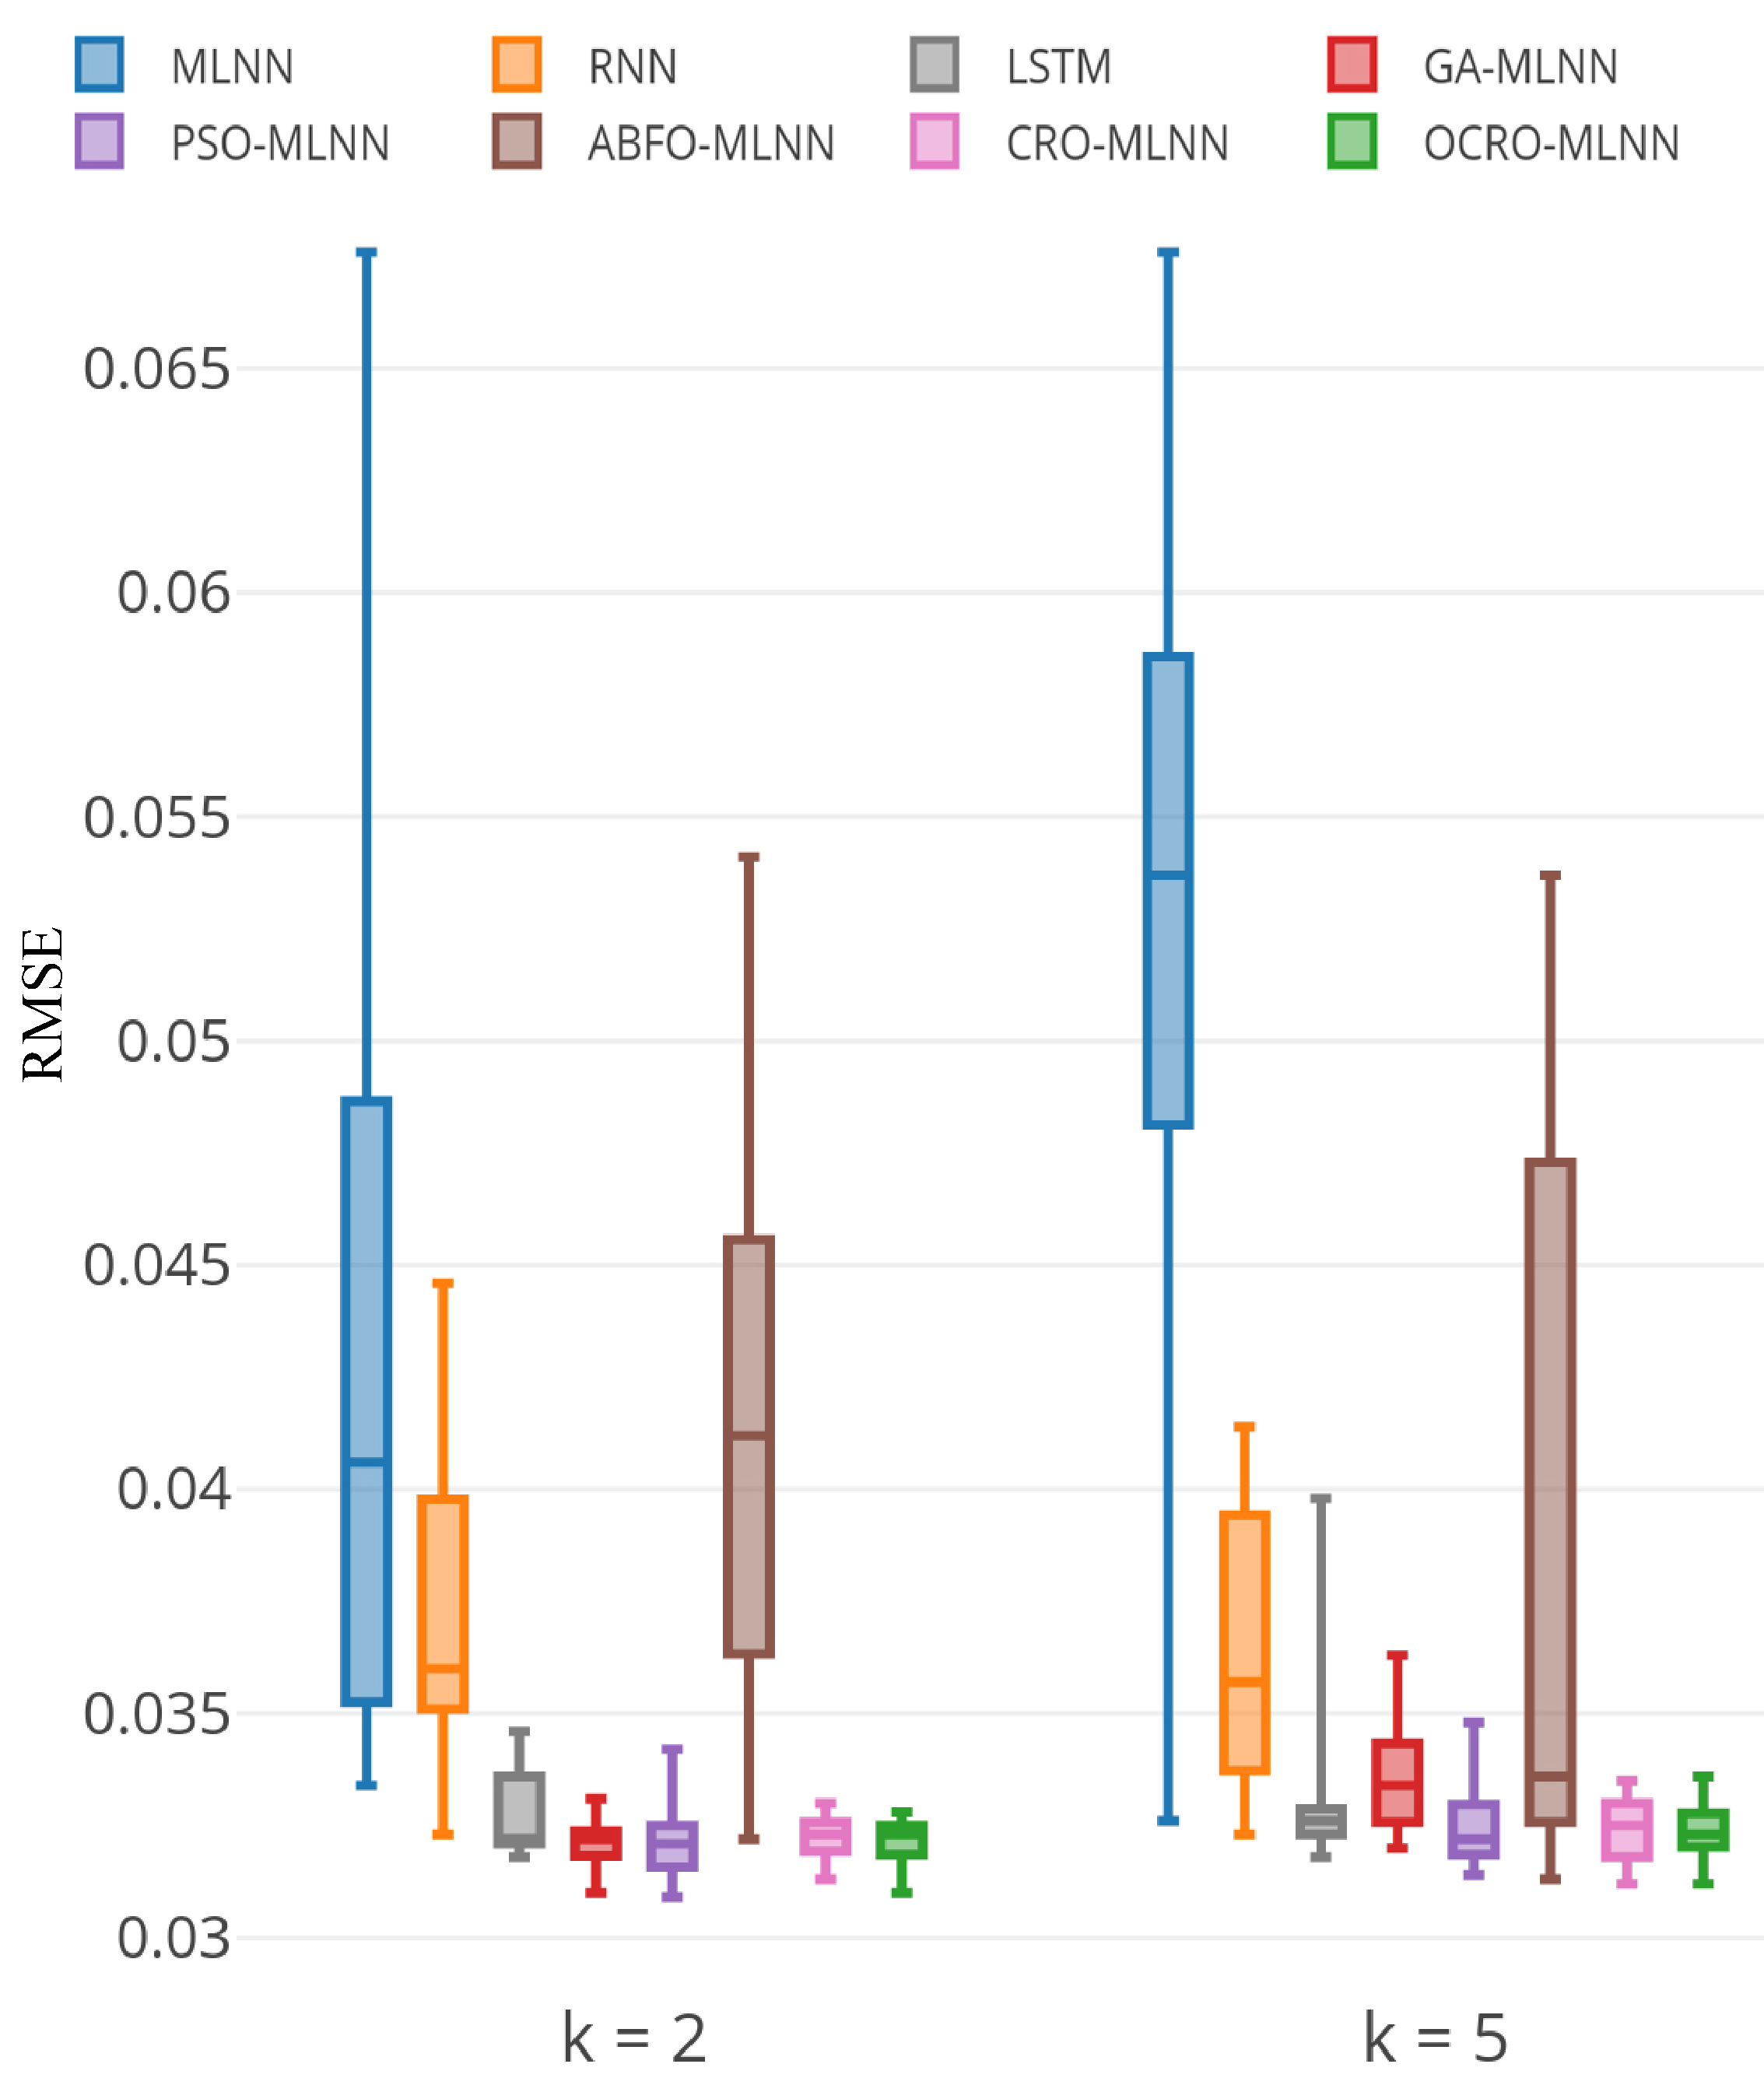
\includegraphics[width=0.45\textwidth =0cm 0cm 0cm 0cm, height = 8.1cm]{images/pdf/stability/st_ram_2.pdf}
	\end{minipage}
	\caption{RMSE comparison: average of 15 times; multivariate data: CPU (left), RAM (right)} 
	\label{fig:stability_multi}
\end{figure}

\subsection{Practical usage of the proposed forecasting approach}
\label{pratical_usage}
In distributed environment, one of the core issues is how to optimize scheduling resources under heavy and changeable computation loads that are made by complex requirements coming from applications. With a set of available resources (e.g. servers, networks, storages), a scheduler must have the capability to make scale in/out decisions to provide computation powers for those applications. Although, the traditional technique for the scaling problem with predefined resource usage thresholds is employed widely in fact, this method has main disadvantage in operation and management of distributed applications: there are always latency between the decision-making moment and its efficiency. This leads to the resources offered to applications does not match with demand in real-time. To deal with the issue, scheduler deployed in distributed systems requires precise estimates resource consumptions. To achieve that capability, the scheduler must have a certain component to predict expected performances of infrastructure systems. The forecast module also is designed in the manner of minimizing costs such as simple prediction model, stability, and runtime constraint, but keeping the good accuracy in order to well operate in practice. 

With the application direction presented above, in this work, through experiments, we proved our proposed OCRO-MLNN model can be applied to schedulers in distributed systems to resolve scaling issue. Moreover, the model also brings the efficiency as desired as compared with other modern learning techniques. Indeed, the tested data was collected from the computing infrastructures (i.e. Google's cluster workload and Internet traffic) and distributed applications (Football world cup's website connection) is used to carry out the model evaluation experiments. 

\section{Conclusion and future works}
\label{conclusion}
This work presented an approach and technique for prediction problem with time series data. The approach is based on idea that build a model with simple structure, stable, low run-time training, but still brings a good accuracy as compare with other modern models. In this way, we created a novel algorithm called Opposition-Based Coral Reefs Optimization (OCRO). Specifically, the proposed algorithm is the combination of Coral Reefs Optimization (CRO) using Opposition-Based Learning (OBL). Thus, we used OCRO together with multi-layer neural network to deal with the forecast problem in the non-linear time series data. By the improvement, our OCRO-MLNN reducing complexity of the model due to faster convergence in comparison with back-propagation technique. 

We are interested in applying the created OCRO-MLNN to distributed systems in order to increase the effectiveness as well as efficiency in allocating resources for applications in the manner of proactiveness. Due to its simplification, fast training, stabilization and forecast performance, the proposed model has the feasibility in applying to the resource schedulers. With the application direction of using in distributed systems, we already tested the proposed OCRO-MLNN with real dataset gathered from those systems, including Google trace cluster data, Internet traffic and popular website's connections. The achieved results through experiments shown that our OCRO-MLNN has advantages in all the proposed criteria listed above as compared with other state-of-the-art models in both univariate and multivariate data. This prove OCRO-MLNN's feasibility in applying to real systems in practice.

The study made contributions in four areas. First, we built OCRO technique by using OBL mechanism for CRO. The improvement helps searching process and avoid local minimum of traditional CRO. Second, a novel forecast model is introduced with the combination of our OCRO technique with MLNN. In which OCRO is used to replace back-propagation. Third, in the terms of evaluation, we conducted comparisons among different prediction models and OCRO-MLNN for time series data. Four, with three real datasets collected from well-known systems, we tested performance of the proposed model as well as other popular methods above. The tests were carried out under three factors, including accuracy, stability, and runtime.

In the future, there are two routes that we plan to do. The first route is to design and develop a resource allocation scheduler which we would like to employ to cloud and high-performance systems. The scheduler thus must process multivariate data with diverse metrics as usual scaling requirement. Besides, a resource allocation decision module also is demanded for the scheduler. The second route is to use and improve several other nature-inspired algorithms, then combine with machine techniques like neural network to serve forecast problem in proactive auto-scalers of distributed systems.

%%%%%
\section*{Acknowledgments} This research is supported by the 
Vietnamese MOETs project No. B2017-BKA-32, Slovak APVV-17-0619 and EU H2020-777533 PROCESS.


%\section*{References}

%%%%%%%%%%%%%%%%%%%%%%%
%% Elsevier bibliography styles
%%%%%%%%%%%%%%%%%%%%%%%
%% To change the style, put a % in front of the second line of the current style and
%% remove the % from the second line of the style you would like to use.
%%%%%%%%%%%%%%%%%%%%%%%

%% Numbered
%\bibliographystyle{model1-num-names}

%% Numbered without titles
%\bibliographystyle{model1a-num-names}

%% Harvard
%\bibliographystyle{model2-names.bst}\biboptions{}

%% Vancouver numbered
%\usepackage{numcompress}\bibliographystyle{model3-num-names}

%% Vancouver name/year
%\usepackage{numcompress}\bibliographystyle{model4-names}\biboptions{authoryear}

%% APA style
%\bibliographystyle{model5-names}\biboptions{authoryear}

%% AMA style
%\usepackage{numcompress}\bibliographystyle{model6-num-names}

%% `Elsevier LaTeX' style
%\bibliographystyle{elsarticle-harv} 
% \bibliographystyle{elsarticle-num}
\bibliographystyle{spmpsci}
\bibliography{references}
%%%%%%%%%%%%%%%%%%%%%%%


\end{document}
\endinput
%%